\documentclass{whureport}
\begin{document}
\thispagestyle{empty}
\tableofcontents
\makeheader
\setcounter{page}{1}
\section{实验内容}
\subsection{实验选题内容}
\subsubsection{Part A 综合装配}
\begin{itemize}
  \item 任务一:在已有实验代码基础上,将1-7章节进行功能综合,形成你自己的一个简易OS。可以实现如下功能:
  \begin{itemize}
  \item 可以考虑使用软盘或者硬盘,启动该OS。
  \item 能够实现你在前面章节所实现的,内存分配与释放。
	\item 能够进行多进程管理,并实现一个有别于本教材上已列出的多进程调度策略,及一个评价该策略性能的小程序。(例如:实现一个多级反馈队列调度算法,并用其尝试调度5-8个任务,输出性能评价信息。)
	\item 所有代码需用目录树结构管理,并添加完整的makefile编译,以及文档
\end{itemize}
	\item 任务二:参照第10章、第11章内容,理清相关代码结构,以及OrangeS所支持的功能,扩展shell,完成如下任务:
\begin{itemize}
  \item 利用当前OrangeS所提供的系统调用和API,编写2个以上可执行程序(功能自定),并编译生成存储在文件系统中
\item 在Shell中调入你所编写的可执行程序,启动并执行进程(注意使用教材中所提供的系统调用来实现)
\item 进程结束后返回Shell
\end{itemize}
\item 任务三:改造任务二的shell,使其能够在同一个shell中,支持多任务执行
\begin{itemize}
  \item 注意现有内存管理可能不支持多程序支持
\item 可执行程序的装入和内存定位问题需要仔细考虑
\end{itemize}
\item 任务四:继续扩展程序,支持基于分页的虚拟内存管理
\begin{itemize}
  \item 重点模拟实现请求调页的功能
  \item 页面替换算法考虑FIFO
\end{itemize}

\end{itemize}

\subsubsection{Part B 安全分析与防御}
\begin{itemize}
  \item 任务一:自我OS安全分析
 \begin{itemize}
  \item 分析提示:可执行文件的篡改、内存破坏漏洞
  \item POC实现:
  \begin{itemize}
  \item 编写一个C程序,该程序查找OS中的可执行文件,对可执行文件添加额外的代码。
  \item 编写一个C程序,该程序查找OS中的可执行文件,对可执行文件添加额外的代码。
\end{itemize}

\end{itemize}
\item 任务二:可信防护之静态度量
\begin{itemize}
  \item 对你的OS进行扩充,编写一个程序模块,该程序模块能够在,当OS加载可执行文件时,对该可执行文件进行完整性校验,并进行比对。
  \item 完整性校验的算法,可采用简单的奇偶校验算法。
  \item 思考:
  \begin{itemize}
  \item 这样的度量,是否能够抵御对可执行文件的篡改?
  \item 完整性校验算法,使用奇偶校验算法,是否存在什么问题?
  \item 完整性校验值应该存在哪里?
\end{itemize}

\end{itemize}
\item 任务三:可信防护之动态度量
\begin{itemize}
  \item 对你的OS进行扩充,编写一个软件中断,该中断能够响应定时中断触发。
  \item 触发时,读取当前运行的进程的内存布局进行,并解析堆栈结构,检查堆栈返回地址是否合法。
  \item 思考:
  \begin{itemize}
  \item 如何理解“合法”的概念?
  \item 你的实现能否抵御POC实现中,第二个攻击?
  \item 这种度量方法的效率如何,存在什么额外的安全问题?
\end{itemize}


\end{itemize}


\end{itemize}


\subsection{小组分工情况}

小组内各个成员都积极参与各个部分的讨论,共同完成这次实验,下面是各个成员主要分工情况:
\begin{itemize}
  \item 彭雨昂参与Part A和Part B全任务
  \item 王浩翔参与Part B全任务
  \item 庞紫萱参与Part A全任务
  \item 唐浩淼参与Part A全任务
\end{itemize}




\section{实验环境}
\begin{itemize}
  \item Ubuntu 16.04.1
  \item VMWare Workstation 16 player
  \item bochs 2.6.8
\end{itemize}



\section{实验方案设计}
\subsection{Part A 任务一}
该任务主要实现一个多级反馈队列调度算法,并且实现评价该策略性能的小程序。考虑到评价和展示该多级反馈队列的信息,我们会打印大量信息,和第十章的一些输出信息重叠在一起会造成影响,于是我们这个任务主要基于第六章r文件夹的代码。

多级反馈队列的\textbf{算法描述}如下:
\begin{itemize}
  \item 进程在进入待调度的队列等待时,首先进入优先级最高的$Q_1$等待。
  \item 首先调度优先级高的队列中的进程。若高优先级中队列中已没有调度的进程,则调度次优先级队列中的进程。例如:$Q_1$、$Q_2$、$Q_3$三个队列,当且仅当在$Q_1$中没有进程等待时才去调度$Q_2$,同理,只有$Q_1$、$Q_2$都为空时才会去调度$Q_3$。
  \item 对于同一个队列中的各个进程,按照FCFS分配时间片调度。比如$Q_1$队列的时间片为N,那么$Q_1$中的作业在经历了N个时间片后若还没有完成,则进入$Q_2$队列等待,若$Q_2$的时间片用完后作业还不能完成,一直进入下一级队列末尾,直至完成。
  \item 在最后一个队列$Q_n$中的各个进程,按照时间片轮转分配时间片调度。
  \item 在低优先级的队列中的进程在运行时,又有新到达的作业,此时须立即把正在运行的进程放回当前队列的队尾,然后把处理机分给高优先级进程。换而言之,任何时刻,只有当第1 到 i-1队列全部为空时,才会去执行第i队列的进程(抢占式)。特别说明,当再度运行到当前队列的该进程时,仅分配上次还未完成的时间片,不再分配该队列对应的完整时间片。
\end{itemize}

基于此,我们的设计思路是:
\begin{itemize}
  \item 在进程表中加入所在队列以及所在队列的位置两个字段,这样就可以表示进程所在队列的位置。
  \item 一个进程不仅需要有一个总时间片了,还应该在进程表中加入在当前队列的剩余时间片。这样当在该队列剩余时间片为0的时候,就会被转移至下一个队列(除了在最后一个队列放在队尾)
  \item 利用\textbf{clocker\_handler()}和\textbf{schedule()}函数配合实现多级反馈调度算法
  \begin{itemize}
  \item 每次时钟中断检查当前进程是否还有总时间片,或者是否在当前队列还有时间片。如果有,那么总时间片和当前队列的时间片都需要减一;
  \item 如果没有,就需要调用\textbf{schedule()}函数处理该进程,把它放入下一个队列(或者当前队列队尾),并且选择下一个进程。
\end{itemize}
\end{itemize}

评价该算法性能的小程序需要打印响应时间、周转时间和等待时间等等信息。比较可惜的是,因为我们基于第六章实现的,在这里操作系统所有进程还是我们手工准备的,而不能进行fork中途加入进程。所以我们多级反馈队列相应也没有实现抢占式算法。这里我们的思路是可以再往进程表中加入提交时间、响应时间、等待时间、周转时间等性能字段。由于是手工准备的进程,那么提交时间都是0时刻;响应时间就是第一次处理该进程的时间,我们可以通过判断进程表的响应字段是否被初始化从而获得响应时间;周转时间是进程结束时刻减去提交时刻,结束时刻只需要在时钟中断中,判断到总时间片是否用完获得结束时刻;等待时间就是周转时间减去进程刚开始初始化的需要运行的时间片。

\subsection{Part A 任务二}
该部分需要拓展shell,为shell添加应用程序。在orange操作系统中,它的实现方式比较简单粗暴。
\begin{itemize}
  \item 应用程序编写
  \begin{itemize}
  \item 将应用程序需要使用的库函数单独链接成一个库文件,然后将写好的应用程序和库文件编译链接起来。
\end{itemize}

  \item 应用程序安装
  \begin{itemize}
  \item 将应用程序打包.tar;
  \item 将tar文件用工具写入磁盘映像的某段特定扇区;
  \item 启动系统时,mkfs()会在文件系统中建立一个新文件cmd.tar,其中inode的i\_start\_sect的值会被设置为上一步写入的扇区的扇区号;
  \item 某个进程会将cmd.tar解包,将其包含的文件存入文件系统。
\end{itemize}

\end{itemize}

\subsection{Part A 任务三}
为实现对多任务执行的支持,需要对 shell 进行改造,使之可以同时解析和执行多条指令。

shell的代码在kernel/main.c中,它由Init()进程fork出来,如下代码所示,Init进程打开了两个shell,分别运行在TTY1和TTY2上。

\begin{lstlisting}[language=c]
void Init()
{
	int fd_stdin  = open("/dev_tty0", O_RDWR);
	assert(fd_stdin  == 0);
	int fd_stdout = open("/dev_tty0", O_RDWR);
	assert(fd_stdout == 1);

	printf("Init() is running ...\n");

	/* extract `cmd.tar' */
	untar("/cmd.tar");
			
	char * tty_list[] = {"/dev_tty1", "/dev_tty2"};

	int i;
	for (i = 0; i < sizeof(tty_list) / sizeof(tty_list[0]); i++) {
		int pid = fork();
		if (pid != 0) { /* parent process */
			printf("[parent is running, child pid:%d]\n", pid);
		}
		else {	/* child process */
			printf("[child is running, pid:%d]\n", getpid());
			close(fd_stdin);
			close(fd_stdout);
			
			shabby_shell(tty_list[i]);
			assert(0);
		}
	}

	while (1) {
		int s;
		int child = wait(&s);
		printf("child (%d) exited with status: %d.\n", child, s);
	}
	assert(0);
}
\end{lstlisting}


shell目前的功能很简单,就是读取命令并且执行之。代码如下所示,shabby\_shell用read()读取用户输入,然后fork()出一个子进程,在子进程中将输入交给execv()来执行。如果用户的输入并不是一个合法的命令,那么shabby\_shel1只是将命令回显出来,不做其他任何处理。

\begin{lstlisting}
void shabby_shell(const char * tty_name)
{
	int fd_stdin  = open(tty_name, O_RDWR);
	assert(fd_stdin  == 0);
	int fd_stdout = open(tty_name, O_RDWR);
	assert(fd_stdout == 1);

	char rdbuf[128];

	while (1) {
		write(1, "$ ", 2);
		int r = read(0, rdbuf, 70);
		rdbuf[r] = 0;

		int argc = 0;
		char * argv[PROC_ORIGIN_STACK];
		char * p = rdbuf;
		char * s;
		int word = 0;
		char ch;
		do {
			ch = *p;
			if (*p != ' ' && *p != 0 && !word) {
				s = p;
				word = 1;
			}
			if ((*p == ' ' || *p == 0) && word) {
				word = 0;
				argv[argc++] = s;
				*p = 0;
			}
			p++;
		} while(ch);
		argv[argc] = 0;

		int fd = open(argv[0], O_RDWR);
		if (fd == -1) {
			if (rdbuf[0]) {
				write(1, "{", 1);
				write(1, rdbuf, r);
				write(1, "}\n", 2);
			}
		}
		else {
			close(fd);
			int pid = fork();
			if (pid != 0) { /* parent */
				int s;
				wait(&s);
			}
			else {	/* child */
				execv(argv[0], argv);
			}
		}
	}

	close(1);
	close(0);
}
\end{lstlisting}

我们利用\&符号分割多条命令,那么我们拓展shabby\_shell能够执行多条命令的思路就是:\begin{itemize}
\item 创建二维字符串数组multi\_argv[MAX\_SHELL\_PROC][MAX\_SHELL\_PROC\_STACK]
  \item 在argv中保存完所有字符串后,我们再对argv进行扫描,把用\&分割的命令分别保存在multi\_argv中
  \item 用for循环进行fork出子进程,同时我们要考虑如下问题
  \begin{itemize}
  \item 父进程利用for循环进行fork,子进程也同样会在该循环
  \item 子进程如果抢占了父进程,那么父进程可能无法fork完所有子进程,导致无法运行多条命令
\end{itemize}

\end{itemize}

上述问题会在实验过程分析中仔细考虑与解决。

\subsubsection{wait和exit}
在shabby\_shell中,还有一个wait函数,wait和exit是一对函数。exit()执行后杀死进程,wait()执行后挂起程序,与fork()相同,这两个函数工作时将会返回EXIT和WAIT消息给MM。在MM中,收到的消息分别由do\_exit()和do\_wait()来处理。

假设进程P有子进程A。而A调用exit(),那么MM将会:
\begin{itemize}
  \item 告诉FS:A退出,请做相应处理。
  \item 释放A占用的内存。
  \item 判断P是否正在WAITING。
  \begin{itemize}
  \item 如果是
  \begin{itemize}
  \item 清除P的WAITING位;
  \item 向P发送消息以解除阻塞(到此P的wait()函数结束);
  \item 释放A的进程表项(到此A的exit()函数结束)。
\end{itemize}

  \item 如果否
  \begin{itemize}
  \item 设置A的HANGING位。
\end{itemize}

\end{itemize}
\item 遍历proc\_table[],如果发现A有子进程B,那么:
\begin{itemize}
  \item 将Init进程设置为B的父进程(换言之,将B过继给Init)。
  \item 判断是否满足Init正在WAITING且B正在HANGING。
  \begin{itemize}
  \item 如果是:
  \begin{itemize}
  \item 清除Init的WAITING位;
  \item 向Init发送消息以解除阻塞(到此Init的wait()函数结束);
  \item 释放B的进程表项(到此B的exit( )函数结束)。
\end{itemize}

  \item 如果否:
  \begin{itemize}
  \item 如果Init正在WAITING但B并没有HANGING,那么“握手”会在将来B调用exit()时发生;
  \item 如果B正在HANGING但Init并没有WAITING,那么“握手”会在将来Init调用wait()时发生。
\end{itemize}

\end{itemize}

\end{itemize}

\end{itemize}

如果P调用wait(),那么MM将会:

\begin{itemize}
  \item 遍历proc\_tabel[],如果发现A是P的子进程,并且它正在HANGING,那么:
  \begin{itemize}
  \item 向P发送消息以解除阻塞(到此P的wait()函数结束);
  \item 释放A的进程表项(到此A的exit()函数结束)。
\end{itemize}

  \item 遍历proc\_tabel[],如果发现A是P的子进程,并且它正在HANGING,那么:
  \begin{itemize}
  \item 设P的WAITING位。
\end{itemize}

  \item 如果P压根儿没有子进程,则:
  \begin{itemize}
  \item 向P发送消息,消息携带一个表示出错的返回值(到此P的wait()函数结束)。
\end{itemize}

\end{itemize}


\subsection{Part A 任务四}
这一个任务属实是炼狱难度了。首先分析当前oranges中的内存管理算法,在满足进阶功能的同时,设计实现基于分页的虚拟内存管理算法。oranges在之前的章节中实现过一个非常简单的分页,但是我们仔细看第十章的代码,发现他并没有使用分页进行管理。

\subsubsection{IPC}
在回顾oranges的内存管理机制前,先简单介绍一下它的IPC机制,IPC机制在后面都非常重要。oranges os采用的是微内核,不再像Linux那样有许许多多的系统调用,在这里系统调用的种类总共有三个,那就SEND、RECEIVE和BOTH。首先看看Minix是如何用这三种系统调用实现fork()函数的。

\begin{figure}[H]
\centering
%[width=0.8\textwidth]
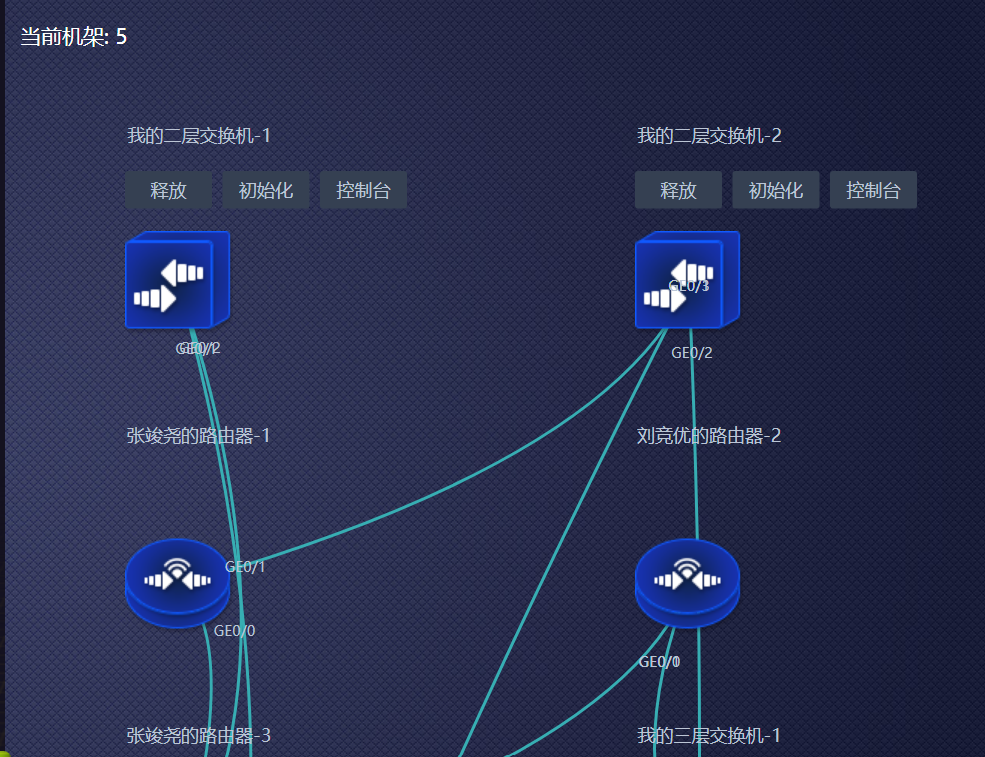
\includegraphics[width=0.55\textwidth]{1}
\end{figure}


用户进程对fork()的调用将最终转化成调用内核态的函数sys\_call(),消息(即图中的m)的地址这时已经作为参数被传递进来, sys\_call()可以据此得知m的内容,并在适当的时候将内容传递给MM,MM的工作其实说起来很简单,它不断地获取并处理消息,所以它能够得到用户进程发送的m,并将其存放在mm\_in中。当MM通过获得的mm\_in得知了消息的内容是要进行fork操作,它就进一步调用其do\_fork()完成整个过程。

因此首先oranges os添加了一个系统调用sendrec。sys\_sendrec 这个函数被设计得相当简单,它可以描述为:把SEND消息交给msg\_send()处理,把RECEIVE消息交给msg\_receive()处理。

并且进程表中添加了如下新的字段,所有增加的这些成员都是跟消息机制有关的:
\begin{itemize}
  \item \textbf{p\_flags}用于标明进程的状态。目前它的取值可以有三种(后续有了fork后会增加几种):
  \begin{itemize}
  \item \textbf{0:}进程正在运行或准备运行。
  \item \textbf{SENDING:}进程处于发送消息的状态。由于消息还未送达,进程被阻塞。
  \item \textbf{RECEIVING:}进程处于接收消息的状态。由于消息还未收到,进程被阻塞。
\end{itemize}
\item \textbf{p\_msg}指向消息体的指针。
\item ...
\end{itemize}

假设有进程A想要向B发送消息M,那么过程将会是这样的:
\begin{enumerate}
	\item A首先准备好M。
	\item  A通过系统调用sendrec,最终调用msg\_send。
	\item 简单判断是否发生死锁。
	\item 判断目标进程B是否正在等待来自A的消息:
	\begin{itemize}
  \item 如果是:消息被复制给B, B被解除阻塞,继续运行;
  \item 如果否:A被阻塞,并被加入到B的发送队列中。
\end{itemize}

\end{enumerate}

假设有进程B想要接收消息(来自特定进程、中断或者任意进程),那么过程将会是这样的:

\begin{enumerate}
	\item B准备一个空的消息结构体M,用于接收消息。
	\item B通过系统调用sendrec,最终调用msg\_receive。
	\item 判断B是否有个来自硬件的消息(通过has\_int\_msg),如果是,并且B准备接收来自中断的消息或准备接收任意消息,则马上准备一个消息给B,并返回。
	\item 如果B想接收来自任意进程的消息,则从自己的发送队列中选取第一个(如果队列非空的话),将其消息复制给M。
	\item 如果B是想接收来自特定进程A的消息,则先判断A是否正在等待向B发送消息,若是的话,将其消息复制给M。
	\item 如果此时没有任何进程发消息给B,B会被阻塞。
\end{enumerate}



\subsubsection{内存管理机制}
在前面几章的实验中,我们知道,分段机制通过GDT与LDT实现,每个进程有一个LDT描述符中包含了段基址,段限长等与分段有关的信息。如下图所示展示了进程,进程表与GDT,LDT的关系:

\begin{figure}[H]
\centering
%[width=0.8\textwidth]
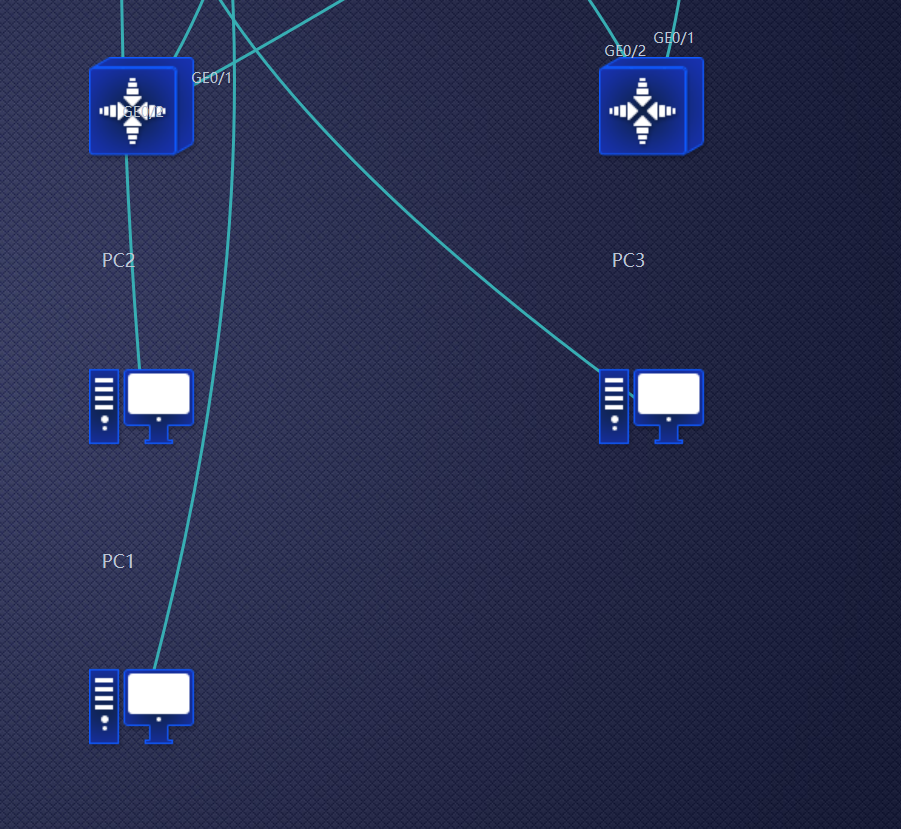
\includegraphics[width=0.8\textwidth]{2}
\end{figure}


随后我们通过fork()函数来了解oranges os的内存管理机制。fork()源码如下:
\begin{lstlisting}
PUBLIC int fork()
{
	MESSAGE msg;
	msg.type = FORK;

	send_recv(BOTH, TASK_MM, &msg);
	assert(msg.type == SYSCALL_RET);
	assert(msg.RETVAL == 0);

	return msg.PID;
}
\end{lstlisting}

他通过消息传递机制,发送和接收TASK\_MM的消息,并且返回PID。task\_mm函数源码如下,它接收到消息的类型为FORK,然后调用do\_fork()函数。

\begin{lstlisting}
PUBLIC void task_mm()
{
	init_mm();

	while (1) {
		send_recv(RECEIVE, ANY, &mm_msg);
		int src = mm_msg.source;
		int reply = 1;

		int msgtype = mm_msg.type;

		switch (msgtype) {
		case FORK:
			mm_msg.RETVAL = do_fork();
			break;
		case EXIT:
			do_exit(mm_msg.STATUS);
			reply = 0;
			break;
		/* case EXEC: */
		/* 	mm_msg.RETVAL = do_exec(); */
		/* 	break; */
		case WAIT:
			do_wait();
			reply = 0;
			break;
		default:
			dump_msg("MM::unknown msg", &mm_msg);
			assert(0);
			break;
		}

		if (reply) {
			mm_msg.type = SYSCALL_RET;
			send_recv(SEND, src, &mm_msg);
		}
	}
}
\end{lstlisting}


do\_fork()函数内容有些多,其具体分为五部分:
\begin{itemize}
  \item 第一部分是分配进程表,从数组proc\_table[]中寻找一个空项,用于存放子进程的进程表。接下来将父进程的进程表原原本本地赋给子进程。
  \item 第二部分是分配内存。由于子进程是父进程的副本,所以首先需要得到父进程的内存占用情况,这由读取LDT来完成。
  \item 有了父进程的内存占用情况,就用分配内存的函数为alloc\_mem()分配内存。
  \item ...
\end{itemize}


我们仔细去看一下alloc\_mem()函数。其中最关键的就是第22行,oranges os简单地只给每个进程一个PROC\_IMAGE\_SIZE\_DEFAULT大小的内存,然后根据pid的值按顺序从PROCS\_BASE处向上分配内存。

\begin{lstlisting}
/*****************************************************************************
 *                                alloc_mem
 *****************************************************************************/
/**
 * Allocate a memory block for a proc.
 * 
 * @param pid  Which proc the memory is for.
 * @param memsize  How many bytes is needed.
 * 
 * @return  The base of the memory just allocated.
 *****************************************************************************/
PUBLIC int alloc_mem(int pid, int memsize)
{
	assert(pid >= (NR_TASKS + NR_NATIVE_PROCS));
	if (memsize > PROC_IMAGE_SIZE_DEFAULT) {
		panic("unsupported memory request: %d. "
		      "(should be less than %d)",
		      memsize,
		      PROC_IMAGE_SIZE_DEFAULT);
	}

	int base = PROCS_BASE +
		(pid - (NR_TASKS + NR_NATIVE_PROCS)) * PROC_IMAGE_SIZE_DEFAULT;

	if (base + memsize >= memory_size)
		panic("memory allocation failed. pid:%d", pid);

	return base;
}
\end{lstlisting}

fork()后我们还需要通过exec()运行新的进程,和fork一样也是通过消息传递机制实现,我们直接来看do\_exec的源码。最主要的是在30-44行代码,这里把新的elf文件覆盖原来的内存,其中va2la函数就是把虚拟地址转化为线性地址,其实由于没有开启虚拟内存,这里的线性地址等于物理地址。

\begin{lstlisting}
PUBLIC int do_exec()
{
	/* get parameters from the message */
	int name_len = mm_msg.NAME_LEN;	/* length of filename */
	int src = mm_msg.source;	/* caller proc nr. */
	assert(name_len < MAX_PATH);

	char pathname[MAX_PATH];
	phys_copy((void*)va2la(TASK_MM, pathname),
		  (void*)va2la(src, mm_msg.PATHNAME),
		  name_len);
	pathname[name_len] = 0;	/* terminate the string */

	/* get the file size */
	struct stat s;
	int ret = stat(pathname, &s);
	if (ret != 0) {
		printl("{MM} MM::do_exec()::stat() returns error. %s", pathname);
		return -1;
	}

	/* read the file */
	int fd = open(pathname, O_RDWR);
	if (fd == -1)
		return -1;
	assert(s.st_size < MMBUF_SIZE);
	read(fd, mmbuf, s.st_size);
	close(fd);

	/* overwrite the current proc image with the new one */
	Elf32_Ehdr* elf_hdr = (Elf32_Ehdr*)(mmbuf);
	int i;
	for (i = 0; i < elf_hdr->e_phnum; i++) {
		Elf32_Phdr* prog_hdr = (Elf32_Phdr*)(mmbuf + elf_hdr->e_phoff +
			 			(i * elf_hdr->e_phentsize));
		if (prog_hdr->p_type == PT_LOAD) {
			assert(prog_hdr->p_vaddr + prog_hdr->p_memsz <
				PROC_IMAGE_SIZE_DEFAULT);
			phys_copy((void*)va2la(src, (void*)prog_hdr->p_vaddr),
				  (void*)va2la(TASK_MM,
						 mmbuf + prog_hdr->p_offset),
				  prog_hdr->p_filesz);
		}
	}

	/* setup the arg stack */
	int orig_stack_len = mm_msg.BUF_LEN;
	char stackcopy[PROC_ORIGIN_STACK];
	phys_copy((void*)va2la(TASK_MM, stackcopy),
		  (void*)va2la(src, mm_msg.BUF),
		  orig_stack_len);

	u8 * orig_stack = (u8*)(PROC_IMAGE_SIZE_DEFAULT - PROC_ORIGIN_STACK);

	int delta = (int)orig_stack - (int)mm_msg.BUF;

	int argc = 0;
	if (orig_stack_len) {	/* has args */
		char **q = (char**)stackcopy;
		for (; *q != 0; q++,argc++)
			*q += delta;
	}

	phys_copy((void*)va2la(src, orig_stack),
		  (void*)va2la(TASK_MM, stackcopy),
		  orig_stack_len);

	proc_table[src].regs.ecx = argc; /* argc */
	proc_table[src].regs.eax = (u32)orig_stack; /* argv */

	/* setup eip & esp */
	proc_table[src].regs.eip = elf_hdr->e_entry; /* @see _start.asm */
	proc_table[src].regs.esp = PROC_IMAGE_SIZE_DEFAULT - PROC_ORIGIN_STACK;

	strcpy(proc_table[src].name, pathname);

	return 0;
}
\end{lstlisting}


\subsubsection{分页实现思路}
关于分页机制的细节我们不在这里过多赘述,在x86中,cpu支持硬件实现的两级页表,通过cr3寄存器存储的页目录基址寻址到页目录,接下来从页目录中查找到相应页表对应的地址,接下来从页表中查找对应的页表项pte,最后再寻址到物理内存。

我们可以发现,orange’s虽然启用了操作系统的分页机制并且初始化了页表和页目录,但并没有利用这个分页机制进行内存管理,在kernel的代码中,我们可以发现,操作系统在引导过程中在0x100000即64KB位置建立了连续的页表和页目录,并且将系统的全部内存范围都做了线性映射,在之后操作系统的整个生命周期中,这个页表都是固定的,不会再发生变化,cr3的值也不会发生变化。


参照linux中对于内存管理的实现,在linux中,每个进程都会有自己的页表,通过页表而不是分段机制管理自己的可用内存,因此要把分页机制充分利用,我们不止需要一个固定的页表,因此我们需要为每个进程创建自己的页表,并且利用页表来进行进一步的内存映射,例如消除内存空洞等,我们可以为每个进程创建独立的地址映射,并把地址映射保存在进程的页表中,在进程上下文切换时切换页表,这样就可以充分利用操作系统的分页机制,进一步完善内存管理机制。因此我们实现的分页的整体思路为:

\begin{itemize}
  \item 进程表的stackframe中要添加页目录基址pde
  \item 在exec中装入elf文件的时候,添加一层线性地址到物理地址的映射。
  \item 还需要在exec后面放入页表,该页表和上面的映射相关。
\end{itemize}


\subsection{Part B 任务一}
该任务要编写一个 C 程序,该程序查找 OS 中的可执行文件,对可执行文件添加额外代码;还需要编写一个程序,可对存在内存破坏漏洞的代码进行缓冲区溢出,控制返回地址到指定位置。

\subsubsection{ELF文件注入}


shellcode 是一段能够被执行的机器码,其注入方式主要有代码空洞和新增节两种,下面简单介绍两种方式的注入流程:

\paragraph{代码空洞注入}
\begin{itemize}
  \item 以可读写方式打开文件;
  \item 找一个大小合适的 code cave;
  \item 将 shellcode 嵌入到 code cave 中;
  \item 修改 entrypoint 指向 shellcode 的开头
\end{itemize}

\paragraph{新增节注入}
我们首先介绍ELF文件格式:

\begin{figure}[H]
\centering
%[width=0.8\textwidth]
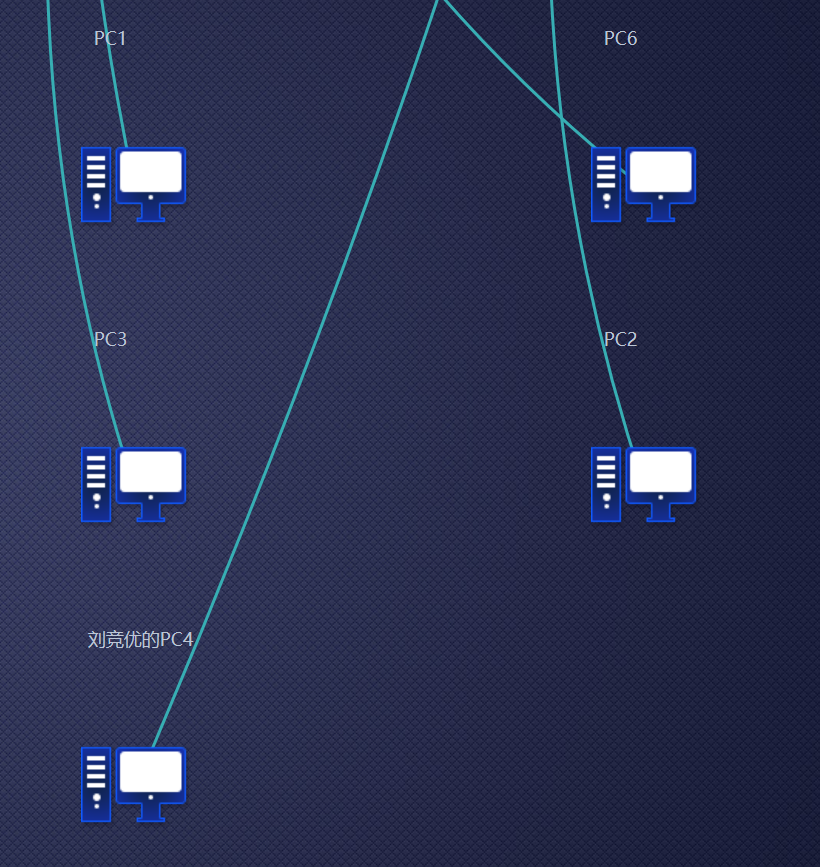
\includegraphics[width=0.6\textwidth]{3}
\end{figure}

文件开始处是一个 ELF 头部(ELF Header),用来描述整个文件的组织。节区部 分包含链接视图的大量信息:指令、数据、符号表、重定位信息等等。

程序头部表(Program Header Table),如果存在的话,告诉系统如何创建进程映像。 用来构造进程映像的目标文件必须具有程序头部表,可重定位文件不需要这个表。

节区头部表(Section Heade Table)包含了描述文件节区的信息,每个节区在表中 都有一项,每一项给出诸如节区名称、节区大小这类信息。用于链接的目标文件必须包 含节区头部表,其他目标文件可以有,也可以没有这个表。

\textit{注意: 尽管图中显示的各个组成部分是有顺序的,实际上除了 ELF 头部表以外, 其他节区和段都没有规定的顺序}


于是,我们ELF文件新增节注入思路如下:
\begin{itemize}
  \item 存储相关原始数据,如原文件入口地址
  \item 修正 ELF 头部 中的 e\_shoff ,增加 PAGESIZE 大小(操作系统页式系统,一页默认4k)
  \item 修正 第一个程序头部表,第一个头部特殊对待,因为要插入自己注入的程序,所以要把第一个头部扩容,把p\_filesz 和 p\_memsz 增加 PAGESIZE 大小或者 注入程序的大小
  \item 修正 ELF 头部 中的 e\_entry ,指向 p\_vaddr + p\_filesz
  \item 修正程序头部表偏移地址p\_offset ,增加 PAGESIZE 大小
  \item 修正节区 sh\_offset ,增加 PAGESIZE 大小
  \item 修正注入程序机器码,如:修正数据段存储地址(从新的elfh.e\_entry开始计算程序首地址),最后要加上跳转指令,即跳转到原来的e\_entry(刚开始记录的)
  \item 首先存储原来目标节区头到末尾的数据,然后插入修正后的注入程序的机器码,之后通过插入0的方式让插入区块扩充到 PAGESIZE (4k)
  \item 再把存储的数据接在后面插入
\end{itemize}

\subsubsection{缓冲区溢出与ROP}

栈溢出指的是程序向栈中某个变量中写入的字节数超过了这个变量本身所申请的字节数,因而导致与其相邻的栈中的变量的值被改变。这种问题是一种特定的缓冲区溢出漏洞,类似的还有堆溢出,bss 段溢出等溢出方式。栈溢出漏洞轻则可以使程序崩溃,重则可以使攻击者控制程序执行流程。此外,我们也不难发现,发生栈溢出的基本前提是

\begin{itemize}
  \item 程序必须向栈上写入数据。
  \item 写入的数据大小没有被良好地控制。
\end{itemize}


在内存中,数据的存放位置如下:

\begin{figure}[H]
\centering
%[width=0.8\textwidth]
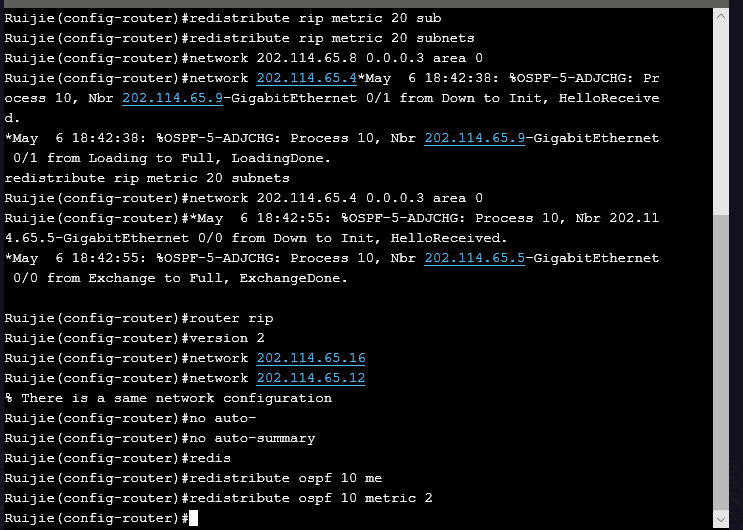
\includegraphics[width=0.4\textwidth]{4}
\end{figure}

在计算机向缓冲区内填充数据位数时,如果超过了缓冲区本身的容量,溢出 的数据会覆盖在合法数据上。那么尝试输入特定数据并覆盖合法数据,执行设计 好的程序功能。假设我们定义了一个数组 buff,借其进行缓冲区溢出攻击,那 么在攻击完成后,最终 buff 地址会覆盖 main 函数的返回地址,成功覆盖返回地 址后,main 函数结束就会跳转到 buff,执行我们的 shellcode。

\begin{figure}[H]
\centering
%[width=0.8\textwidth]
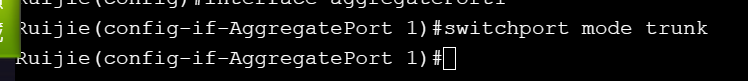
\includegraphics[width=0.6\textwidth]{5}
\end{figure}


\subsection{Part B 任务二}
对你的OS进行扩充,编写一个程序模块,该程序模块能够在,当OS加载可执行文件时,对该可执行文件进行完整性校验,并进行比对。

因此我们思路如下:
\begin{itemize}
  \item 在untar把应用程序装载到os时,计算一个校验码
  \item 在exec运行时,也计算一遍校验码并且和之前的校验码进行比较
\end{itemize}

如果采用简单的奇偶校验,就不能有效防止对可执行文件的篡改。因为攻击者篡改完可执行文件后,可以计算当前校验码和原始校验码的差别,然后通过修改elf文件中一些代码空洞,使得校验码和原始校验码相等。因此我们的校验码计算借助了AES加密(在Part A 任务二中实现了AES,当时没看到Part B 任务二,不然肯定会实现MD5),加大了攻击者篡改难度。我们把untar时候的校验码直接保存在内核内存中,因此攻击者其实可以看到校验码,但由于我们利用了更复杂的校验码计算方法,即使看到校验码,也无法轻易去攻击。

\subsection{Part B 任务三}

迄今为止 ,发生次数最多、最常见的安全漏洞仍是基于栈的缓冲区溢出, 对于这种类型漏洞的最常见利用方式是:在栈中精心构造二进制串溢出原有数据结构进而改写函数返回地址,使其跳转到位于栈中的Shellcode 执行。如果使栈上数据不可执行,那么就可以阻止这种漏洞利用方式的成功实施。 而DEP就是通过使可写内存不可执行或使可执行内存不可写来消除类似的威胁。

DEP - 数据执行保护的缩写,Data Execution Prevention。他是一套软硬件技术,能够在内存上执行额外检查以帮助防止在系统上运行恶意代码。其基本原理是将数据所在内存页标识为不可执行,当程序溢出成功转入shellcode时,程序会尝试在数据页面上执行指令,此时CPU就会抛出异常,而不是去执行恶意指令。

\begin{figure}[H]
	\centering
	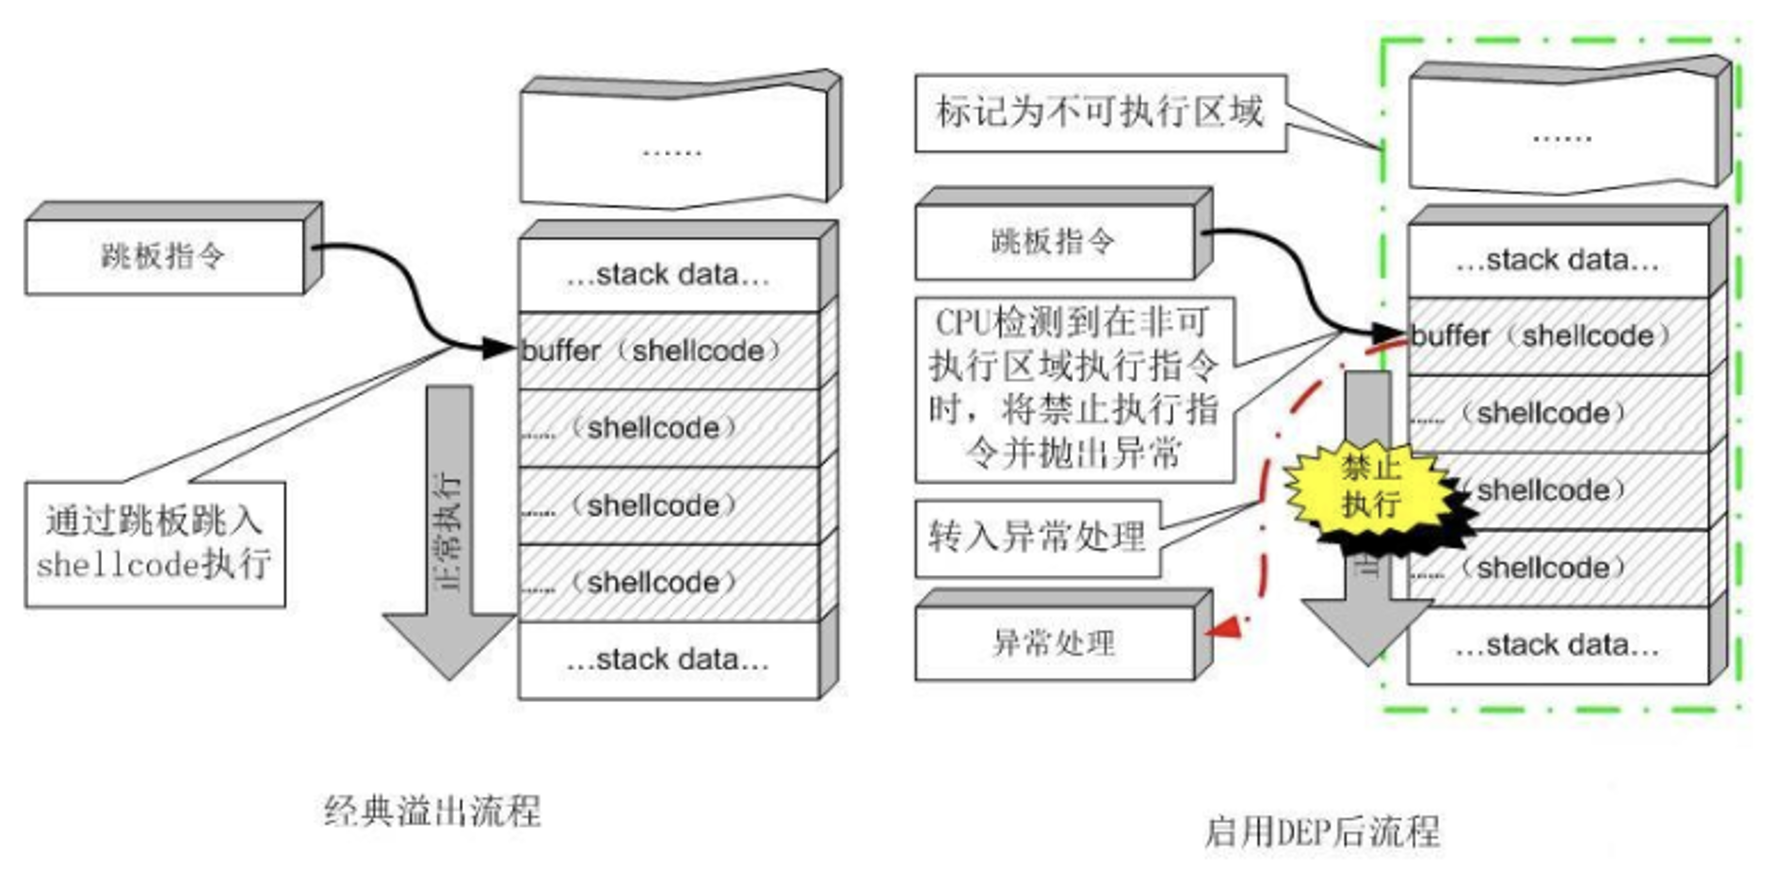
\includegraphics[width=0.8\textwidth]{whx17}
\end{figure}


在这次实验中,我们模拟这种思路,对这一模式进行了简化,我们对程序运行时的情况进行判断,判断是否在栈区运行,如果是则强制退出程序,因此这里的关键在于判断程序是否超出栈区。

在 OrangeOS 中,内核栈与用户的进程栈显然是不同,用户的进程程序主要是由内核中的 Init 进程 fork() 而来,这两者使用的堆栈是不同的,因此,我们在检查是否产生栈溢出时必须对这两种情况分类讨论:
\begin{itemize}
	\item 在原本的程序 kernel/global.c 和 kernel/main.c 中定义了内核层次程序的堆栈分配情况,在include/proc.h 中定义了每个堆栈段的大小,从这里可以看出内核的程序初始化时堆栈已经存在具体的界限为每个程序 16kb,并且栈的大小已经确定,部分代码截取如下:
	\begin{lstlisting}
/*================= global.c ======================*/
PUBLIC    struct task    task_table[NR_TASKS] = {
    /* entry        stack size        task name */
    /* -----        ----------        --------- */
    {task_tty,      STACK_SIZE_TTY,   "TTY"       },
    {task_sys,      STACK_SIZE_SYS,   "SYS"       },
    {task_hd,       STACK_SIZE_HD,    "HD"        },
    {task_fs,       STACK_SIZE_FS,    "FS"        },
    {task_mm,       STACK_SIZE_MM,    "MM"        }};

PUBLIC    struct task    user_proc_table[NR_NATIVE_PROCS] = {
    /* entry    stack size     proc name */
    /* -----    ----------     --------- */
    {Init,   STACK_SIZE_INIT,  "INIT" },
    {TestA,  STACK_SIZE_TESTA, "TestA"},
    {TestB,  STACK_SIZE_TESTB, "TestB"},
    {TestC,  STACK_SIZE_TESTC, "TestC"}};

PUBLIC    char        task_stack[STACK_SIZE_TOTAL];


/*================= main.c ======================*/

//将堆栈段的地址定义为 基址 + 大小
char* stk = task_stack + STACK_SIZE_TOTAL;

/* 中间的进程初始化过程省略............. */
for (i = 0; i < NR_TASKS + NR_PROCS; i++, p++, t++) {
    
   /* 省略LDT和GDT的初始化过程.......... */
    p->regs.gs = (SELECTOR_KERNEL_GS & SA_RPL_MASK) | rpl;
    p->regs.eip = (u32)t->initial_eip;
    p->regs.esp = (u32)stk; //这里将stk的地址赋值给esp
    p->regs.eflags = eflags;

    p->ticks = p->priority = prio;

    p->p_flags = 0;
    p->p_msg = 0;
    p->p_recvfrom = NO_TASK;
    p->p_sendto = NO_TASK;
    p->has_int_msg = 0;
    p->q_sending = 0;
    p->next_sending = 0;
}

/*================= proc.c ======================*/
#define    STACK_SIZE_DEFAULT    0x4000 /* 16 KB */
#define STACK_SIZE_TTY        STACK_SIZE_DEFAULT
#define STACK_SIZE_SYS        STACK_SIZE_DEFAULT
#define STACK_SIZE_HD        STACK_SIZE_DEFAULT
#define STACK_SIZE_FS        STACK_SIZE_DEFAULT
#define STACK_SIZE_MM        STACK_SIZE_DEFAULT
#define STACK_SIZE_INIT        STACK_SIZE_DEFAULT
#define STACK_SIZE_TESTA    STACK_SIZE_DEFAULT
#define STACK_SIZE_TESTB    STACK_SIZE_DEFAULT
#define STACK_SIZE_TESTC    STACK_SIZE_DEFAULT
	\end{lstlisting}
	\item 而普通用户进程则与上述进程不同,普通用户运行的程序由 exec 函数来执行,堆栈的分布情况定义在 mm/exec.c 中,在这里的 esp 定义为内存总大小减去堆栈初始值,因此对于普通用户程序而言堆栈并没有一个很好的界限,因此我们只能选择一个较大数作为普通程序的堆栈界限 代码如下:
	\begin{lstlisting}
/*================= exec.c ======================*/
PUBLIC int do_exec()
{
    /* ................. */
    
    /* setup eip & esp */
    proc_table[src].regs.eip = elf_hdr->e_entry; /* @see _start.asm */
    proc_table[src].regs.esp = PROC_IMAGE_SIZE_DEFAULT - PROC_ORIGIN_STACK;
    strcpy(proc_table[src].name, pathname);
    return 0;
}

/*================= proc.h ======================*/
#define    PROCS_BASE        0xA00000 /* 10 MB */
#define    PROC_IMAGE_SIZE_DEFAULT    0x100000 /*  1 MB */
#define    PROC_ORIGIN_STACK    0x400    /*  1 KB */

	\end{lstlisting}
\end{itemize}


\section{实验过程分析}

\subsection{Part A 任务一}
首先我们需要给我们进程表添加如下字段,queue和pos表示该进程在第几个队列的第几个位置。ft、st和tt分别表示在第一、二和三队列剩余的时间片。in\_ticks、out\_ticks和resp\_ticks是为了输出性能评价,分别表示提交时刻、结束时刻和响应时刻。

\begin{lstlisting}
typedef struct s_proc {
	STACK_FRAME regs;          /* process registers saved in stack frame */

	u16 ldt_sel;               /* gdt selector giving ldt base and limit */
	DESCRIPTOR ldts[LDT_SIZE]; /* local descriptors for code and data */

        int ticks;                 /* remained ticks */
        int priority;
		int queue;
		int pos;

		int ft;
		int st;
		int tt;

        int in_ticks;
        int out_ticks;
        int resp_ticks;

	u32 pid;                   /* process id passed in from MM */
	char p_name[16];           /* name of the process */
}PROCESS;
\end{lstlisting}

我们还需要在global.h中定义如下字段。其中first\_num、second\_num和third\_num表示每个队列当前进程的个数,定义这些字段可以更好对队列进行操作。first\_ticks、second\_ticks和third\_ticks指的是在每个队列的时间片。剩下两个是为了更好调试以及更好输出性能评价信息,再之后用到的时候在进行解释。

\begin{lstlisting}
EXTERN  int     first_num;
EXTERN  int     second_num;
EXTERN  int     third_num;
EXTERN  int     first_ticks;
EXTERN  int     second_ticks;
EXTERN  int     third_ticks;

EXTERN  int     dbg_disp_time;
EXTERN  int     finish_proc_num;
\end{lstlisting}


上面的常数和进程的一些新的字段都需要在下面进行初始化。42-48行初始化进程都在第一队列,并且在各个队列的剩余时间片都是满的,也就是10、20和30(在68-70行初始化了每个队列有多少时间片)。并且定义了任务提交时间都是0时刻,也就是os刚启动的时刻。并且初始化响应时间为-1,这样如果后面处理了任务,但是发现响应时间还是-1,那就可以把当前时刻赋予给响应时间字段。56-62行定义了一个任务的总时间片,64-66初始化了每个队列当前有多少任务。
\begin{lstlisting}
/*======================================================================*
                            kernel_main
 *======================================================================*/
PUBLIC int kernel_main()
{
	disp_str("-----\"kernel_main\" begins-----\n");

	TASK*		p_task		= task_table;
	PROCESS*	p_proc		= proc_table;
	char*		p_task_stack	= task_stack + STACK_SIZE_TOTAL;
	u16		selector_ldt	= SELECTOR_LDT_FIRST;
	int i;
	for (i = 0; i < NR_TASKS; i++) {
		strcpy(p_proc->p_name, p_task->name);	// name of the process
		p_proc->pid = i;			// pid

		p_proc->ldt_sel = selector_ldt;

		memcpy(&p_proc->ldts[0], &gdt[SELECTOR_KERNEL_CS >> 3],
		       sizeof(DESCRIPTOR));
		p_proc->ldts[0].attr1 = DA_C | PRIVILEGE_TASK << 5;
		memcpy(&p_proc->ldts[1], &gdt[SELECTOR_KERNEL_DS >> 3],
		       sizeof(DESCRIPTOR));
		p_proc->ldts[1].attr1 = DA_DRW | PRIVILEGE_TASK << 5;
		p_proc->regs.cs	= ((8 * 0) & SA_RPL_MASK & SA_TI_MASK)
			| SA_TIL | RPL_TASK;
		p_proc->regs.ds	= ((8 * 1) & SA_RPL_MASK & SA_TI_MASK)
			| SA_TIL | RPL_TASK;
		p_proc->regs.es	= ((8 * 1) & SA_RPL_MASK & SA_TI_MASK)
			| SA_TIL | RPL_TASK;
		p_proc->regs.fs	= ((8 * 1) & SA_RPL_MASK & SA_TI_MASK)
			| SA_TIL | RPL_TASK;
		p_proc->regs.ss	= ((8 * 1) & SA_RPL_MASK & SA_TI_MASK)
			| SA_TIL | RPL_TASK;
		p_proc->regs.gs	= (SELECTOR_KERNEL_GS & SA_RPL_MASK)
			| RPL_TASK;

		p_proc->regs.eip = (u32)p_task->initial_eip;
		p_proc->regs.esp = (u32)p_task_stack;
		p_proc->regs.eflags = 0x1202; /* IF=1, IOPL=1 */

		p_proc->queue = 1;
		p_proc->pos = i;
		p_proc->ft = 10;
		p_proc->st = 20;
		p_proc->tt = 30;
        p_proc->in_ticks = 0;
        p_proc->resp_ticks = -1;

		p_task_stack -= p_task->stacksize;
		p_proc++;
		p_task++;
		selector_ldt += 1 << 3;
	}

	proc_table[0].ticks = proc_table[0].priority = 150;
	proc_table[1].ticks = proc_table[1].priority = 120;
	proc_table[2].ticks = proc_table[2].priority = 130;
	proc_table[3].ticks = proc_table[3].priority = 110;
	proc_table[4].ticks = proc_table[4].priority = 100;
	proc_table[5].ticks = proc_table[5].priority =  80;
	proc_table[6].ticks = proc_table[6].priority = 160;

	first_num = 7;
	second_num = 0;
	third_num = 0;

	first_ticks = 10;
	second_ticks = 20;
	third_ticks = 30;

	k_reenter = 0;
	ticks = 0;

	p_proc_ready	= proc_table;


    dbg_disp_time = 0;
    finish_proc_num = 0;

    disp_pos = 0;
    for (i = 0; i < 80 * 25; i++) {
        disp_str(" ");
    }
    disp_pos = 0;
    disp_queue();

        /* 初始化 8253 PIT */
        out_byte(TIMER_MODE, RATE_GENERATOR);
        out_byte(TIMER0, (u8) (TIMER_FREQ/HZ) );
        out_byte(TIMER0, (u8) ((TIMER_FREQ/HZ) >> 8));

        put_irq_handler(CLOCK_IRQ, clock_handler); /* 设定时钟中断处理程序 */
        enable_irq(CLOCK_IRQ);                     /* 让8259A可以接收时钟中断 */

    restart();

	while(1){}
}
\end{lstlisting}

所有准备工作做完后,我们开始利用cloker\_handler和schedule两个函数来完成多级反馈队列。首先每次产生时钟中断,都要首先看看当前进程的响应时间是否被赋值,如果没有就把当前时刻设为响应时间。然后ticks++,k\_reenter解决中断重入问题。随后
\begin{itemize}
  \item 判断当前进程在当前它所处的队列是否还有时间片,如果没有那么就要调用schedule函数进行调度。
  \item 否则再判断一下当前进程的总时间片是否用完了,如果用完了也要用schudle函数进行调度。
  \item 如果不满足上面两个情况,那么就让这个进程在当前队列的剩余时间片和总时间片都减1。
\end{itemize}


\begin{lstlisting}
PUBLIC void clock_handler(int irq)
{
    if (p_proc_ready->resp_ticks == -1) p_proc_ready->resp_ticks = ticks;
	ticks++;

	if (k_reenter != 0) {
		return;
	}

	if (p_proc_ready->ft > 0 && p_proc_ready->queue == 1) {
		if (p_proc_ready->ticks > 0) {
			p_proc_ready->ft--;
			p_proc_ready->ticks--;
			return;
		}
	}

	if (p_proc_ready->st > 0 && p_proc_ready->queue == 2) {
		if (p_proc_ready->ticks > 0) {
			p_proc_ready->st--;
			p_proc_ready->ticks--;
			return;
		}
	}

	if (p_proc_ready->tt > 0 && p_proc_ready->queue == 3) {
		if (p_proc_ready->ticks > 0) {
			p_proc_ready->tt--;
			p_proc_ready->ticks--;
			return;
		}
	}

	schedule();
}
\end{lstlisting}


调用了schedule函数,就说明总时间片或者在当前的队列的时间片用完了。于是我们先要处理这种情况,如果总时间片用完了,那么这个进程就需要被删除,同时记录该进程结束时刻到out\_ticks字段中(finish\_pro\_num是为了更好打印性能评价信息,记录了当前有几个进程结束了,如果所有进程结束了,那么他就会按顺序打印性能评价信息,在7-25行)。如果不是总时间片用完了,那么就是在当前队列的时间片用完了。在1和2队列的进程处理方式一致,都是先删除,然后我们再把进程放入下一个队列的末尾,放入末尾后,那个队列的进程数量也要加一。在第三个队列处理方式不同,它要把进程删除后重新放入第3个队列,并且还要重新把当前进程在第3队列的剩余时间片恢复。

处理完该进程后,我们要选择下一个运行的进程,方式就是从1队列到3队列、从头往后找,找到第一个进程,并且把当前运行进程p\_proc\_ready指向它。
\begin{lstlisting}
PUBLIC void schedule()
{
	if (p_proc_ready->ticks == 0) {
		delete_proc();
		p_proc_ready->out_ticks = get_ticks();
		finish_proc_num++;
		if (finish_proc_num == NR_TASKS) {
			disp_str(" PROC_NAME |  submit  |  finish   | response |  waiting  |\n");
			int i = 1;
			for (PROCESS* p = proc_table; p < proc_table + NR_TASKS; p++) {
				disp_str("PROCESS ");
				disp_int(i);
				i++;
				disp_str("|    ");
				disp_int(p->in_ticks);
				disp_str("   |   ");
				disp_int(p->out_ticks);
				disp_str("   |   ");
				disp_int(p->resp_ticks);
				if (i == 2) disp_str(" ");
				disp_str("   |   ");
				disp_int(p->out_ticks - p->priority);
				disp_str("   |\n");
			}
		}
		// add_proc();
	} else if (p_proc_ready->queue == 1) {
		delete_proc();
		p_proc_ready->queue = 2;
		p_proc_ready->pos = second_num;
		second_num++;
	} else if (p_proc_ready->queue == 2) {
		delete_proc();
		p_proc_ready->queue = 3;
		p_proc_ready->pos = third_num;
		third_num++;
	} else { // if (p_proc_ready->queue == 3)
		delete_proc();
		p_proc_ready->queue = 3;
		p_proc_ready->pos = third_num;
		third_num++;
		p_proc_ready->tt = third_ticks;
	}

    if (finish_proc_num < NR_TASKS) {
		disp_queue();
    }

	// find next
	PROCESS* p;
	for (p = proc_table; p < proc_table + NR_TASKS; p++) {
		if (p->pos == 0 && p->queue == 1) {
			p_proc_ready = p;
			return;
		}
	}

	for (p = proc_table; p < proc_table + NR_TASKS; p++) {
		if (p->pos == 0 && p->queue == 2) {
			p_proc_ready = p;
			return;
		}
	}

	for (p = proc_table; p < proc_table + NR_TASKS; p++) {
		if (p->pos == 0 && p->queue == 3) {
			p_proc_ready = p;
			return;
		}
	}
}
\end{lstlisting}

上面多次提到了删除进程的函数,其具体实现如下所示。首先当前进程所在队列的进程个数要减1,然后把当前进程的队列字段改为0。随后我们还需要遍历所有进程,把和删除进程所在相同队列的进程的位置都减1,也就是往前挪1位。

\begin{lstlisting}
PRIVATE void delete_proc() {
	int queue = p_proc_ready->queue;
	if (queue == 1) {
		first_num--;
	} else if (queue == 2) {
		second_num--;
	} else { // if (queue == 3)
		third_num--;
	}
	p_proc_ready->queue = 0;

	PROCESS* p;
	for (p = proc_table; p < proc_table + NR_TASKS; p++) {
		if (p->queue == queue) p->pos--;
	}
}
\end{lstlisting}

\subsection{Part A 任务二}
任务二主要就是在command文件夹中编写,编译修改makefile后,编译生成可执行文件并且压缩成tar文件。os启动时会自动解压tar文件。

这里我们添加了三个应用程序,第一个和第二个是密码学算法DES和AES,第三个是和进程通信结合起来的模仿linux中ps的实现。

DES代码过长(主要很多都是做好的表),这里只展示DES核心的加解密的实现。首先利用keyGen生成轮密钥。DES\_PT进行初始置换。在16轮的加解密过程中,每一次通过row和col找到S-box中的值作为输出,随后左右部分进行交换。由于DES是对合的,加解密只是利用轮密钥的顺序不同,因此32-38行判断是加密还是解密。

\begin{lstlisting}
/*
 * The DES function
 * plaintext: 64 bits message
 * key:       64 bits key for encryption/decryption
 * mode:      'e' = encryption, 'd' = decryption
 */
u64 DES(u64 plaintext, u64 key, char mode) {
    KEY_PD(key, keyPD)
    u64 sub_key[16] = {0};
    keyGen(keyPD, sub_key);

    DES_PT(plaintext, IP, init_perm_res)
    /* Decompose T64 into L and R parts */
    u32 L = 0;
    u32 R = 0;
    L = (u32)(init_perm_res >> 32) & L64_MASK;
    R = (u32)(init_perm_res)&L64_MASK;

    for (int i = 0; i < 16; i++) {
        /* f(R,k) function */
        /* expansion 32 bits R -> 48 bits s_input */
        u64 s_input = 0;
        for (int j = 0; j < 48; j++) {
            s_input <<= 1;
            s_input |= (u64)((R >> (32 - EDB[j])) & LB32_MASK);
        }

        /*
         * Encryption/Decryption
         * XORing expanded Ri with Ki
         */
        if (mode == 'd') {
            // decryption
            s_input = s_input ^ sub_key[15 - i];
        } else {
            // encryption
            s_input = s_input ^ sub_key[i];
        }

        u8 row, col;
        u32 s_output = 0;
        /* S-Box Tables */
        for (int j = 0; j < 8; j++) {
            row = (char)((s_input & (0x0000840000000000 >> 6 * j)) >> (42 - 6 * j));
            row = (row >> 4) | row & 0x01;
            col = (char)((s_input & (0x0000780000000000 >> 6 * j)) >> (43 - 6 * j));

            s_output <<= 4;
            s_output |= (u32)(SB[j][16 * row + col] & 0x0f);
        }

        /* post S-box permutation */
        u32 f_function_res = 0;
        for (int j = 0; j < 32; j++) {
            f_function_res <<= 1;
            f_function_res |= (s_output >> (32 - SBP[j])) & LB32_MASK;
        }

        /* Xor */
        L ^= f_function_res;

        /* exchange */
        L ^= R;
        R ^= L;
        L ^= R;
    }

    u64 pre_output = (((u64)R) << 32) | (u64)L;
    DES_PT(pre_output, PI, ct)
    return ct;
}
\end{lstlisting}

AES的代码也比较长,在这里我们考虑了AES的速度必须得够快,这样在后面作为校验码的时候,才能快速计算校验和。在网上也有很多做四个表的实现原理的介绍,具体可以参考\href{https://zhuanlan.zhihu.com/p/42264499}{该博客}。我们通过仔细的构造也把AES加解密做成了伪对合的,加解密都在同一个函数,具体实现如下。简单的来说,就是加解密用的四张表是不一样的,那么我们判断完mode后就可以直接用指针可以指向加解密不同的表。并且轮密钥使用顺序也不一样,在18和28行有所体现。后面每一轮加解密都是进行查表操作,查表操作中j、pn、tot等变量都是控制加解密顺序的,讲解较为费劲,这里不再赘述。在编译器为clang version 13.0.0,Target为arm64-apple-darwin21.1.0的情况下,该AES速度达到了400Mb/s,为后续能够快速计算校验和和快速检验并且运行程序打下了基础。

\begin{lstlisting}
static void _aes(u8* out, u8* in, AesKeySched_t rk, char mode) {
    int pn, tot, d;
    const u32 *AES_TB0, *AES_TB1, *AES_TB2, *AES_TB3;
    const u8* AES_SB;

    u8 state[Nk * Nb];
    _copy(state, sizeof(state), in, sizeof(state));

    if (mode == 'e') {
        pn = 1;
        tot = 0;
        d = 0;
        AES_TB0 = FT0;
        AES_TB1 = FT1;
        AES_TB2 = FT2;
        AES_TB3 = FT3;
        AES_SB = FSb;
        add_round_key(state, rk->words + 0);
    } else if (mode == 'd') {
        pn = -1;
        tot = Nb * (Nr + 1);
        d = 1;
        AES_TB0 = RT0;
        AES_TB1 = RT1;
        AES_TB2 = RT2;
        AES_TB3 = RT3;
        AES_SB = RSb;
        add_round_key(state, rk->words + 40);
    }

    u8 t[Nk * Nb] = {0};
    for (int i = 0; i < Nr - 1; i++) {
        for (int j = 0; j < Nb; j++) {
            u32 temp = AES_TB0[state[0 + ((j + pn * c0 + Nb) % Nb) * 4]] ^ AES_TB1[state[1 + ((j + pn * c1 + Nb) % Nb) * 4]] ^
                       AES_TB2[state[2 + ((j + pn * c2 + Nb) % Nb) * 4]] ^ AES_TB3[state[3 + ((j + pn * c3 + Nb) % Nb) * 4]] ^
                       rk->words[tot + pn * (i + 1 + d) * 4 + j];

            temp = ((temp & 0xFFFF0000) >> 16) | ((temp & 0x0000FFFF) << 16);
            temp = ((temp & 0xFF00FF00) >> 8) | ((temp & 0x00FF00FF) << 8);

            *(u32*)(t + j * 4) = temp;
        }
        _copy(state, sizeof(state), t, sizeof(state));
    }

    for (int j = 0; j < Nb; j++) {
        t[4 * j + 0] = AES_SB[state[0 + ((j + pn * c0 + Nb) % Nb) * 4]] ^ ((u8)(rk->words[tot + pn * (Nb * (Nr + d)) + j] >> 24));
        t[4 * j + 1] = AES_SB[state[1 + ((j + pn * c1 + Nb) % Nb) * 4]] ^ ((u8)(rk->words[tot + pn * (Nb * (Nr + d)) + j] >> 16));
        t[4 * j + 2] = AES_SB[state[2 + ((j + pn * c2 + Nb) % Nb) * 4]] ^ ((u8)(rk->words[tot + pn * (Nb * (Nr + d)) + j] >> 8));
        t[4 * j + 3] = AES_SB[state[3 + ((j + pn * c3 + Nb) % Nb) * 4]] ^ ((u8)(rk->words[tot + pn * (Nb * (Nr + d)) + j] >> 0));
    }
    _copy(out, sizeof(state), t, sizeof(state));
}
\end{lstlisting}

最后一个程序模仿了linux的ps命令,在理解了3.4.1(也就是IPC机制)后,理解起来也比较简单。首先我们创建了一个消息,消息type为GET\_PROC\_INFO,这个是我们新建的一个消息类型,然后向TASK\_SYS发送和接收消息(BOTH)。接收到进程信息后输出进程信息。

\begin{lstlisting}
int main(int argc, char* argv[]) {
    MESSAGE msg;
    struct proc p;
    printf("PID  NAME  FLAGS\n");
    for (int i = 0; i < NR_TASKS + NR_PROCS; i++) {
        msg.PID = i;
        msg.type = GET_PROC_INFO;
        msg.BUF = &p;
        send_recv(BOTH, TASK_SYS, &msg);
        if (p.p_flags != FREE_SLOT) {
            printf("%d    %s    ", i, p.name);
            if (p.p_flags == SENDING) {
                printf("SENDING\n");
            } else if (p.p_flags == RECEIVING) {
                printf("RECEIVING\n");
            } else if (p.p_flags == WAITING) {
                printf("WAITING\n");
            } else if (p.p_flags == HANGING) {
                printf("HANGING\n");
            } else {
                printf("Unknown\n");
            }
        }
    }
    return 0;
}
\end{lstlisting}

在task\_sys中,我们新增了该消息类型(同时要在const.h中新增加该枚举类型),做的事情就是传入一个待放置进程体的指针和对应的pid,将proc\_table[pid]对应的进程地址复制过去。

\begin{lstlisting}
PUBLIC void task_sys()
{
	MESSAGE msg;
	struct time t;

	while (1) {
		send_recv(RECEIVE, ANY, &msg);
		int src = msg.source;

		switch (msg.type) {
		case GET_TICKS:
			msg.RETVAL = ticks;
			send_recv(SEND, src, &msg);
			break;
		case GET_PID:
			msg.type = SYSCALL_RET;
			msg.PID = src;
			send_recv(SEND, src, &msg);
			break;
		case GET_RTC_TIME:
			msg.type = SYSCALL_RET;
			get_rtc_time(&t);
            phys_copy(va2la(src, msg.BUF),
                      va2la(TASK_SYS, &t),
					  sizeof(t));
			send_recv(SEND, src, &msg);
            break;
        case GET_PROC_INFO:
            msg.type = SYSCALL_RET;
            phys_copy(va2la(src, msg.BUF),
                      va2la(TASK_SYS, &proc_table[msg.PID]),
                      sizeof(struct proc));
            send_recv(SEND, src, &msg);
            break;
        default:
			panic("unknown msg type");
			break;
		}
	}
}
\end{lstlisting}

\subsection{Part A 任务三}
这一部分要支持多任务运行,最朴素的想法就是fork多个子进程,然后子进程去运行那些命令。这里我们直接看代码注释(/* */中间的注释)说话。

\begin{lstlisting}
#define MAX_SHELL_PROC 4
#define MAX_SHELL_PROC_STACK 128
void shabby_shell(const char* tty_name) {
    int fd_stdin = open(tty_name, O_RDWR);
    assert(fd_stdin == 0);
    int fd_stdout = open(tty_name, O_RDWR);
    assert(fd_stdout == 1);

    char rdbuf[128];

    while (1) {
        write(1, "$ ", 2);
        int r = read(0, rdbuf, 70);
        rdbuf[r] = 0;

        int argc = 0;
        char* argv[PROC_ORIGIN_STACK];
        char* p = rdbuf;
        char* s;
        int word = 0;
        char ch;
        do {
            ch = *p;
            if (*p != ' ' && *p != 0 && !word) {
                s = p;
                word = 1;
            }
            if ((*p == ' ' || *p == 0) && word) {
                word = 0;
                argv[argc++] = s;
                *p = 0;
            }
            p++;
        } while (ch);
        argv[argc] = 0;
        /* 上面这一部分和作者还是一样的,0用来标志命令结束
         * 定义多个命令用&分开后,argv数组可能是这样的
         * {echo, hello, world, &, pwd, &, aes, -e, -m, 0x1234, -k, 0x5678, 0}
         */

		/* 我们利用multi_argv保存二维字符串数组
		 * multi_argv = {{echo, hello, world, 0}
		 *				 		{pwd, 0}
		 *				 		{aes, -e, -m, 0x1234, -k, 0x5678, 0}}
		 */
        char* multi_argv[MAX_SHELL_PROC][MAX_SHELL_PROC_STACK];
        /* num_proc表示有多少个命令 */
        int num_proc = 1;
        /* sec_count和上面argc的作用类似 */
        int sec_count = 0;
        /* 标记命令是否出错了 */
        int error = 0;
        /* 开始顺序扫描argv数组 */
        for (int i = 0; i < argc; i++) {
            if (strcmp(argv[i], "&")) {
            	/* 如果遇到的不是&,那么把字符串放入数组 */
                multi_argv[num_proc - 1][sec_count++] = argv[i];
            } else {
           		/* 并且还要用0表示该命令结束 */
                multi_argv[num_proc - 1][sec_count] = 0;
                /* 任务数量+1,并且要让sec_count重新指向0 */
                num_proc++;
                sec_count = 0;
                if (num_proc > MAX_SHELL_PROC) {
                	/* 如果任务数量大于定义的最大的任务数,那么error置1 */
                    error = 1;
                    printf("Too many commands!\n");
                }
            }
        }

		/* 没有错误才会执行,出错直接跳过 */
        if (!error) {
        	/* 这个是父进程保留的子进程的pid数组,为了保证同步
        	 * 继续往下看可以理解其含义
        	 */
            int pres_pid[num_proc];
			
            int pid = -1;
            
			// FINISHED: 命令出错处理
			/* 这一段代码是为了判断哪些命令是否都有效,只要有一个无效就不会执行 */
            int err_cmd = 0;
            for (int i = 0; i < num_proc; i++) {
                int fd = open(multi_argv[i][0], O_RDWR);
                if (fd == -1) {
                    err_cmd = 1;
                    break;
                }
                close(fd);
            }

            int i;
            if (err_cmd) {
                write(1, "{", 1);
                write(1, rdbuf, r);
                write(1, "}\n", 2);
            } else {
            	/* 这一段代码要做到,所有进程都是由一个父进程fork出来的 */
                for (i = 0; i < num_proc; i++) {
                	/* 父进程循环fork子进程 */
                    pid = fork();
                    /* 如果是子进程就退出循环,子进程不要进行fork */
                    if (pid == 0) break; // child exit for
                    /* 父进程保留子进程的pid */
                    pres_pid[i] = pid;
                    /* 随后父进程再次进入for循环fork子进程 */
                }
            }
            // FINISHED: 一个同步机制
            /* 但是上面代码不做处理还会出现问题
             * 由于调度机制,子进程可能抢占了父进程导致
             * 运气好不会出什么事,但在我们多次执行过程
             * 出现了死锁的情况
             * echo hello & pwd后,出现了先输出hello,然后输出$/的情况
             * 正常来说应该是
             * hello
             * / (或者hello和/反过来)
             * $ (这里继续输入命令)
             */
            if (pid != 0 && !err_cmd) { /* parent */
            	/* 父进程运行到这里就说明fork子进程那一步完成了
            	 * 那么就要遍历保留的子进程pid数组,将他们解除阻塞
            	 * 但由于子进程可能没来得及自我阻塞,所以用while循环进行同步
            	 * 也就是子进程必须阻塞后,父进程才能解除阻塞,否则又会出现非预期结果
            	 */
                for (int i = 0; i < num_proc; i++) {
                	while((&FIRST_PROC + pres_pid[i])->p_flags != 1) {};
                    (&FIRST_PROC + pres_pid[i])->p_flags = 0;
                    unblock(&FIRST_PROC + pres_pid[i]);
                }
                
                /* 解除完所有子进程的阻塞状态后,就开始wait
                 * 每个子进程都应该wait一次,不然无法释放完
                 */
                for (int i = 0; i < num_proc; i++) {
                    int s;
                    wait(&s);
                }
            } else if (pid == 0) { /* child */
            	/* 因此fork出来后的子进程应该主动把自己阻塞
            	 * 等待父进程的解除阻塞
            	 */
                p_proc_ready->p_flags = 1;
                block(p_proc_ready);

				/* 这一部分是Part B 任务二部分,随后再解释 */
                int position = find_position(check_table, multi_argv[i][0]);
                u32 real_checkNum = check_table[position].checkNum;
                u32 now_checkNum = check(multi_argv[i][0], check_table[position].byteCount);
                // u32 now_checkNum = real_checkNum;

                if (real_checkNum == now_checkNum) {
                	/* 子进程解除阻塞后就用execv执行命令
                	 * 如此才会出现多进程同时运行的效果
                	 * 而不是一个命令运行完再运行下一个命令
                	 */
                    execv(multi_argv[i][0], multi_argv[i]);
                } else {
                    printf("This file has been changed!\n");
                }
            }
        }
    }

    close(1);
    close(0);
}
\end{lstlisting}


\subsection{Part A 任务四}
该部分并非独立完成的,我到现在也没有一个比较完整的动态分配内存的方案,也就是动态分配内存。刚开始读代码后,发现并没有用分页。但是我记得第六章的时候是用过分页的,然后去比对代码注意到,oranges在第十章把线性地址转物理地址的宏定义给注释掉了。大致有了如何开启分页的思路,也就是在3.4.3描述的思路。但是自己尝试许久后,bug连连,无法找到跑通。

后来偶然和学长吃了顿饭聊起os,发现他们也只完成了开启分页,完成静态内存分配,然而他们的当时虽然能跑通,但是还是有一些bug存在,会出现一些错误。本章节是在18级谭雨奇、王萌和石可人的帮助下完成。

\paragraph{在进程表中添加页表} 在3.4.3中我们提到,我们需要让页表成为进程表中的一部分并且随着上下文的切换进行页表的切换。直接将整个页表放在进程表中显然不现实,它太大了,因此我们可以选择将页目录的基址,即cr3寄存器的值,保存到进程表中。首先我们需要修改proc\_table这个结构体的stackframe,添加我们的页表项。

\begin{lstlisting}
struct stackframe { /* proc_ptr points here				↑ Low			*/
    u32 pde;
	u32	gs;		/* ┓						│			*/
	u32	fs;		/* ┃						│			*/
	u32	es;		/* ┃						│			*/
	u32	ds;		/* ┃						│			*/
	u32	edi;		/* ┃						│			*/
	u32	esi;		/* ┣ pushed by save()				│			*/
	u32	ebp;		/* ┃						│			*/
	u32	kernel_esp;	/* <- 'popad' will ignore it			│			*/
	u32	ebx;		/* ┃						↑栈从高地址往低地址增长*/		
	u32	edx;		/* ┃						│			*/
	u32	ecx;		/* ┃						│			*/
	u32	eax;		/* ┛						│			*/
	u32	retaddr;	/* return address for assembly code save()	│			*/
	u32	eip;		/*  ┓						│			*/
	u32	cs;		/*  ┃						│			*/
	u32	eflags;		/*  ┣ these are pushed by CPU during interrupt	│			*/
	u32	esp;		/*  ┃						│			*/
	u32	ss;		/*  ┛						┷High			*/
};
\end{lstlisting}


我们选择将页目录基址pde放在进程表的第一项,即stackframe中,和保存的其他寄存器放在一起,这样做的原因是我们希望尽可能不改变原来的上下文切换方式,我们只需要把我们添加的cr3寄存器放在进程的栈帧的顶部,这样当进行上下文切换时,esp就会从gs变成pde,这样我们就只需要在保存上下文的位置加上保存和恢复cr3的逻辑就可以了。在kernel.asm中的修改有两处,分别对应上下文的保存和恢复:

\begin{lstlisting}
save:
        pushad          ; `.
        push    ds      ;  |
        push    es      ;  | 保存原寄存器值
        push    fs      ;  |
        push    gs      ; /

		mov eax, cr3
		push eax
		mov eax, PAGE_DIR_BASE
		mov cr3, eax
		mov eax, [esp + EAXREG - P_STACKBASE]

;...

restart_reenter:
	dec	dword [k_reenter]

	pop eax
	mov cr3, eax

	pop	gs
	pop	fs
	pop	es
	pop	ds
	popad
	add	esp, 4
	iretd

\end{lstlisting}


寄存器的恢复比较简单,我们需要注意的是保存上下文的时候,我们用了很多条指令,不仅包括从栈中弹出寄存器的值并赋给cr3,并且又从栈里面找到eax的值并赋给eax,这样做的原因是因为save的时候eax里的值是有意义的,它保存着系统调用的参数,如果我们用cr3的值替换了它,会使得下一步的参数丢失了,因此我们需要相应的做修改。

另外一个需要注意的点是,我们用到了EAXREG这个常量,它表示的是eax在栈帧中的偏移量,我们修改了栈帧的定义,因此需要相应的修改sconst.inc中对栈帧的相关定义如下:

\begin{lstlisting}
P_STACKBASE	equ	0
PDEREG      equ P_STACKBASE
GSREG		equ	P_STACKBASE + 4
FSREG		equ	GSREG		+ 4
ESREG		equ	FSREG		+ 4
;...
\end{lstlisting}


添加了定义,还需要给它赋初值,因为每次上下文切换时都会从栈帧中取出他的值并赋给cr3寄存器,因此我们需要给每个进程表项都附上一个初值。显然,只要给他们都赋值为0x100000就可以了,继续使用操作系统初始化好的页表肯定是没错的,当我们给进程创建好了自己的页表再替换这个值就好。在kernel/main.c中添加上对pde成员的赋值。



\paragraph{在exec时填充页表} 到这一步为止,我就不知道如何继续进行下去了。后来是参考他们代码,发现也是静态进行分配,也就是刚开始就已经分配好,做了一个伪虚拟内存。

为了简化过程,我们并不准备维护一个新的数据结构来维护进程的地址映射,换言之,我们希望尽可能静态的分配进程的内存空间,那么,最简单的实现办法就是在exec的时候分配进程的内存,并初始化好进程的页表,原因很简单,我们并不允许进程动态的申请内存,那么进程只会在exec的时候加载内存映像,我们可以在加载elf文件的时候给每个segment创建好对应的页表项,在这一过程中我们就完成了地址的重新映射,最后替换进程表中cr3寄存器的值,我们的任务就完成了。在do\_exec.c中修改部分如下,这段代码完成elf中各个段的加载,在这里我们引入了新的分页机制来完成。注释掉的是原始代码,可以与新的代码进行比较。

\begin{lstlisting}
	/* overwrite the current proc image with the new one */
	Elf32_Ehdr* elf_hdr = (Elf32_Ehdr*)(mmbuf);
	int i;
	for (i = 0; i < elf_hdr->e_phnum; i++) {
		Elf32_Phdr* prog_hdr = (Elf32_Phdr*)(mmbuf + elf_hdr->e_phoff +
			 			(i * elf_hdr->e_phentsize));
		if (prog_hdr->p_type == PT_LOAD) {
            // assert(prog_hdr->p_vaddr + prog_hdr->p_memsz <
            //	PROC_IMAGE_SIZE_DEFAULT);
            // phys_copy((void*)va2la(src, (void*)prog_hdr->p_vaddr),
            //	  (void*)va2la(TASK_MM,
            //			 mmbuf + prog_hdr->p_offset),
            //	  prog_hdr->p_filesz);
            int size = ((prog_hdr->p_vaddr + prog_hdr->p_memsz - 1) >> PG_PAGE_OFFSET) - (prog_hdr->p_vaddr >> PG_PAGE_OFFSET) + 1;
            Elf32_Addr alloc_addr = addMapping(src, p, (Elf32_Addr)va2la(src, (void*)prog_hdr->p_vaddr), size);
            phys_copy((void*)va2la(src, (void*)(alloc_addr | (prog_hdr->p_vaddr & PG_PAGE_OFFSET))),
                      (void*)va2la(TASK_MM, mmbuf + prog_hdr->p_offset),
                      prog_hdr->p_filesz);
        }
	}
\end{lstlisting}


可以发现,不同于原来直接拷贝到对应地址,我们在拷贝之前通过addMapping这一函数分配了一个地址,然后才进行拷贝。addMapping的定义如下。这一分配的作用,等于是我们根据待分配的segment的大小,从地址范围里分配一些页面映射给这个segment,并通过页表使得可以通过segment的虚拟地址寻址到分配的页面,页面可以从1MB的地址范围里任意选择,当然为了简单,我们选择从低地址到高地址连续分配,毕竟这样分配的唯一作用就是减少内存空洞。比如我们在elf里面的地址空间是不连续的,而是位于不同地址的很多小段,通过这次映射,它们在物理页面上的排布就是连续的,因此我们就可以使用更大的地址空间。

\begin{lstlisting}
/*
 * size为分配的页数
 * addr为起始地址---物理地址
 * 假设为页对齐,且不会重复分配同一段内存
 */
Elf32_Addr addMapping(int src, ptr_pt p, Elf32_Addr addr, int size) {
    assert(size <= 1024);
    assert(((addr & PG_DIR_MASK) >> PG_DIR_OFFSET) == 3);
    if (p->pde_alloc[(addr & PG_DIR_MASK) >> PG_DIR_OFFSET] == 0) {
        // 该pde未分配页表项,分配一个新的页表项
        p->alloc_size++;
        assert(p->alloc_size <= 15);
        p->pde_alloc[(addr & PG_DIR_MASK) >> PG_DIR_OFFSET] = p->alloc_size;
        p->pde[(addr & PG_DIR_MASK) >> PG_DIR_OFFSET] = (u32)_va2la(src, (void*)(p->alloc_size * PT_SIZE_DEFAULT)) | PG_P | PG_USU | PG_RWW;
    }
    int idx = p->pde_alloc[(addr & PG_DIR_MASK) >> PG_DIR_OFFSET] - 1;
    Elf32_Addr ret = p->alloc_addr;
    int pte_start = (addr & PG_PAGE_MASK) >> PG_PAGE_OFFSET;
    for (int i = 0; i < size; i++) {
        p->pte[i + idx * 1024 + pte_start] = (u32)_va2la(src, (void*)p->alloc_addr) | PG_P | PG_USU | PG_RWW;
        p->alloc_addr += 4096;
        assert(p->alloc_addr < PROC_IMAGE_SIZE_DEFAULT - PROC_STACK_SIZE_DEFAULT);
    }
    return ret;
};
\end{lstlisting}


\paragraph{分配栈空间} 添加了分页机制后,除了elf中的段以外,还有栈段等着我们分配。因为当我们创建了新的页表之后,它初始状态下是全空的,因此我们要想访问一段地址,首先得添加映射。原来是我们提前确定了栈将使用的位置,接下来只要把栈拷贝到这里,让esp和eax(参数,指向栈)指向这里就好了,但引入了分页之后我们显然不能这么简单的这么做,因为我们首先要添加映射。为了简单,我们没有改变栈的地址,仍然使用原来的地址(但此时栈的物理地址已经不是原来的地址了),由于栈的物理地址改变了(和线性地址不同),因此我们在给寄存器赋值的时候,要赋值成虚拟地址而不是物理地址(上面的三个地址都是物理地址而不是线性地址)。

\begin{lstlisting}
	/* setup the arg stack */
	int orig_stack_len = mm_msg.BUF_LEN;
	char stackcopy[PROC_ORIGIN_STACK];
	phys_copy((void*)va2la(TASK_MM, stackcopy),
		  (void*)va2la(src, mm_msg.BUF),
		  orig_stack_len);

    Elf32_Addr stack_addr = addMapping(src, p, (Elf32_Addr)va2la(src, (void*)(PROC_IMAGE_SIZE_DEFAULT - PROC_STACK_SIZE_DEFAULT)), 16);
    u8* orig_stack = (u8*)(stack_addr + PROC_STACK_SIZE_DEFAULT - PROC_ORIGIN_STACK);

    int delta = PROC_IMAGE_SIZE_DEFAULT - PROC_ORIGIN_STACK - (int)mm_msg.BUF;

    int argc = 0;
	if (orig_stack_len) {	/* has args */
		char **q = (char**)stackcopy;
		for (; *q != 0; q++,argc++)
			*q += delta;
	}

	phys_copy((void*)va2la(src, orig_stack),
		  (void*)va2la(TASK_MM, stackcopy),
		  orig_stack_len);

	proc_table[src].regs.ecx = argc; /* argc */
    proc_table[src].regs.eax = (u32)PROC_IMAGE_SIZE_DEFAULT - PROC_ORIGIN_STACK;

    /* setup eip & esp */
	proc_table[src].regs.eip = elf_hdr->e_entry; /* @see _start.asm */
    proc_table[src].regs.esp = PROC_IMAGE_SIZE_DEFAULT - PROC_ORIGIN_STACK;

    proc_table[src].regs.pde = (u32)va2la(src, 0);
    phys_copy((void*)va2la(src, 0),
              (void*)va2la(TASK_MM, p),
              PROC_SIZE_PT);

    strcpy(proc_table[src].name, pathname);
\end{lstlisting}


\paragraph{放置页表,修改进程表} 最后一个问题是如何让cr3指向我们新创建的页表。最简单的方法就是把他放在进程空间里的一个固定位置。下面这段代码做的事很简单,我们让进程表中的cr3指针直接指向进程的最低地址,并且把我们新创建的页表拷贝到这个位置,并且我们在刚才创建mapping的时候,同样按照这个位置进行地址的计算(因为页目录项中需要有页表的地址,我们提前假设它在这个地址,这样当它被拷贝过来之后还是正确的)。


\begin{lstlisting}
	proc_table[src].regs.pde = (u32)va2la(src, 0);
	phys_copy((void*)va2la(src,0),
				(void*)va2la(TASK_MM, p),
				PROC_SIZE_PT);
\end{lstlisting}


\paragraph{最后的一些问题} 按照如上思路写完后,仍然无法正确运行。

首先考虑内核页表,刚才的实现看起来很正确,但它运行不了,因为进程的页表缺少了一些东西,考虑下面这段代码。这段代码显然工作在内核中,而第四行我们将页表切换回了进程的页表,接下来,当下一条pop指令运行时,问题出现了:现在的esp指向的是内核地址(proc\_table),而这段地址在进程页表中并没有映射,因此cpu认为地址无效,因此系统卡住了。解决办法当然是把这些缺少的映射添上,为了简单,我们不关心内核里除了proc\_table还有没有别的需要映射的地址,我们直接将内核的所有地址都映射一遍,这样就不会出现问题了。

\begin{lstlisting}
restart_reenter:
	dec	dword [k_reenter]

	pop eax
	mov cr3, eax

	pop	gs
	pop	fs
	pop	es
	pop	ds
	popad
	add	esp, 4
	iretd
\end{lstlisting}

这段代码非常简单粗暴,它直接分配了三个页表,把最低的12mb内存映射了一遍——这包含了内核的全部地址空间,甚至还多出来了一部分,这不重要,我们只要保证它映射了所有内核地址就可以了,这样即使我们切换到了进程的页表,它至少还可以在内核里继续工作而不是直接报错。

\begin{lstlisting}
void InitKernelMapping(int src, ptr_pt p) {
    for(int i = 0; i < 3; i++) {
        p->pde[i] = (u32)_va2la(src, (void *)((i + 1) * PT_SIZE_DEFAULT)) | PG_P  | PG_USU | PG_RWW;
        p->pde_alloc[i] = i + 1;
        u32 addr = (u32)i << PG_DIR_OFFSET;
        for(int j = 0; j < 1024; j++) {
            p->pte[j + i * 1024] = addr | PG_P  | PG_USU | PG_RWW;
            addr += 4096;
        }
    }
    p->alloc_size = 3;
}
\end{lstlisting}


添加分页机制很简单,但它会影响到操作系统原本的一些机制——例如IPC。我们添加了分页机制之后,进程运行的很顺利,上下文切换也好像没有什么问题。但即使我们的分页机制“好像没有什么问题”之后,它仍然没法完全正常工作,在系统调用的时候系统会崩溃。原因是因为,我们通过在进程页表中添加内核地址映射,解决了进程上下文中访问内核地址的问题,但当每个进程的地址映射彼此独立的时候,我们没法解决的是内核上下文中如何访问进程地址,而这恰恰是基于消息队列的系统调用正在做的事,在进程空间中创建消息,然后把地址传给内核空间。显然,因为内核使用自己的平坦页表,这个地址对于内核来说是错误的,因此原本的IPC机制就完全没法正常工作了。在我们多次尝试下,还是无法解决学长学姐他们遗留下来的这一问题,但至少分页看似运行好像还比较正常。


\subsection{Part B 任务一}
我们编写了一个非常简单的c程序,就是两条printf,打印hello和我们小组成员名字。
\begin{lstlisting}
#include "stdio.h"

int main(int argc, char* argv[]) {
    printf("hello\n");
    printf("pya pzx whx thm\n");
}
\end{lstlisting}
用 objdump 指令对 hello 文件进行反汇编后,可以查看对应的汇编指令:

\begin{figure}[H]
\centering
%[width=0.8\textwidth]
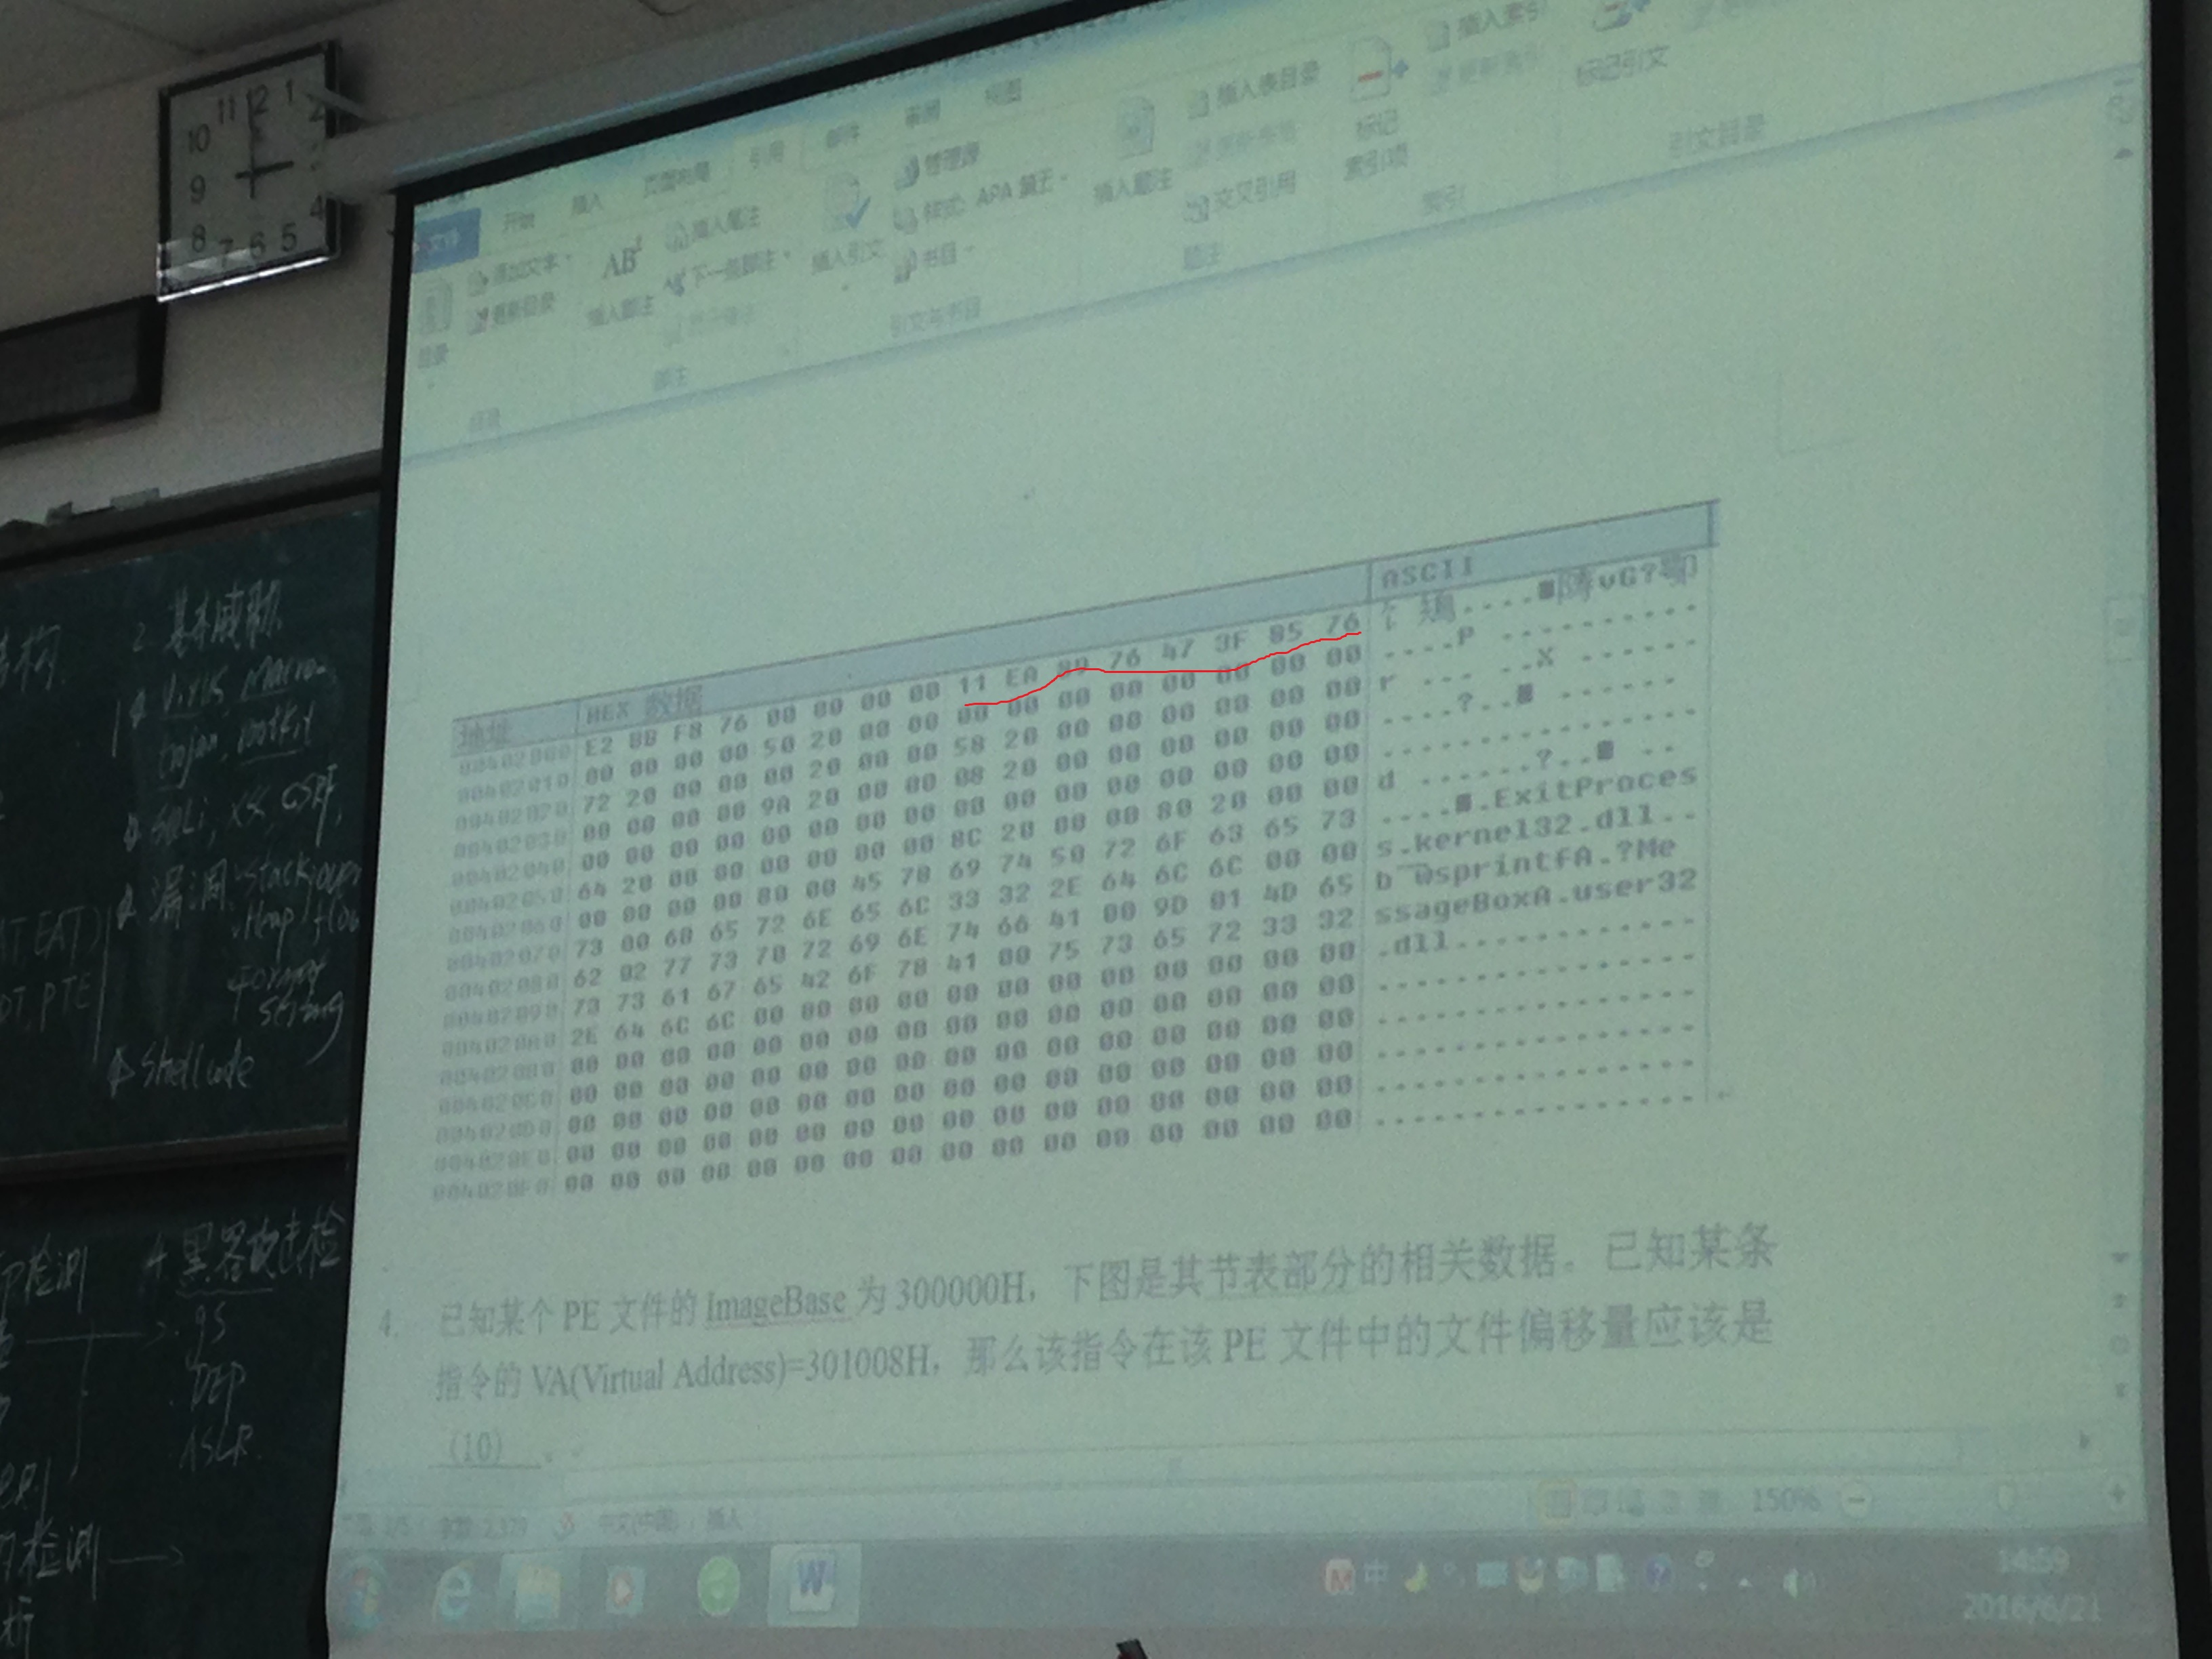
\includegraphics[width=0.6\textwidth]{6}
\end{figure}

尝试查找文件中是否存在 code cave,也就是找到 nop 最多的位置,发现没有。于是我们考虑用新增节的方式实现,一开始,我们想通过 int 80 中断的调用添加字符串的打印,但是在 bochs 运行中无法调用很多的系统中断,所以考虑从原程序中含有的内容入手。我们干脆覆盖掉一些其他的代码进行注入。

可以看到在0x1778处有字符串hello

\begin{figure}[H]
\centering
%[width=0.8\textwidth]
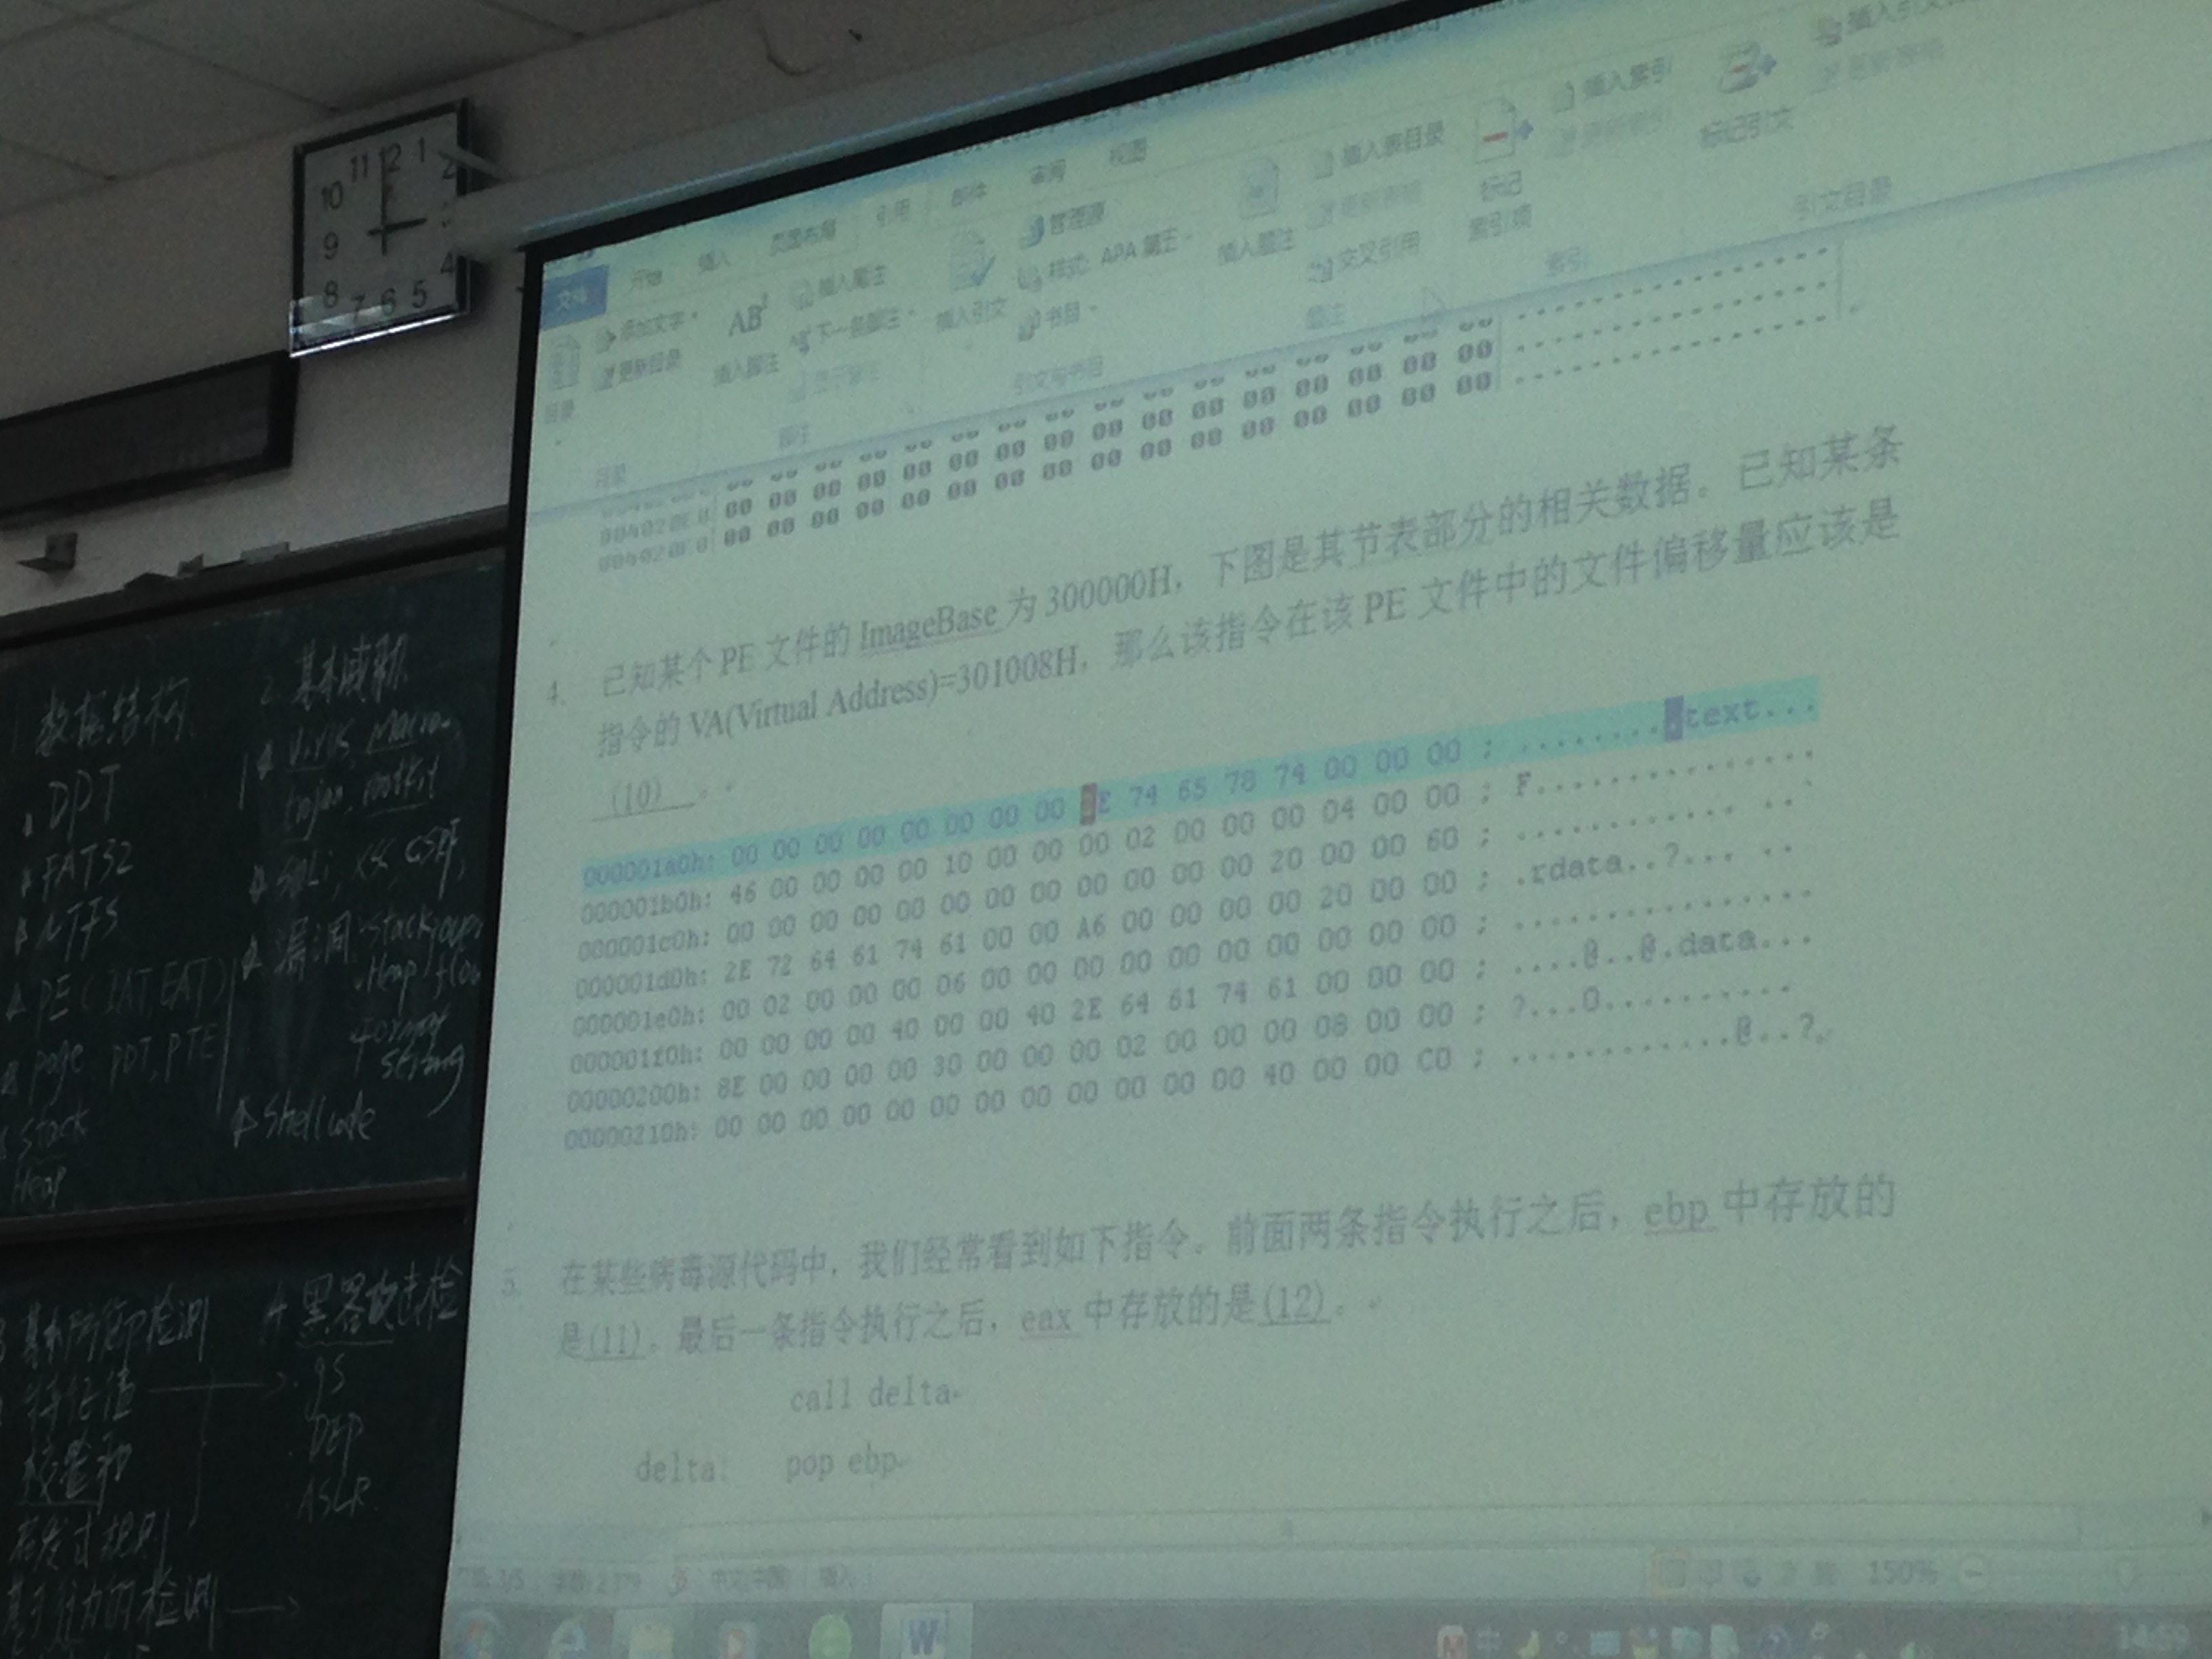
\includegraphics[width=0.8\textwidth]{7}
\end{figure}

在0x104e处有printf

\begin{figure}[H]
\centering
%[width=0.8\textwidth]
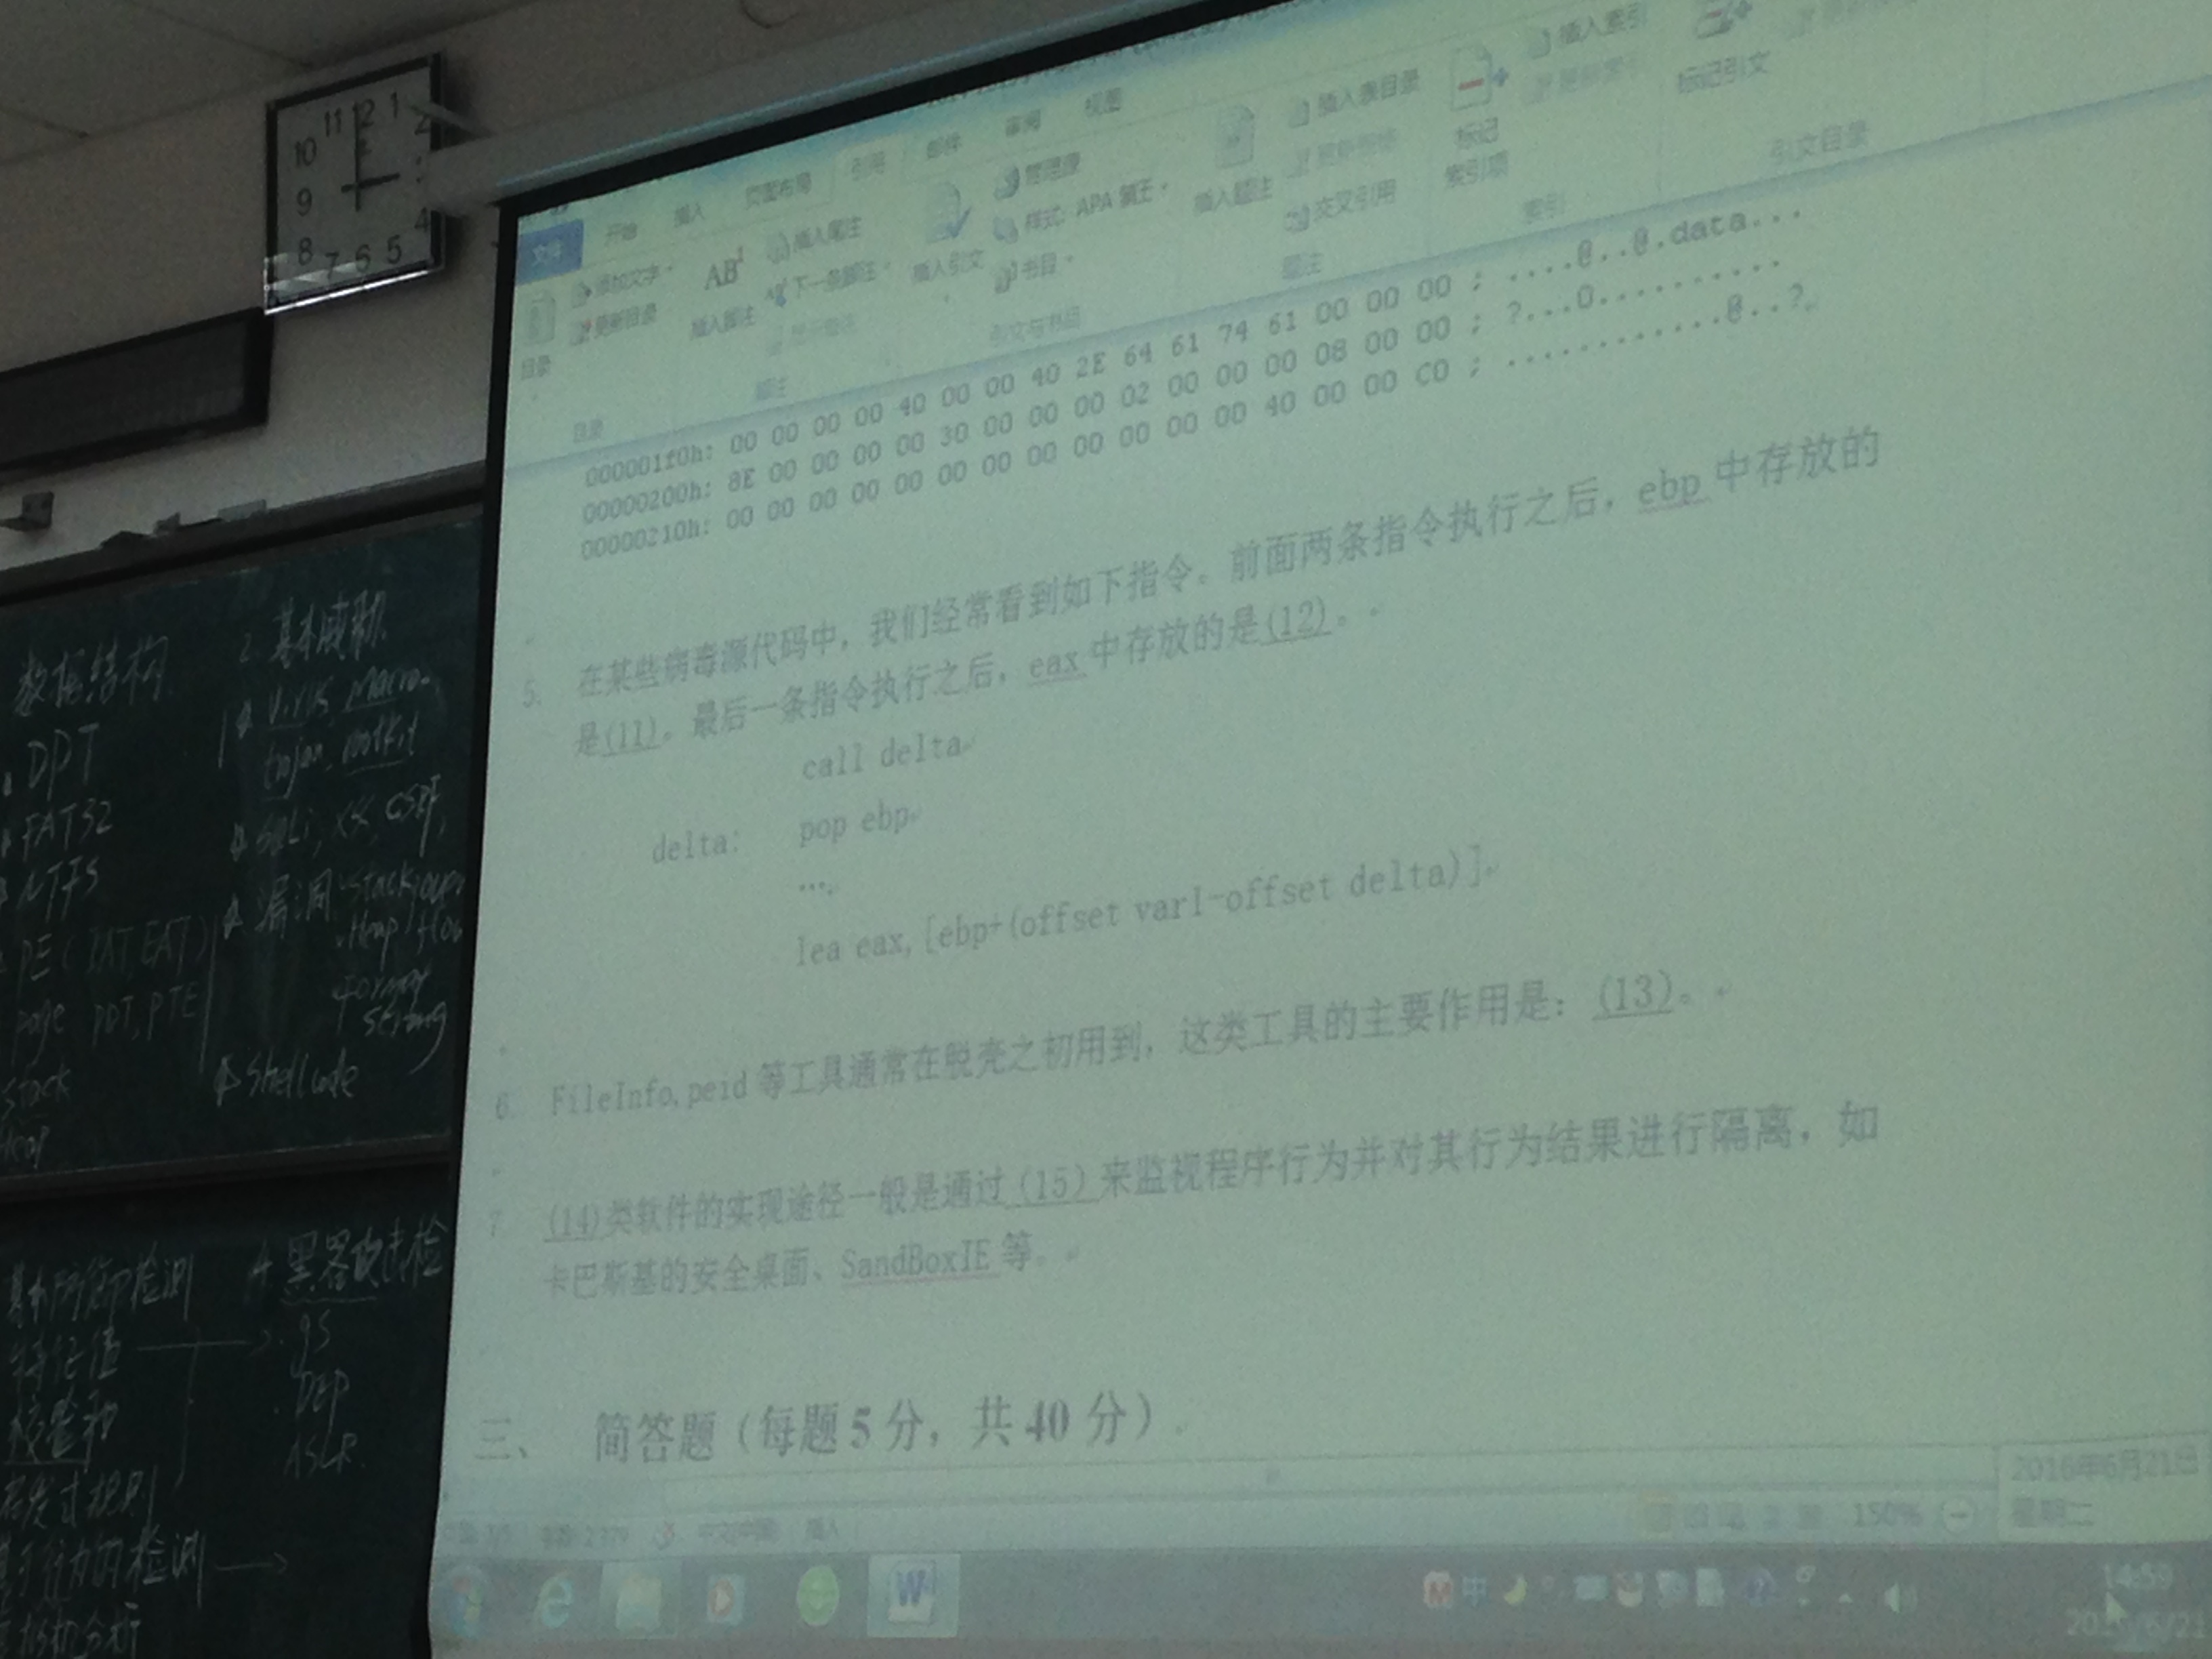
\includegraphics[width=0.8\textwidth]{8}
\end{figure}

我们可以复用这个输出,编写 shellcode 如下:
\begin{lstlisting}
char inject_code[] = {
	0х68, 0х78, 0x17, 0х00, 0х00,
 	0xe8, 0x20, 0х00, 0х00, 0х00
};
\end{lstlisting}

将文件指针指向对应的位置后,即可注入 shellcode。inject.c 代码如下:
\begin{lstlisting}
#include "stdio.h"
#include "string.h"
#include "elf.h"

#define PAGESIZE 4096

void cal_addr(int entry, int addr[]) {
    int temp = entry;
    int i;
    for (i = 0; i < 4; i++) {
        addr[i] = temp % 256;
        temp /= 256;
    }
}

void inject(char* elf_file) {
    printf("start to inject...\n");

    int old_entry;
    Elf32_Ehdr elf_ehdr;
    Elf32_Phdr elf_phdr;

    int old_file = open(elf_file, O_RDWR);
    read(old_file, &elf_ehdr, sizeof(Elf32_Ehdr));
    old_entry = elf_ehdr.e_entry;
    printf("old_entry: %x\n", old_entry);

    // Modify e_shoff of ELF Header,adding PAGESIZE
    // elf_ehdr.e_shoff += PAGESIZE;

    int i = 0;

    printf("Modifying the program header table...\n");
    // 读取并修改程序头部表
    close(old_file);
    old_file = open(elf_file, O_RDWR);
    char buffer[20000];
    read(old_file, buffer, elf_ehdr.e_phoff);
    read(old_file, &elf_phdr, sizeof(elf_phdr));

    printf("Inserting the injector...\n");
    // 插入注入程序
    close(old_file);
    insert(elf_ehdr, elf_file, old_entry);
}

void insert(Elf32_Ehdr elf_ehdr, char* elf_file, int old_entry) {
    // 程序的原始入口地址
    int old_entry_addr[4];
    cal_addr(old_entry, old_entry_addr);

    // printf("old_entry = 0x%x%x%x%x\n", old_entry_addr[3],old_entry_addr[2],old_entry_addr[1],old_entry_addr[0]);
    // 每一行对应一条汇编代码
    char inject_code[] = {
        0x68, 0x78, 0x17, 0x00, 0x00,
        0xe8, 0x20, 0x00, 0x00, 0x00,
	};
    int inject_size = sizeof(inject_code);

    // 防止注入代码太大
    if (inject_size > PAGESIZE) {
        printf("Injecting code is too big!\n");
        exit(0);
    }
    int old_file = open(elf_file, O_RDWR);
    u8 buffer[20000];
    read(old_file, buffer, 0x1024);
    write(old_file, inject_code, inject_size);
	close(old_file);
    old_file = open(elf_file, O_RDWR);
    read(old_file, buffer, 0x1024);
    read(old_file, buffer, 10);
    for (int i =0;i <10;i++) {
        printf("%x\n",buffer[i]);
    }

    printf("Finished!\n");
}

int main(int argc, char** argv) {
    if (argc != 2) {
        printf("inject <elf_filepath>\n");
        exit(0);
    }
    inject(argv[1]);
    return 0;
}
\end{lstlisting}

为实现对缓冲区的溢出攻击,编写函数如下。
\begin{lstlisting}
#include <stdio.h>
int i;
int *addr;

void test() { printf("pya, whx, thm, pzx"); }

void testat() {
	char buff[72] = {0};
	for (i = 0; i < 72; i++) {
    	buff[i] = 0;
	}

	for (; i < 72; i++) {
		buff[i] = 0;
	}

	addr = &buff[72];
	for (i = 0; i < 3; i++) {
		addr[i] = 0x1000;
	}
}

void main(int argc, char *argv[]) {
	testat();
}
\end{lstlisting}

调用testat函数后,栈底有返回地址,正常来说应该返回main函数。但是我们通过objdump得到test()函数的返回地址为0x1000,于是我们在向高地址填充地址0x1000,直到覆盖返回地址。那么会跳转到test()函数中输出我们想要的信息。

这种方式的栈溢出模拟了代码在代码段中的情况,但更多时候是通过产生shellcode将代码放入堆栈段中并跳转到堆栈运行,下面进行第二种方式的攻击演示:

\begin{itemize}
	\item 首先将代码通过objdump进行反汇编,由于printf在堆栈段中的地址需要重定位,因此这里使用简单的while循环来展示。
	\begin{figure}[H]
		\centering
		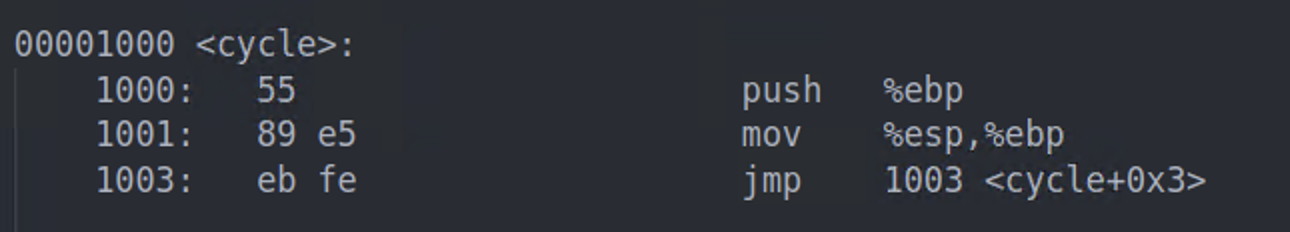
\includegraphics[width=0.8\textwidth]{whx10}
	\end{figure}
	\item 然后进入gdb将这段循环的代码转换为二进制文件
	\begin{lstlisting}
dump memory xxx.dump cycle cycle+5
	\end{lstlisting}
	\item 然后使用xxd过滤出shellcode,得到shellcode如下
	\begin{lstlisting}
xxd -i xxx.dump
	\end{lstlisting}
	\begin{figure}[H]
		\centering
		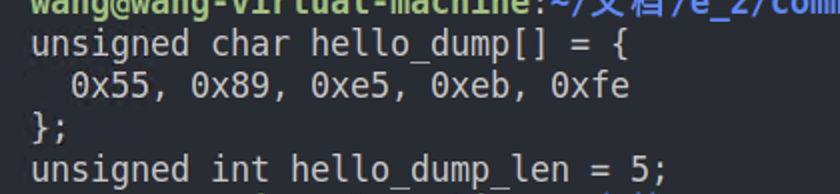
\includegraphics[width=0.6\textwidth]{whx11}
	\end{figure}
\end{itemize}


将这段代码放入shellcode\_dump[]数组中存放起来,然后使用下列代码:

\begin{lstlisting}
#include <stdio.h>
int i;
int* addr;

unsigned char shellcode_dump[] = {
    0x55, 0x89, 0xe5, 0xeb, 0xfe
};

void testat() {
	char buff[72] = {0};
	for (i = 0; i < 72; i++) {
		if (0 == shellcode_dump[i])
			break;
		buff[i] = shellcode_dump[i];
	}

	for (; i < 72; i++) {
		buff[i] = 0;
	}

	addr = &buff[72];

	for (i = 0; i < 6; i++) {
		addr[i] = buff;
	}
}

void main(int argc, char* argv[]) {
	testat();
}
\end{lstlisting}

这段代码会将原本函数返回地址覆盖为buff的初始地址,而buff已经被填入了shellcode,因此会不断执行在栈区循环。


\subsection{Part B 任务二}
在对可执行文件进行完整性验证这一部分,我们采用密码学算法AES进行可信防护。正如之前提到的,操作系统会先将指定的编译链接后的可执行文件打包 成一个 tar 包 inst.tar,再用工具 dd 写入磁盘的某段特定扇区。

在启动系统时,mkfs 会在文件系统中建立一个新文件 cmd.tar,并将其 inode 中的 i\_start\_sect 字段设置为 inst.tar 所在的扇区号。在初始化的时候会将 cmd.tar解包,把其中包含的文件都存入文件系统。 从理论上分析,我们应当在可执行文件打包成 inst.tar 之前,对可执行文件计算得到校验值,存放在操作系统的全局变量中。但因为在实验中,文件压缩操作是在 Makefile 中完成的,而且整个过程没有与外界的交互,即文件在 被解压之前都是处于原始安全的状态,为了方便起见,我们选择在解包的时候对 文件进行第一次的校验值计算,获得标志信息。

当某个子进程想执行某个文件时,通过文件名在文件系统中找到该文件,获 得文件的校验值,并与存放的校验值进行对比,如果不同说明文件已经被篡 改,不能执行;否则表示文件没有被篡改并继续打开执行。

我们首先把AES算法放入到lib文件夹,作为一个库函数。因为校验值在系统中需要有存放的位置,我们在头文件 proc.h 中定义了一个 结构体 check\_t,其中包含了三个成员:filename、byteCount 和 checkNum,分别代 表了文件名、文件大小(文件字节数)和校验值。

\begin{lstlisting}
struct check_t {
    char filename[32];
    int byteCount;
    u32 checkNum;
};
\end{lstlisting}


同时,在头文件 global.h 中定义了 check 结构体数组 check\_table,用来存放 所有文件的相关信息。

\begin{lstlisting}
PUBLIC	struct check_t	check_table[NR_CHECKFILES];
\end{lstlisting}

在 kenel/main.c 中,Init 函数调用了 untar 函数,我们将校验值计算的过程放入 untar 中。代码含义见注释。

\begin{lstlisting}
	// 记录了check_table的下标
    int check_count = 0;
    while (1) {
        read(fd, buf, SECTOR_SIZE);
        if (buf[0] == 0)
            break;

        struct posix_tar_header* phdr = (struct posix_tar_header*)buf;

        /* calculate the file size */
        char* p = phdr->size;
        int f_len = 0;
        while (*p)
            f_len = (f_len * 8) + (*p++ - '0'); /* octal */

        // FINISHED: untar first, than compute checksum!
        // bytes_left记录了还剩多少字节没有读取
        int bytes_left = f_len;
        // fout是写入到oranges中的文件句柄
        int fdout = open(phdr->name, O_CREAT | O_RDWR);
        if (fdout == -1) {
            printf("    failed to extract file: %s\n", phdr->name);
            printf(" aborted]");
            return;
        }

        printf("    %s (%d bytes)", phdr->name, f_len);
        char temp_name[32];
        strcpy(temp_name, phdr->name);
        while (bytes_left) {
        	// 一块一块读取文件内容到buf
            int iobytes = min(chunk, bytes_left);
            read(fd, buf,
                 ((iobytes - 1) / SECTOR_SIZE + 1) * SECTOR_SIZE);
            write(fdout, buf, iobytes);
            bytes_left -= iobytes;
        }
        close(fdout);

        if (strcmp(temp_name, "kernel.bin") != 0) {
        	// 把文件名字复制到check_table中
            strcpy((check_table + check_count)->filename, temp_name);
            // 把文件大小也放入check_table中
            check_table[check_count].byteCount = f_len;
            // 通过check函数计算校验值放入checkNum中
            check_table[check_count].checkNum = check((check_table + check_count)->filename, f_len);
            printf(" (checkNum = %d)\n", check_table[check_count].checkNum);
            check_count = check_count + 1;
        } else {
            printf("\n");
        }
    }
\end{lstlisting}

接下来我们看看checkh函数的具体实现:
\begin{lstlisting}
PUBLIC u32 check(char* filename, int byteCount) {
    int hFile = open(filename, O_RDWR);
    if (hFile < 0) {
        return -1;
    }

    u8 plaintext[16] = {0};
    u8 ciphertext[16] = {0};
    u32 key[4] = {0x12345678, 0x20193021, 0x40023201, 0x93021400};
    u32 current_checkSum = 0;

    // FINISHED: 一块一块读,加快check速度
    u8 buffer[byteCount];
    read(hFile, buffer, byteCount);
    for (int i = 0; i < byteCount; i++) {
        plaintext[i % 16] = buffer[i];
        if ((i % 16 == 0 && i != 0) || (i == byteCount - 1)) {
        	// 每读取完16字节后进行一次加密
            aes_enc(ciphertext, plaintext, key);
            for (int j = 0; j < 4; j++) {
            	// 我们用32bit作为一个checkSum,密文有128位
            	// 故密钥要循环四次计算checkSum
                u32 temp = ((u32)ciphertext[4 * j + 0] << 24) |
                           ((u32)ciphertext[4 * j + 1] << 16) |
                           ((u32)ciphertext[4 * j + 2] <<  8) |
                           ((u32)ciphertext[4 * j + 3] <<  0);
                current_checkSum ^= temp;
            }
        }
    }
    close(hFile);
    return current_checkSum;
}
\end{lstlisting}

完成上述步骤后,系统已经获得了各可执行文件的原始校验值,接下来就是在程序运行前对其进行再次的校验。获得了用户的键入后,会调用 execv 运行程序,但在运行之前需要验证校验值,从而判断是否能执行此文件。

\begin{lstlisting}
            else if (pid == 0) { /* child */
                p_proc_ready->p_flags = 1;
                block(p_proc_ready);

				/* 利用find_position函数找到该程序在check_table的位置 */
                int position = find_position(check_table, multi_argv[i][0]);
                /* 得到原始校验值 */
                u32 real_checkNum = check_table[position].checkNum;
                /* 对现在运行的程序进行校验值计算 */
                u32 now_checkNum = check(multi_argv[i][0], check_table[position].byteCount);
                /* 把这一句话取消注释就是关闭完整性验证
                 * 因为取消注释后now_checkNum 始终等于 real_checkNum
                 */
                // u32 now_checkNum = real_checkNum;

				/* 如果校验值相等则可以运行,否则打印文件被修改 */
                if (real_checkNum == now_checkNum) {
                    execv(multi_argv[i][0], multi_argv[i]);
                } else {
                    printf("This file has been changed!\n");
                }
            }
\end{lstlisting}

上面提到的find\_position也非常简单,就是遍历寻找位置:
\begin{lstlisting}
PUBLIC int find_position(struct check_t check_table[], char* filename) {
    for (int i = 0; i < NR_CHECKFILES; i++) {
        int flag = strcmp((check_table + i)->filename, filename);
        if (flag == 0) {
            return i;
        }
    }
    return -1;
}
\end{lstlisting}

除此,在本次实验中,实现的校验是在子进程创建后、执行前进行的, 相当于为执行函数 execv 加了一个保护壳。但这只能局部有效,如果有其他地方 调用 execv 函数,这时候是缺少验证的。因此,改进的方法就是直接把校验的过 程嵌入到 execv 函数体里,可以提高通用性。


\subsection{Part B 任务三}

在这个任务里,我们编写了一个软件中断,这个中断每过一定时间间隔触发,可以对进程表内的所有进程进行检查是否产生栈溢出,检查栈溢出的原理是根据内存的分布情况。

对于用户定义的程序,由于原本的OrangeOs中没有定义栈的区域,只给出了栈的上限,因此我们假定一个数据 0xF0000 作为栈的上限,栈位于 0xF0000 以上的位置,因此我们根据这条原则判断 proc 表中的用户进程的 eip 是否大于0xF0000来判断是否产生了栈溢出。

对于系统内核初始化的程序,由于其栈的区域为[task\_stack, task\_stack + STACK\_SIZE\_TOTAL],因此可以直接判定 eip 是否在栈区。

\begin{itemize}
	\item 下面是在proc.c中定义一个用来判断栈溢出的函数,这个函数对所有运行的进程进行检查
	\item 首先检查
	\begin{lstlisting}
PUBLIC int sys_checkstack()
{
	int i;
	/* 遍历进程表 */
	PROCESS *P = proc_table;
	for(i = 0; i < NR_TASKS + NR_PROCS; i++, P++)
	{
		if(P->p_flags == FREE_SLOT) //进程未使用
			continue;
		
		/* 对于在内核中初始化的程序检查其eip是否大于task_stack的地址 */
		else if(i < NR_TASKS + 4){
			if(P->regs.eip > (u32)task_stack){
				printf("detect stack overflow\n");
				assert(0);
			}
		}
		
		/* 对于用户的运行程序检查其eip是否大于0xF0000 */
		else if(P->regs.eip > 0xF0000)
			{
				//printf("CS=%x and SS=%x\n", P->regs.cs, P->regs.ss);
				printf("pid:%d, name:%s, detect stack overflow\n", i, P->name);
				P->regs.eip = exit;
			}
			//printf("name:: %s  CS:IP = %x : %x   SS:esp = %x::%x\n", P->name, P->regs.cs, P->regs.eip ,P->regs.ss, P->regs.esp);
	}
	return 1;
}	\end{lstlisting}
	\item 先在proto.h加入此函数的声明,并在global.c中将此函数添加到系统调用表中:
	\begin{figure}[H]
		\centering
		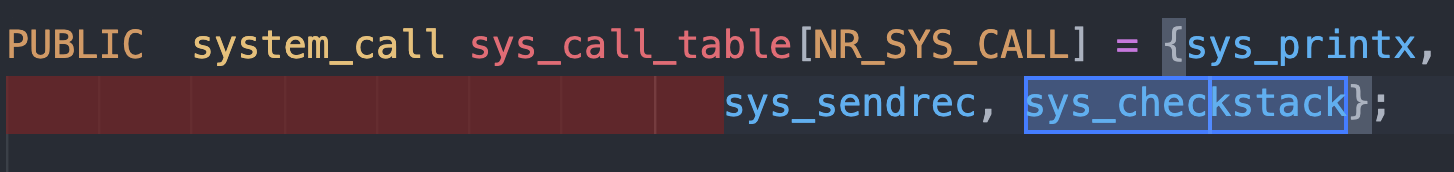
\includegraphics[width=0.8\textwidth]{whx15.png}
	\end{figure}
	
	\item 在syscall.asm中加入此系统调用:
	\begin{lstlisting}
	......
	_NR_checkstack	equ	2
	......
	global	checkstack
	......
	checkstack:
		mov eax, _NR_checkstack
		int INT_VECTOR_SYS_CALL
		ret
	\end{lstlisting}
	
	\item 最后在kernel/main.c的TextA进程中每隔一定时间间隔调用检查函数,在检查前需要延迟一段时间先让 INIT 函数完成初始化:
	\begin{lstlisting}[language=c]
	void TestA() {
    int k, i, j;
    int fd_stdin = open("/dev_tty1", O_RDWR); 
    assert(fd_stdin == 0);
    int fd_stdout = open("/dev_tty1", O_RDWR);
    assert(fd_stdout == 1);

    int check;
    for(k=0;k<100;k++){
            for(i=0;i<10;i++){
                for(j=0;j<10000;j++){}
            }
        }
    while(1){
    if(ticks % 200 == 0) // 等效于按照定时中断触发
        check = sys_checkstack();
    }   
}
	\end{lstlisting}
\end{itemize}

在这种检测方式下,我们认为只要eip不大于0xF0000就算合法,这是基于栈区往往在高地址而设置的。
这种防御手段仅能防御住部分将代码放在栈区执行的缓冲区溢出攻击。对于我们在任务一实现的栈溢出攻击而言,第一种情况,也就是通过栈溢出跳转到代码段中的函数入口执行,这种防御手段无法防御,这种攻击手段常见于绕过保护验证;但对于第二种攻击手段,也就是构造shellcode放入栈区等到溢出后执行的攻击可以进行防御。


\section{实验结果总结}

\subsection{准备工作}
首先每次都需要改一改bochsrc,需要把romimage和vgaromimage的位置改成自己电脑安装的位置:
\begin{figure}[H]
\centering
%[width=0.8\textwidth]
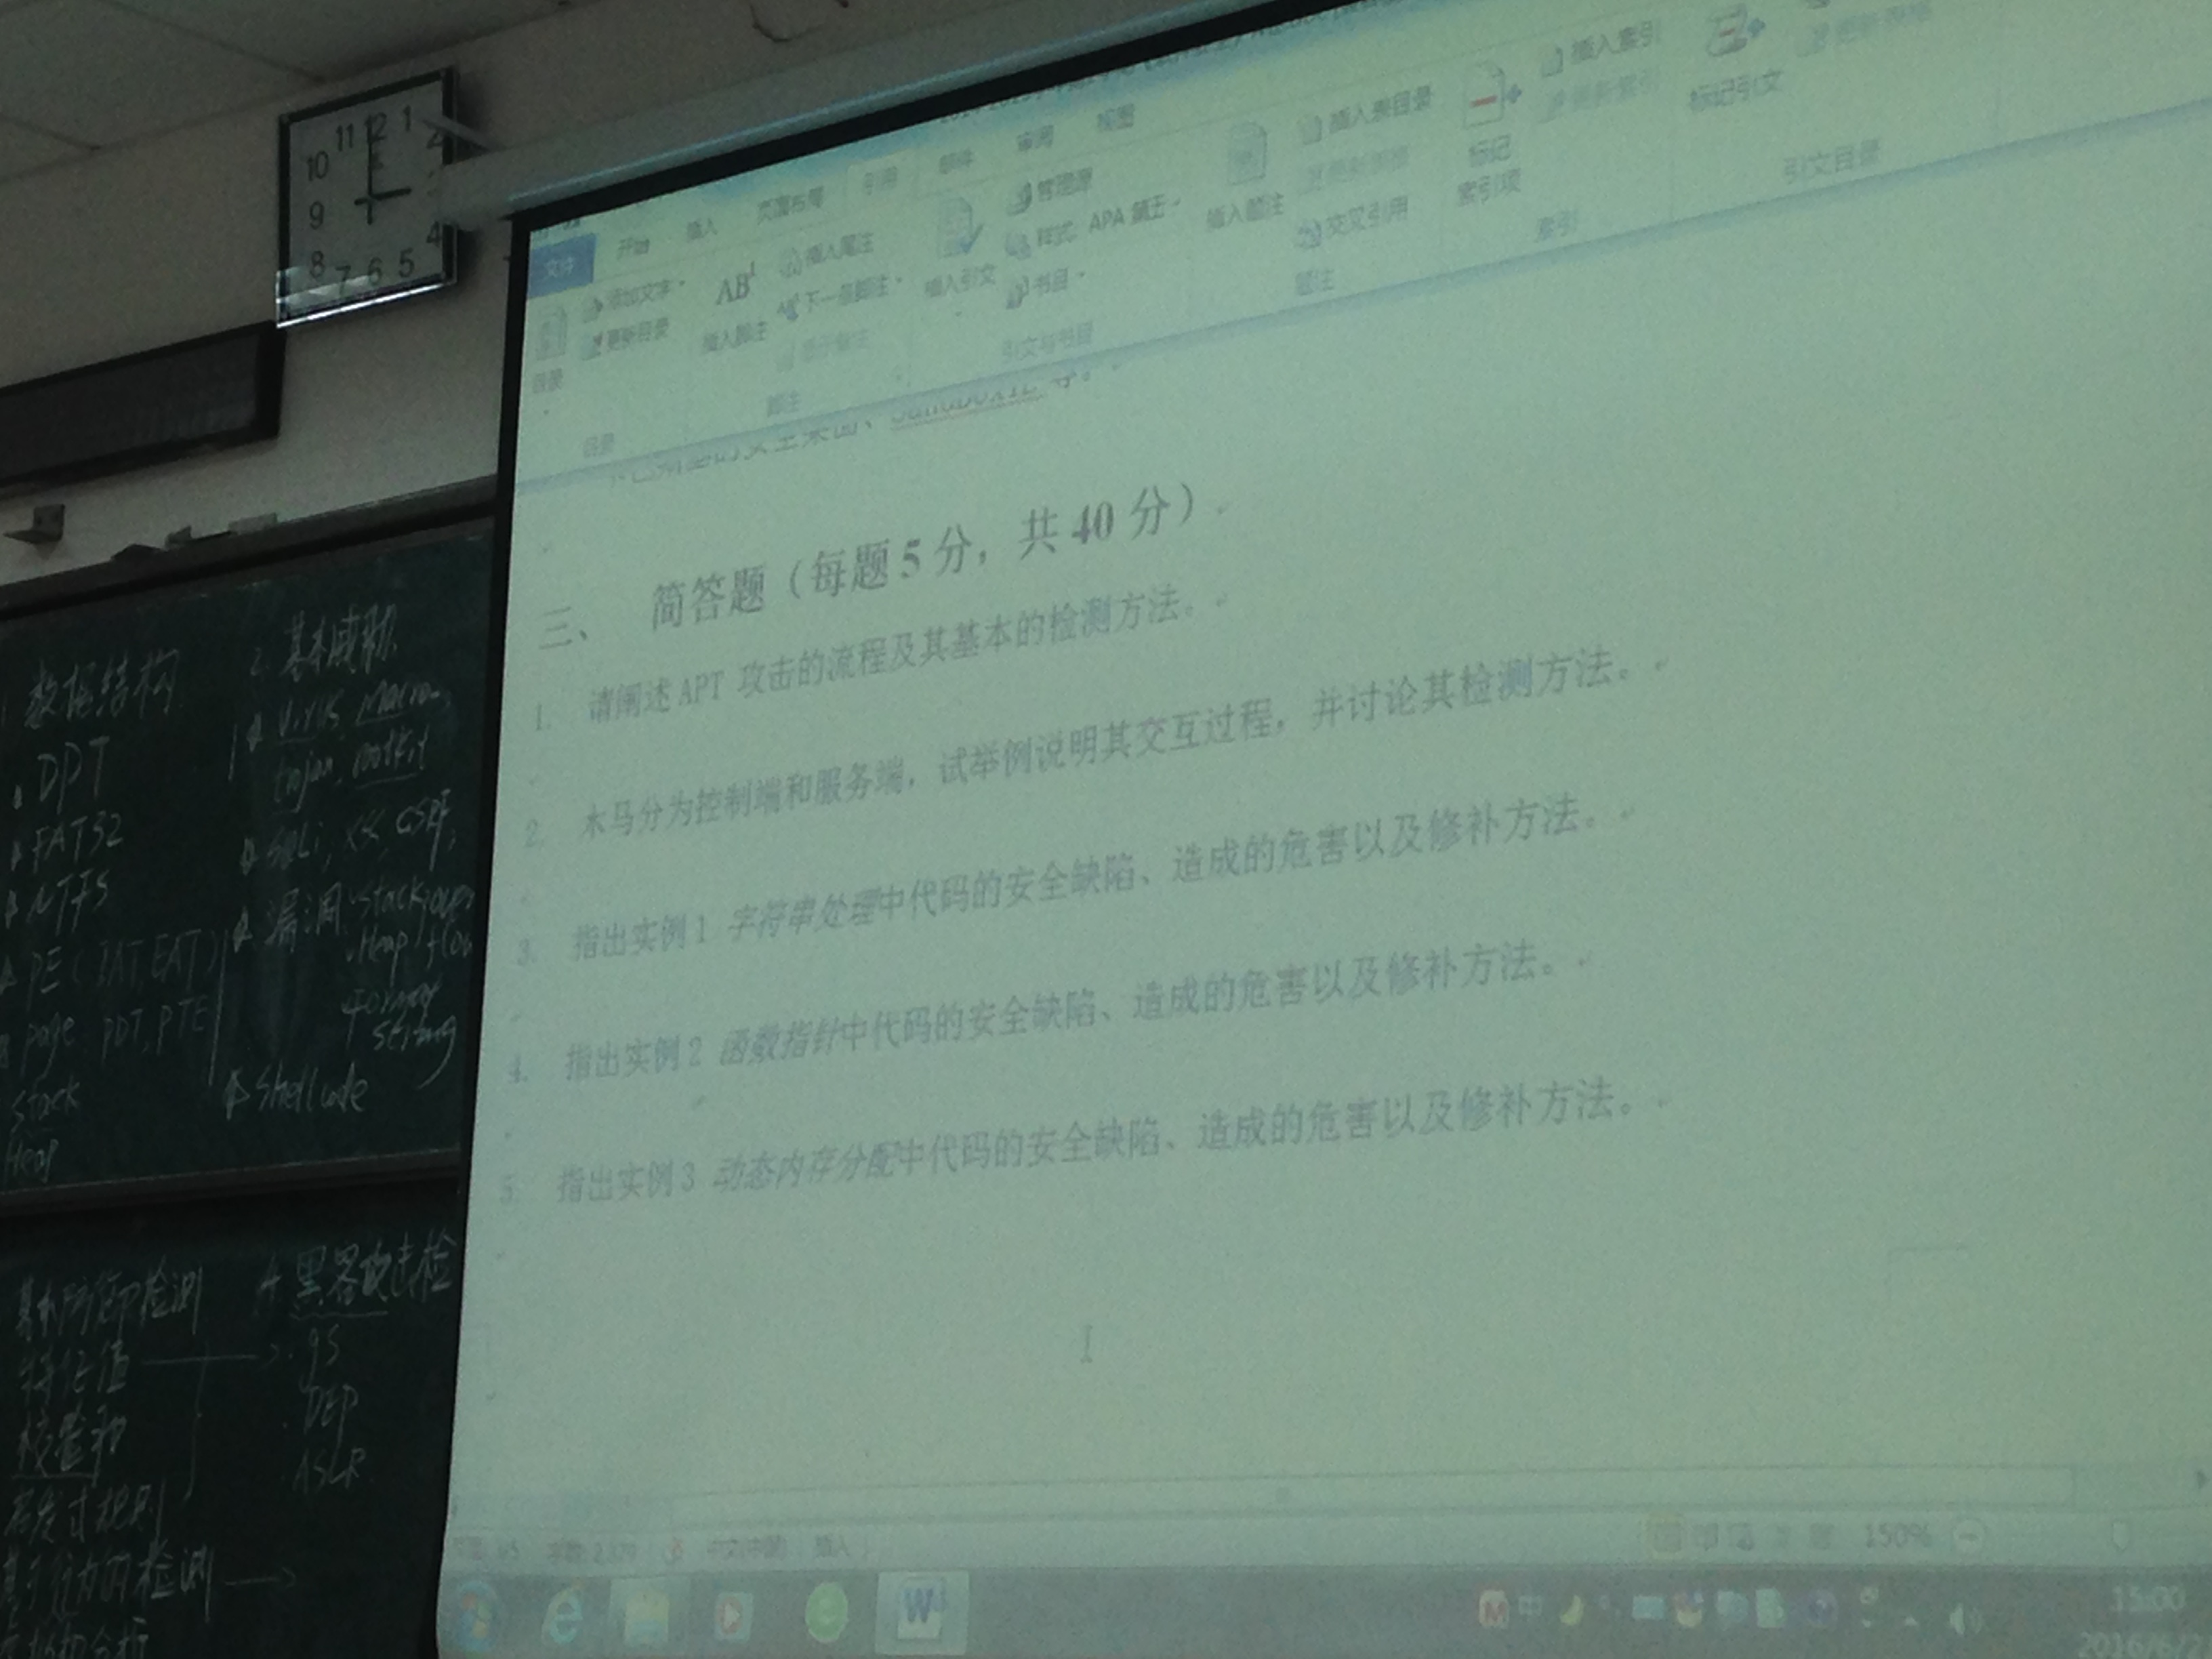
\includegraphics[width=0.8\textwidth]{9}
\end{figure}


makefile编译的时候要加上-fno-stack-protector,这个问题在之前的实验也出现过。

上面的修改好之后,第一次运行的时候卡住了,报错为HLT IF=0。在 kernel/proc.c 中,应该在进入 msg\_receive 函数后先关中断,在退出函数时(该函数有两个return退出)重新开中断。这是为了防止进程冲突,保护该过程不被中途停止。

\begin{figure}[H]
\centering
%[width=0.8\textwidth]
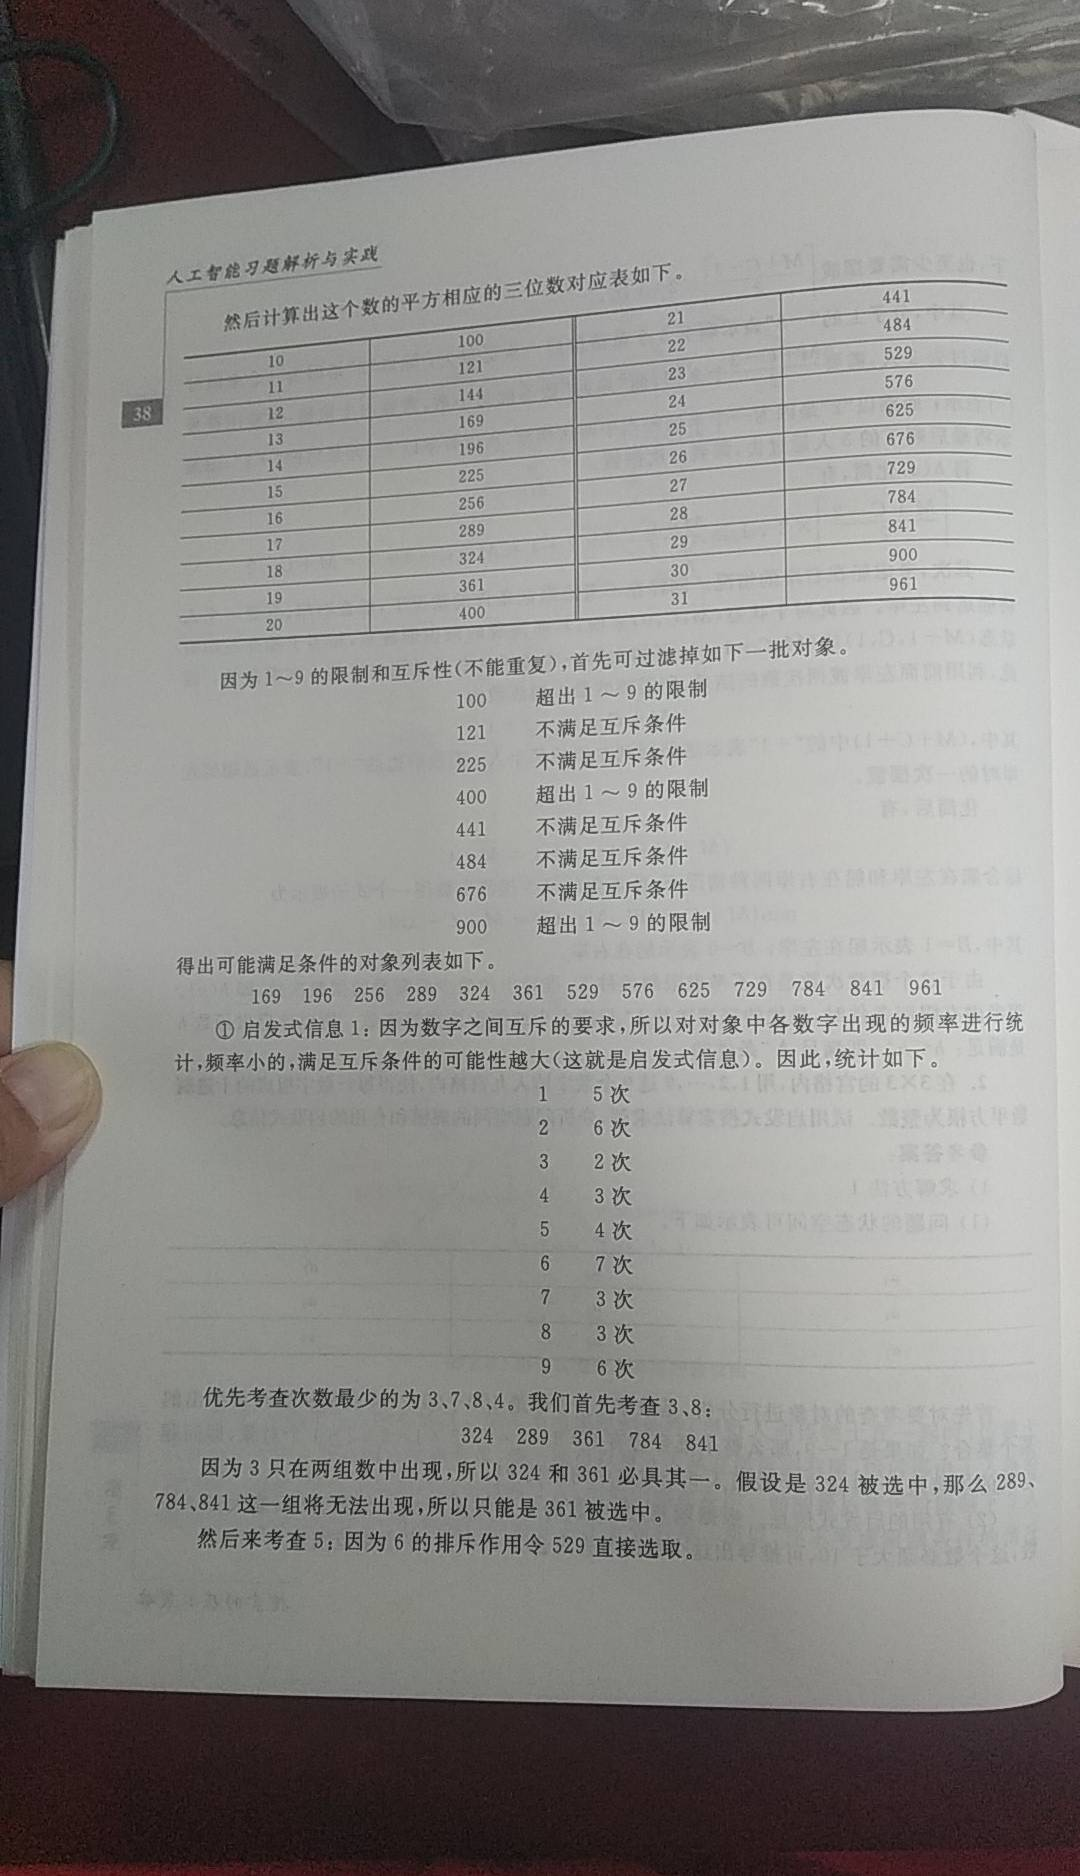
\includegraphics[width=0.8\textwidth]{10}
\end{figure}

最后需要在 kernel/tty.c 中,将切换 shell 的功能键 ALT 改为 CTRL。这是因为
ALT 在 ubuntu 中是特殊的功能键,所以我们用 CTRL 替换了该键。

\subsection{实验结果}

\subsubsection{Part A}
Part A 任务一实现了多级反馈调度算法,这里打印出了进程在三个队列中的排队情况,并且<>内包含了该进程剩余时间片。可以看到A-G进程首先都在1队列,然后A在第一队列运行了10个时间片后,剩余时间片从0x96变成0x8C,并且进入到第二个队列...

由于在第六章的代码中,所有进程都必须手工创建,也就是只能在0时刻的时候手动添加,所以最后输出的性能评价信息中提交时刻都是0。并且后面还输出了结束时间、响应时间和等待时间。通过理论计算验证,实际输出的时间和理论略有一点偏差。这是因为实际过程中,除了这些函数要消耗时钟,其他函数比如调度过程、切换过程等等都需要消耗少量时钟。

\begin{figure}[H]
\centering
%[width=0.8\textwidth]
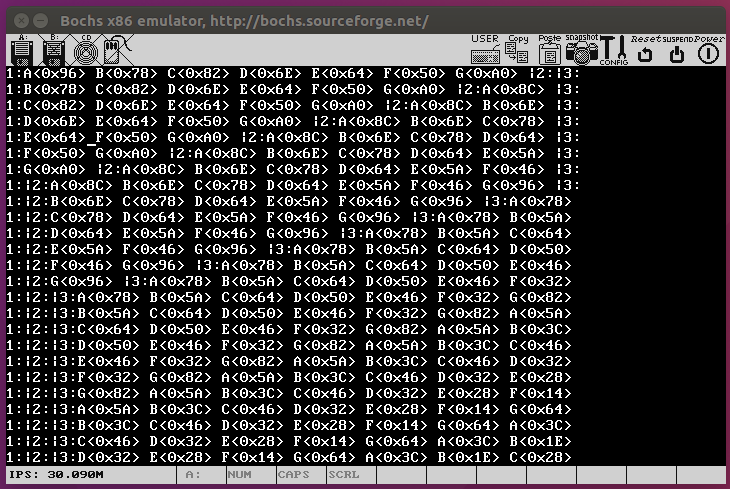
\includegraphics[width=0.8\textwidth]{21}
\end{figure}

\begin{figure}[H]
\centering
%[width=0.8\textwidth]
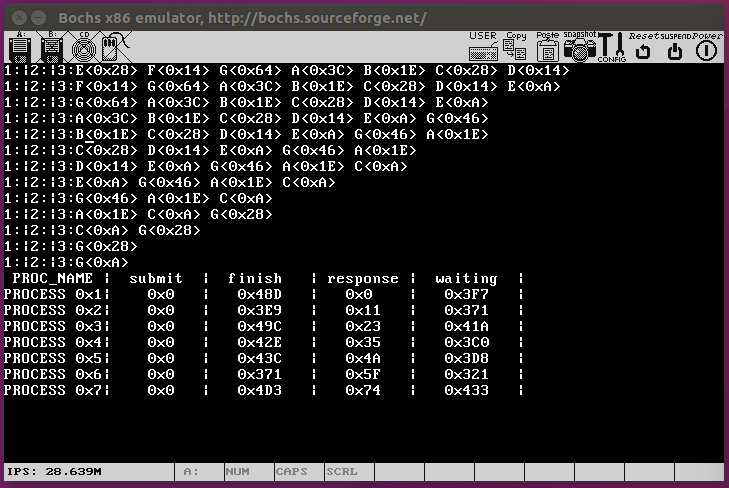
\includegraphics[width=0.8\textwidth]{22}
\end{figure}


Part A 任务二实现DES和AES算法,输入des -h和aes -h可以获得帮助信息。加解密如下图所示,可以看见我们成功实现了加解密。
\begin{figure}[H]
\centering
%[width=0.8\textwidth]
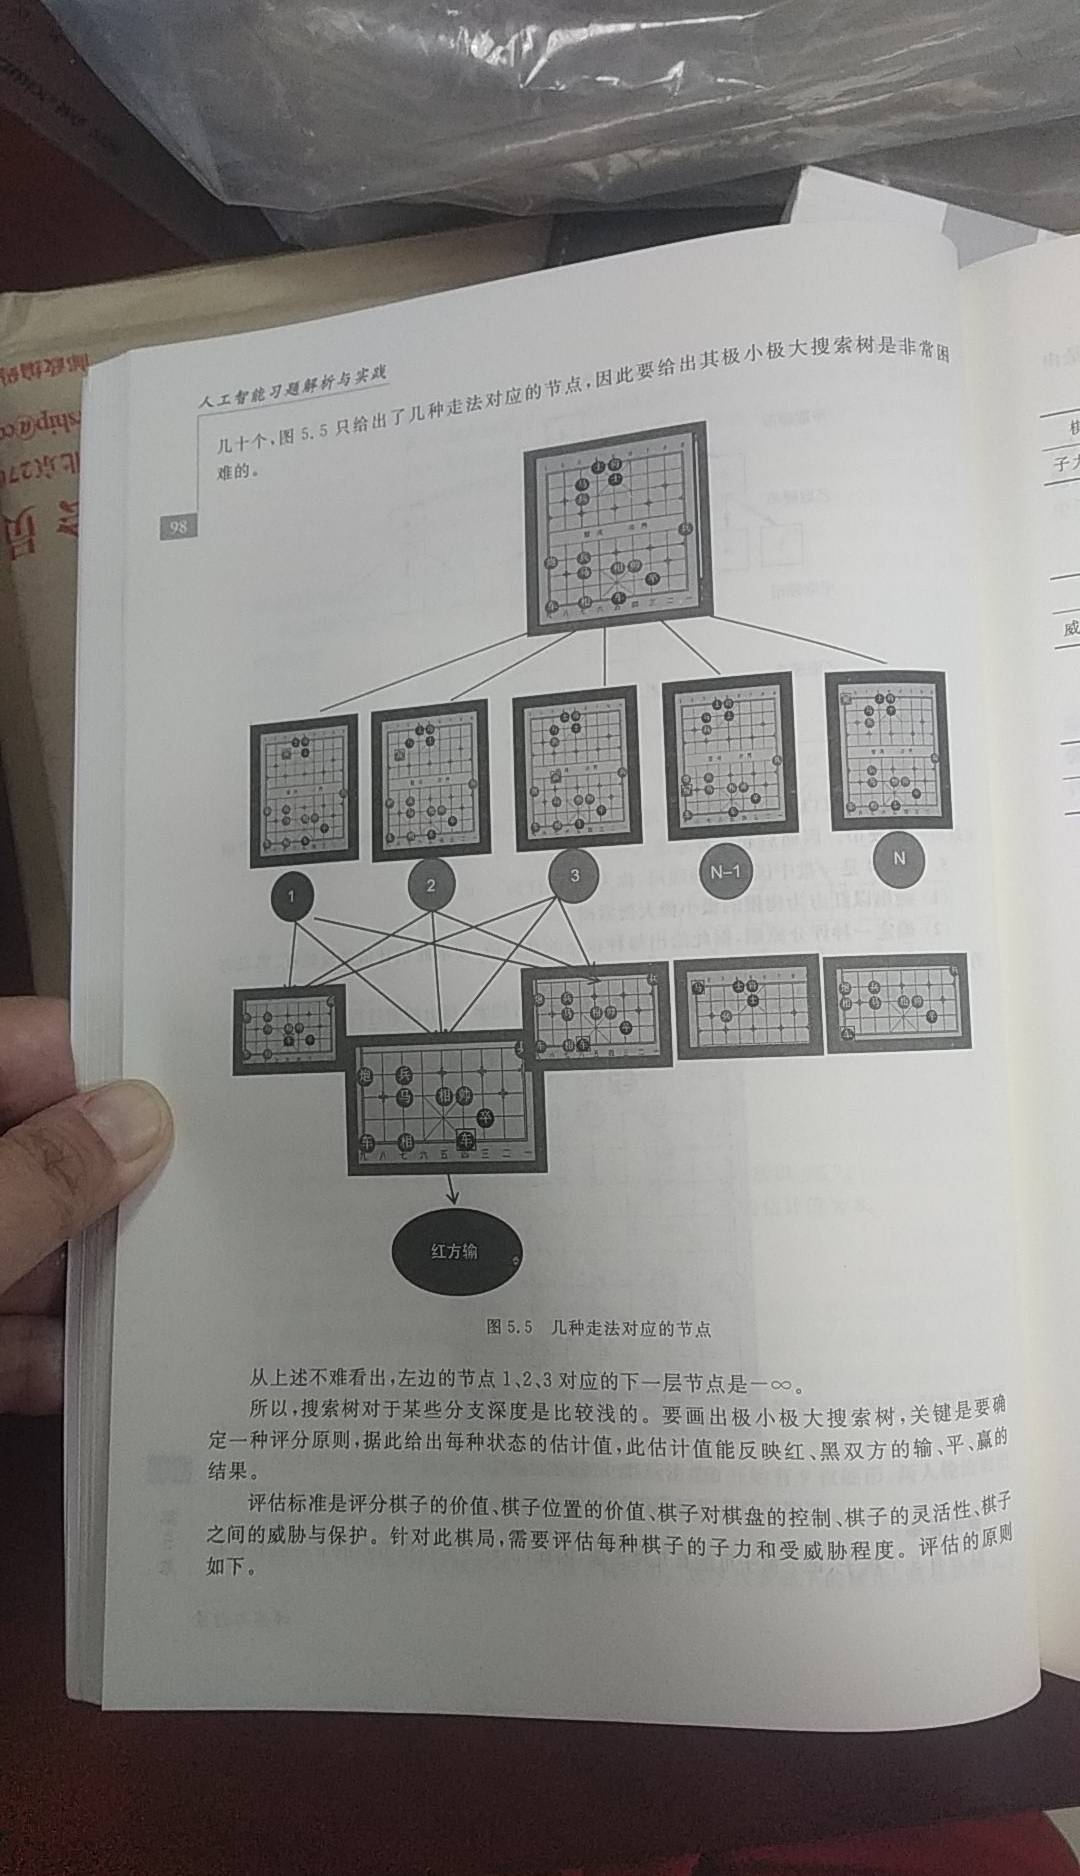
\includegraphics[width=0.8\textwidth]{23}
\end{figure}

Part A 任务二我们还实现了类似linux的ps命令,可以看到我们成功利用消息传递机制输出了进程信息:

\begin{figure}[H]
\centering
%[width=0.8\textwidth]
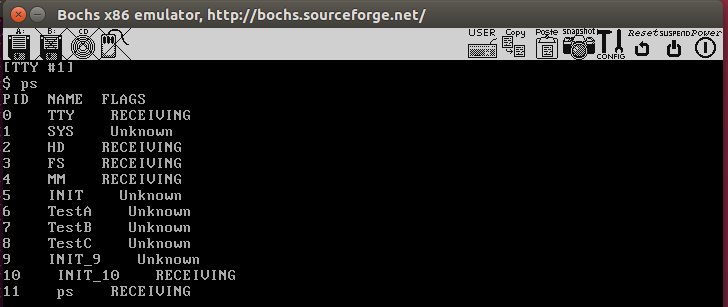
\includegraphics[width=0.8\textwidth]{30}
\end{figure}

Part A 任务三实现了shell多任务执行的支持。从下图可以看出,不管是两个任务还是三个任务,都可以成功运行。但是如果命令出错,无论在哪一个位置,都不会继续执行。同时为了展示我们所做的确实成功实现了多任务执行,也就是能够正常调度,我们编写了两个函数inf1和inf2,inf1无限循环输出a,inf2无限循环输出b,可以看到输出结果ab交叉输出,说明我们确实完成了多任务的支持。

\begin{figure}[H]
\centering
%[width=0.8\textwidth]
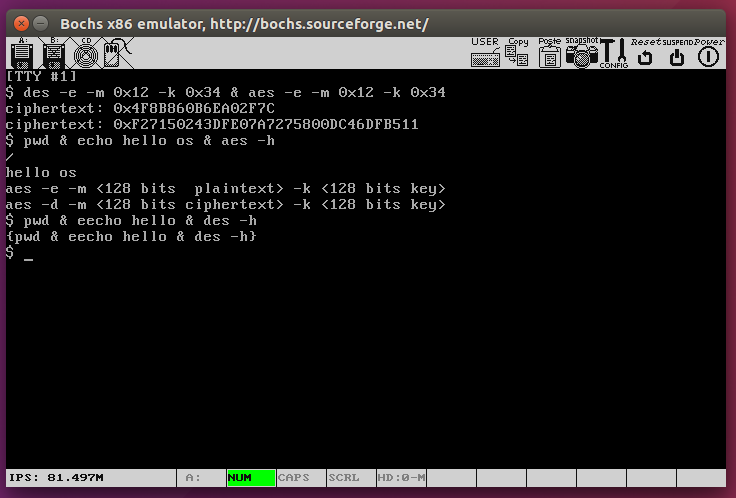
\includegraphics[width=0.8\textwidth]{24}
\end{figure}

\begin{figure}[H]
\centering
%[width=0.8\textwidth]
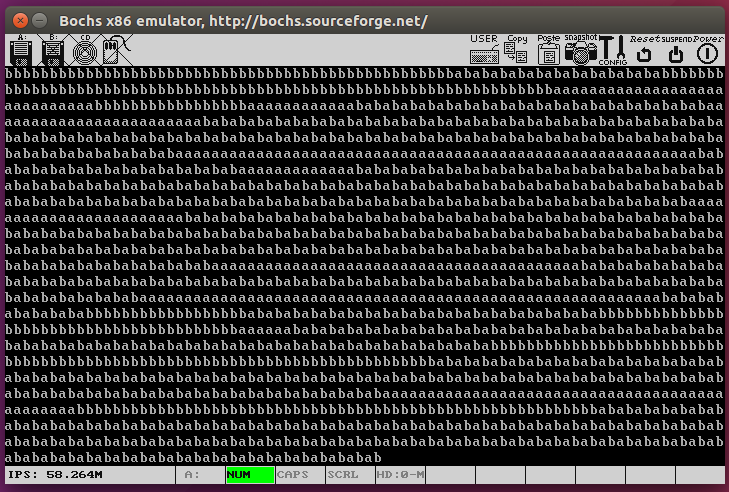
\includegraphics[width=0.7\textwidth]{25}
\end{figure}

Part A 任务四我们认为思路是这样做没有问题,但还是出现了许多bug并没有调通。

\subsubsection{Part B}
Part B 任务一第一个小任务是进行elf文件注入,由于我们完成了任务二的完整性检验,所以在进行该实验的时候我们需要去/kernel/main.c中341行取消注释,取消注释就是关闭完整性检验,注释这一行就是开启完整性检验。注入的结果如下,首先输出hello和我们小组成员名字;在注入时,保存old entry,修改program header table,然后进行注入,下面的数字是为了编写时调试方便输出的;注入完成后运行hello,可以发现这会会输出两个hello而不输出小组成员名字了,说明成功注入了代码。

\begin{figure}[H]
\centering
%[width=0.8\textwidth]
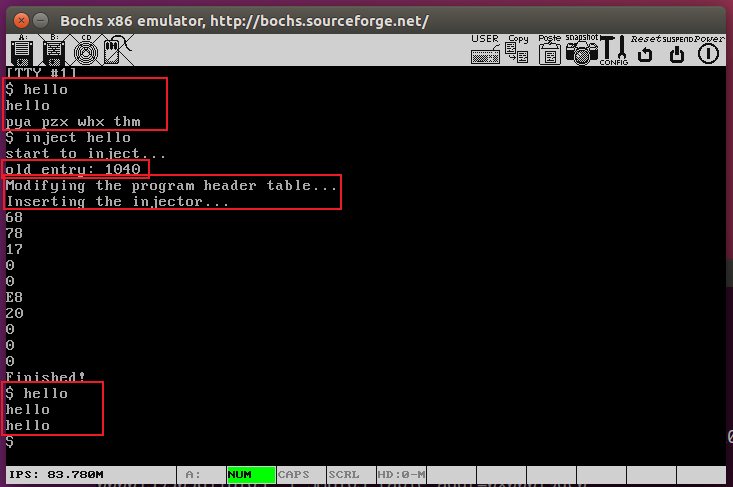
\includegraphics[width=0.7\textwidth]{26}
\end{figure}

Part B 任务一的缓冲区溢出部分我们有两个版本的代码。第一个是在代码段的缓冲区溢出,结果如下,我们可以看到成功返回到test()函数然后执行了其中的printf代码:

\begin{figure}[H]
\centering
%[width=0.8\textwidth]
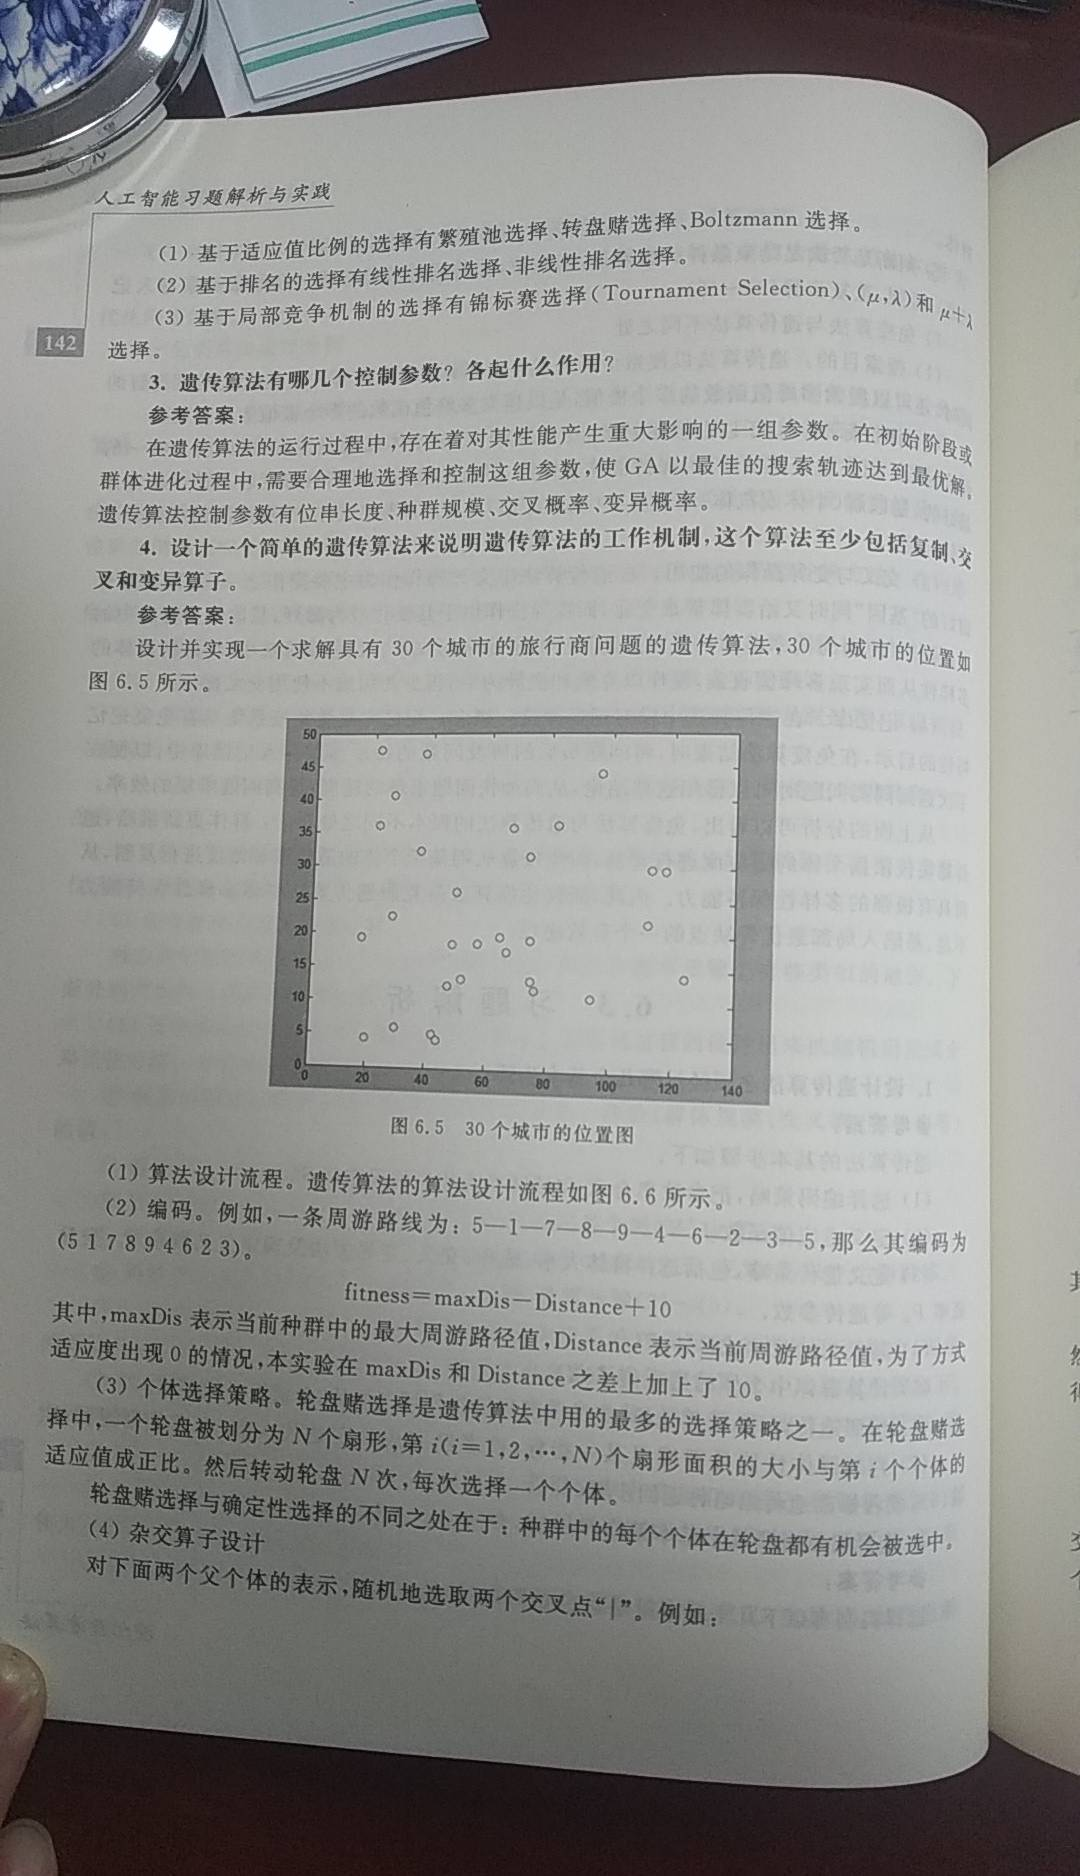
\includegraphics[width=0.8\textwidth]{27}
\end{figure}

第二个时堆栈段的缓冲区溢出,这段代码会将原本函数返回地址覆盖为buff的初始地址,而buff已经被填入了shellcode,因此会不断执行在栈区循环。下面是实验结果:

\begin{itemize}
\begin{figure}[H]
	\centering
	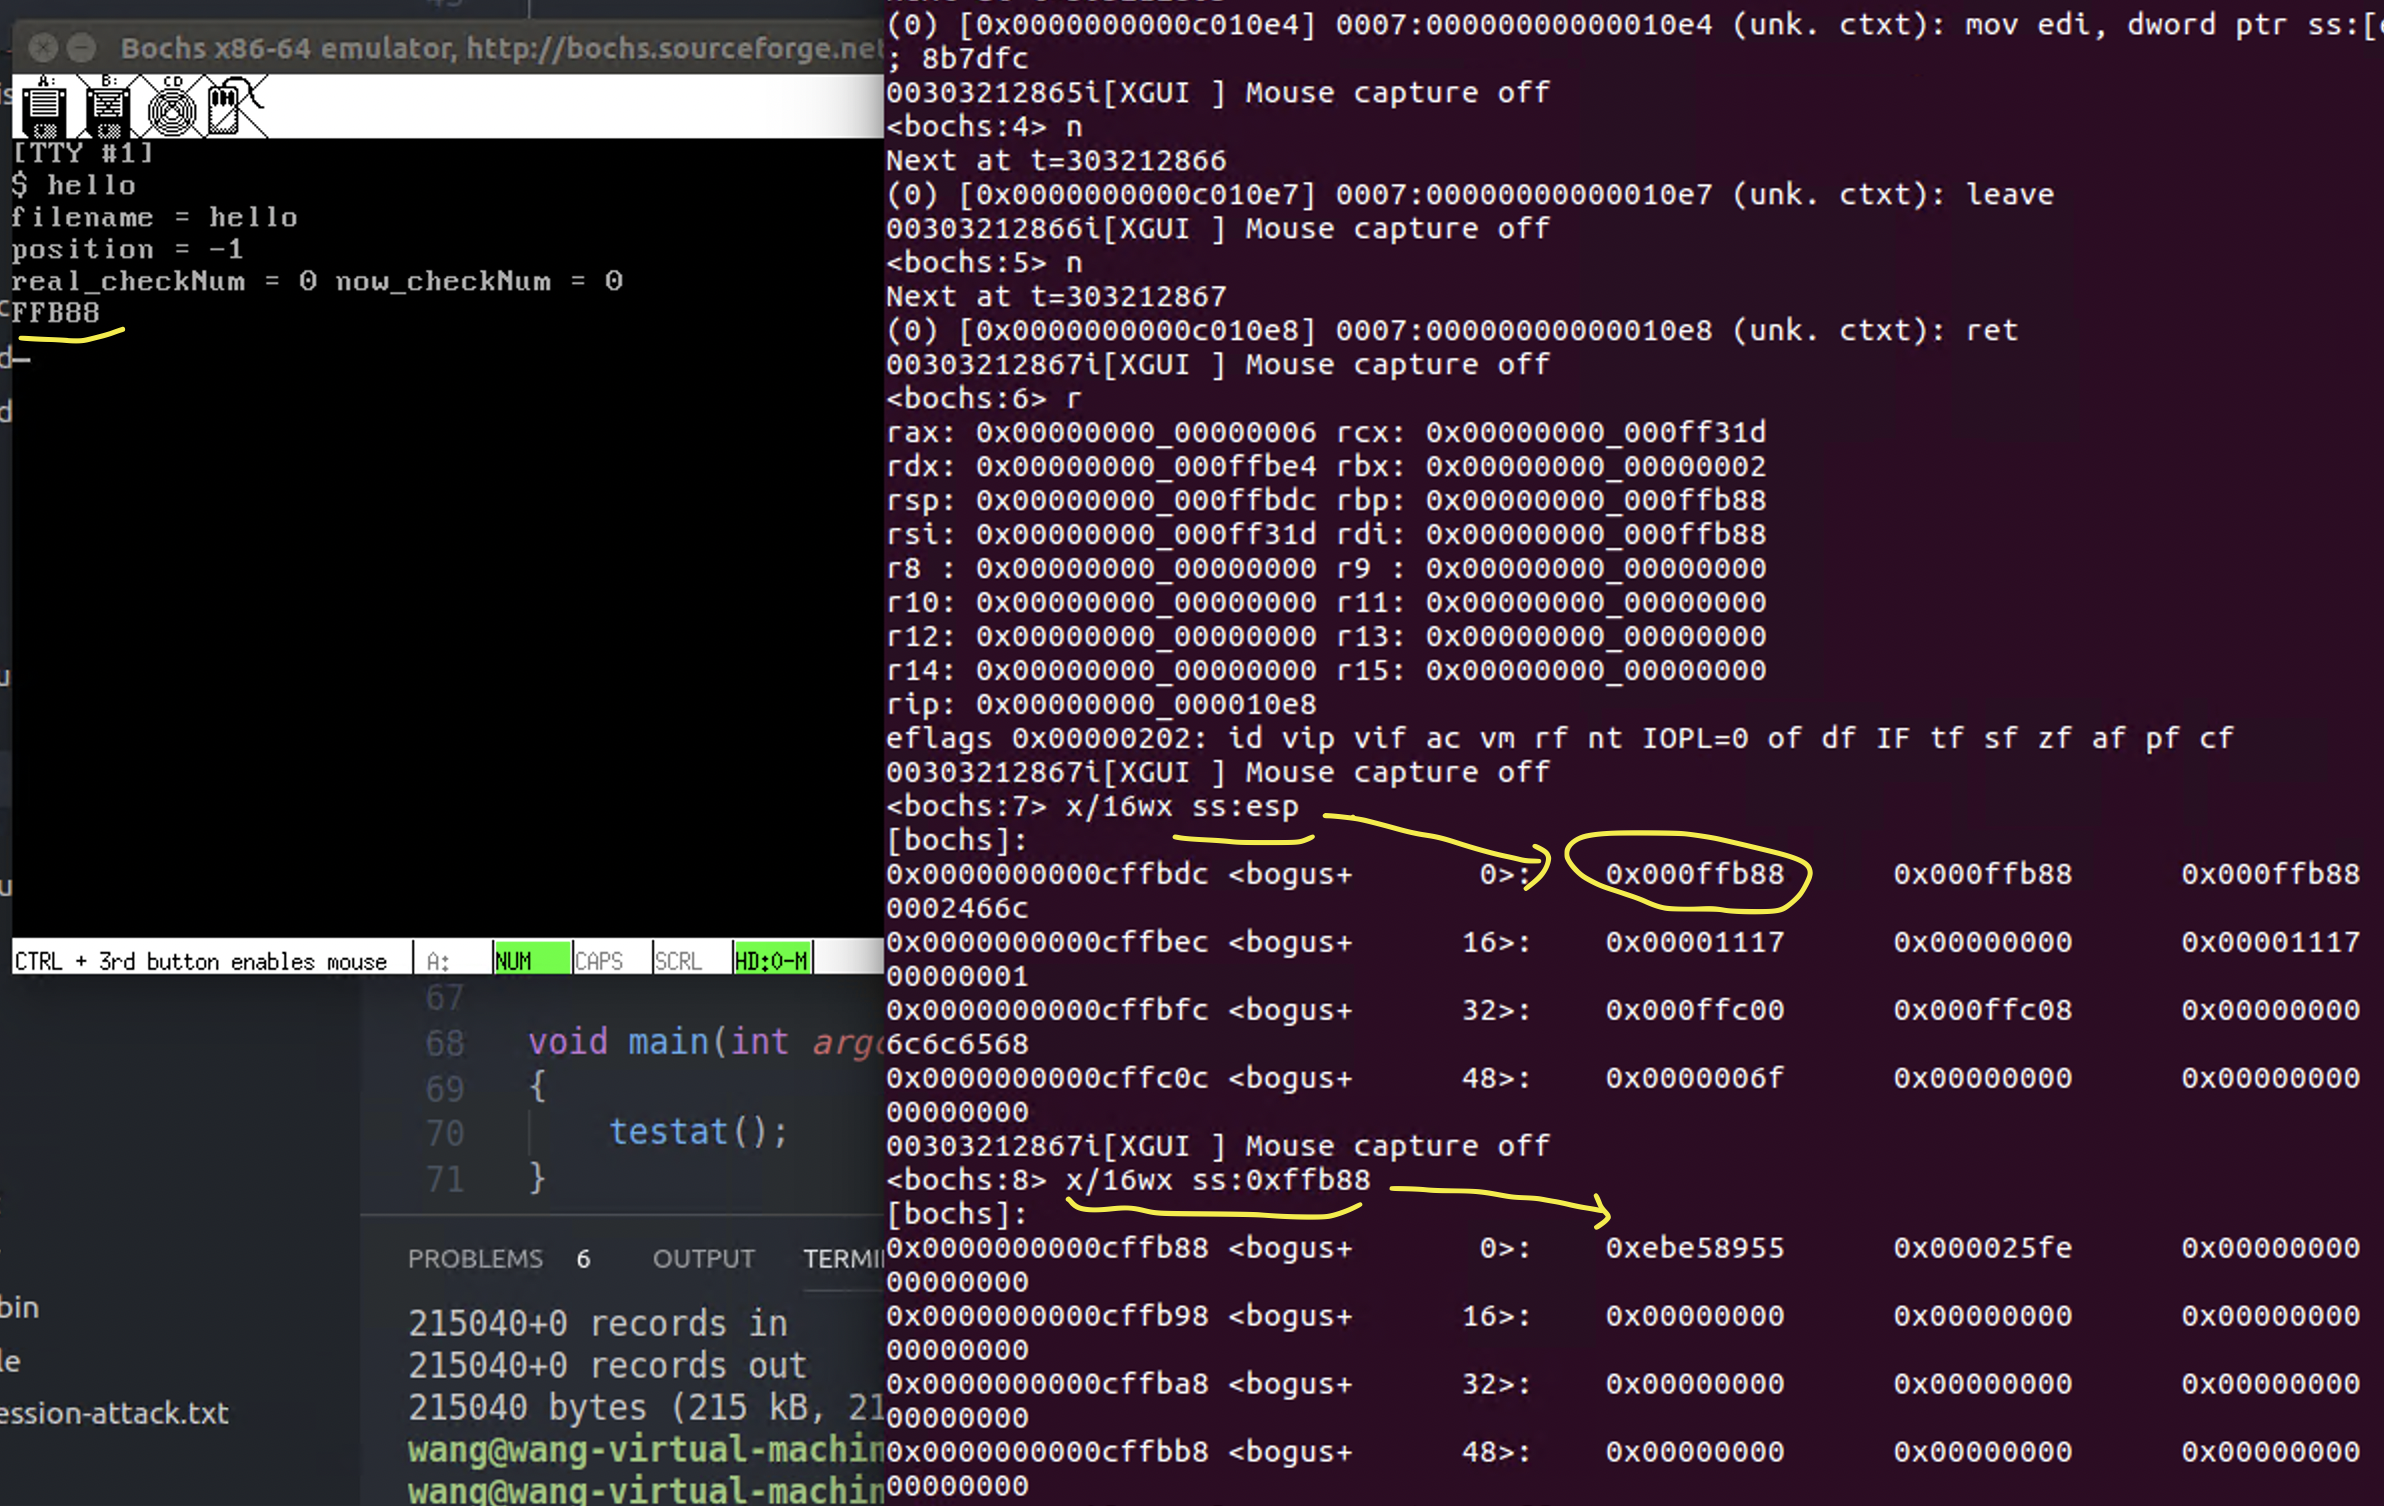
\includegraphics[width=0.8\textwidth]{whx12}
\end{figure}
	\item 在返回点下断点查看堆栈的返回情况,可以看见在返回点处ss:esp与程序输出的数组buff的地址相等,这说明程序下一步将会返回到buff的地址处。查看ss:esp处的内容,发现已经是我们填入的while循环的机器码,因此程序下一步进入死循环。
	\begin{figure}[H]
		\centering
		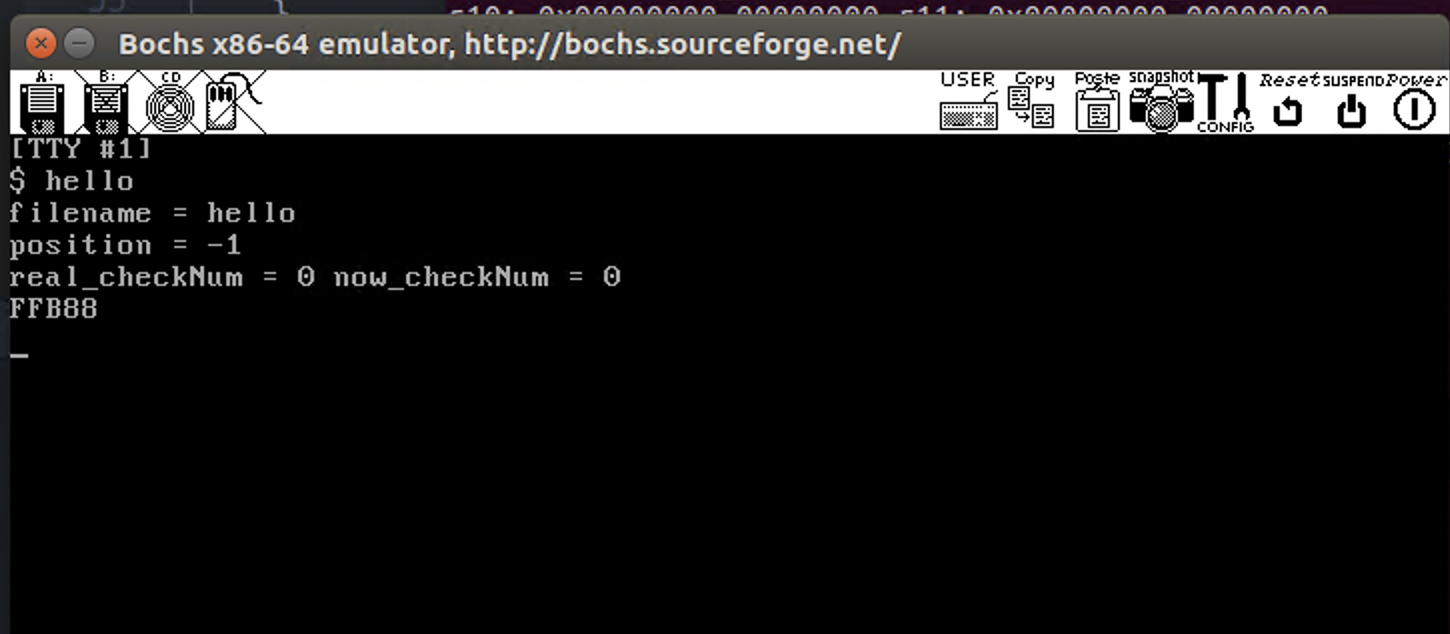
\includegraphics[width=0.6\textwidth]{whx14}
	\end{figure}
\end{itemize}

Part B 任务二要在运行命令前对可执行文件做一次完整性检验,我们注释掉/kernel/main.c中341行即可开启完整性检验。首先可以看到os刚启动的过程会计算校验码。随后运行hello命令可以成功运行,也就是此时校验通过。但是当注入后再次运行,会提示该文件已被修改,也就是此时运行在此计算校验码和os刚启动时保存的校验码不一致。

\begin{figure}[H]
\centering
%[width=0.8\textwidth]
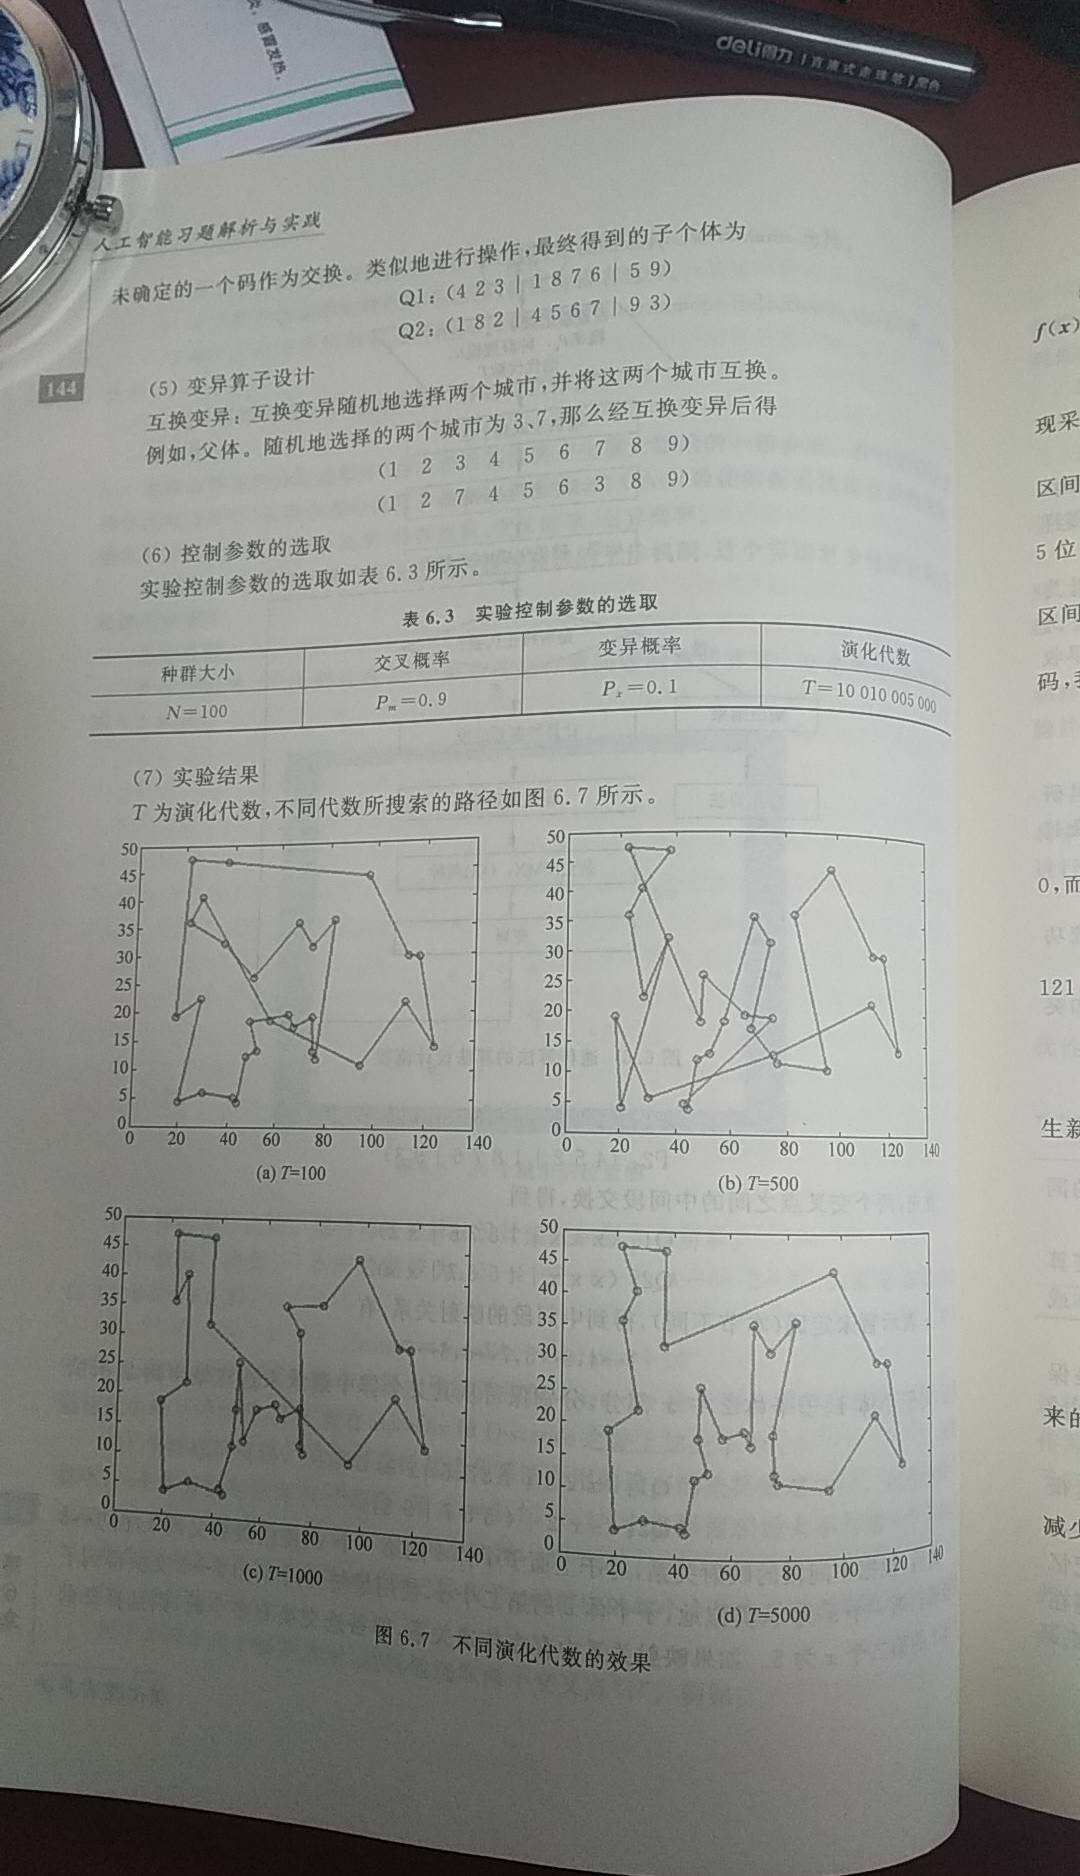
\includegraphics[width=0.8\textwidth]{29}
\end{figure}

\begin{figure}[H]
\centering
%[width=0.8\textwidth]
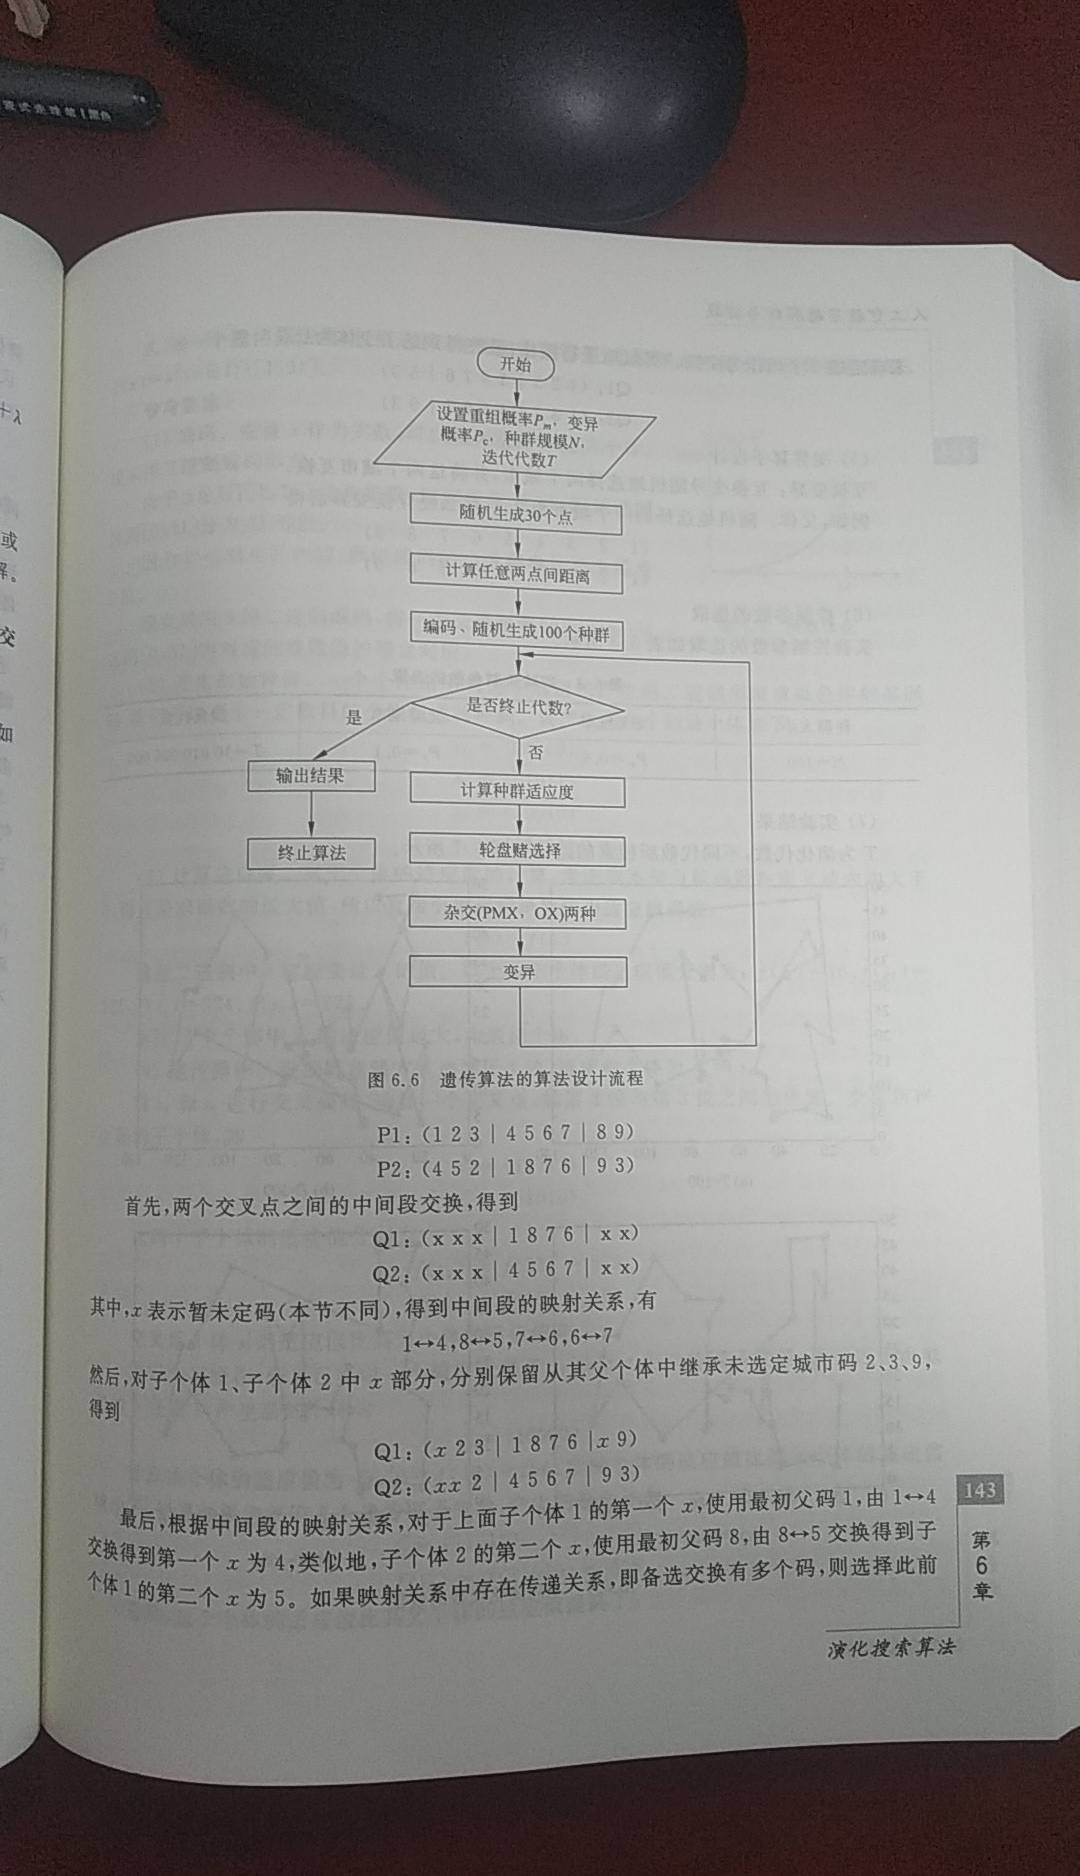
\includegraphics[width=0.8\textwidth]{28}
\end{figure}

Part B 任务三要求解析堆栈结构,检查堆栈返回地址是否合法。这里我们运行attack进行缓冲区溢出,实验结果如下。在这种检测方式下,我们认为只要eip不大于0xF0000就算合法,这是基于栈区往往在高地址而设置的。这种防御手段仅能防御住部分将代码放在栈区执行的缓冲区溢出攻击。对于我们在任务一实现的栈溢出攻击而言,第一种情况,也就是通过栈溢出跳转到代码段中的函数入口执行,这种防御手段无法防御,这种攻击手段常见于绕过保护验证;但对于第二种攻击手段,也就是构造shellcode放入栈区等到溢出后执行的攻击可以进行防御。

\begin{figure}[H]
	\centering
	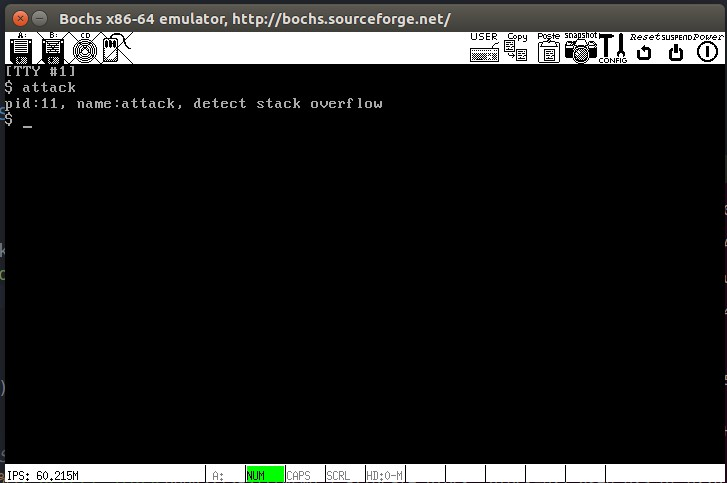
\includegraphics[width=0.8\textwidth]{whx18}
\end{figure}

\subsection{个人心得体会}
本次参与完成了所有实验,感觉越做越还挺有意思的。写多级反馈队列的刚开始本想造一个队列,然后用队列的操作去完成多级反馈调度,然后唐浩淼同学说既然是一个比较小型的多级反馈队列算法,就不用搞那么麻烦,提出要不直接在进程数据结构中加入字段也可以同样实现,随后我和王浩翔和唐浩淼三人完成了调度核心算法和打印性能评价。任务二加入自定义的功能,是我和庞紫萱同学在写密码学作业的时候,想起我们并没有调用太多c的库(除了printf),于是我们就想到把AES和DES算法移植到orangeos中。但其实移植过程也那么轻松,有许多需要转化的地方,比如数字转字符串、字符串转数字,orangeos的printf不支持十六进制输出我们又需要改动一些地方,工作量也不小。这一部分最后由我和庞紫萱和王浩翔三人共同完成。任务三shell多进程是我们在图书馆四人一起讨论出来的,这一部分我们改动的逻辑还是比较多的,我们考虑了如何全让父进程fork、如何fork结束后子进程能够进行多任务调度。写这一部分代码很容易一运行就不会再回显\$输入下一条指令,也就是很容易卡在某个地方,我们小组是花了一个上午四人一起不断调试最终成功的。任务四分页刚开始在图书馆讨论的时候放弃掉了,后来自己一个人回去想了下,感觉开启分页不难,就开始尝试了,不过就像实验报告所说,尝试到开启分页后,就不知道如何实现动态分配内存。偶然机会再上一届学长学姐的帮助下又进一步完成了一些,但是还没有完全完成。Part B部分都是我和王浩翔两人一起完成,其实我们选了linux的课程,对缓冲区溢出早早做过实验,所以任务一对于我们并不难写。任务二也是非常简单,我们很幸运在之前就移植了AES算法,所以我们在这里用了AES做了校验和,效果会比奇偶校验更好。任务三我们俩也对题目做了简化,我们刚开始看有点不太理解合法到底是什么意思,最后也是做了简化简单处理完成了任务三。


\newpage

\section{指导教师评语及成绩}
\noindent
【评语】
\begin{table}[H]
\centering
%\renewcommand\tablename{表}		  		% 将’Table 1'更改为'表 1'
%\setlength{\abovecaptionskip}{0pt}	 	% 自己设置caption的上间距
%\setlength{\belowcaptionskip}{5pt}		% 自己设置caption的下间距
\setlength{\tabcolsep}{7mm}			% 可以调表的总宽度
\scalebox{1}{							% 可以调整表格整体大小
\begin{tabular}{cccccccccc}
 &  &  &  &  &  &       &  &         &  \\
     &  &  &  &  &  &       &  &         &  \\
     &  &  &  &  &  &       &  &         &  \\
     &  &  &  &  &  &       &  &         &  \\
     &  &  &  &  &  &       &  &         &  \\
     &  &  &  &  &  &       &  &         &  \\
     &  &  &  &  &  &       &  &         &  \\
     &  &  &  &  &  &       &  &         &  \\
     &  &  &  &  &  & 成\quad\quad 绩:   &  & 指导老师签名: &  \\
     &  &  &  &  &  & 批阅日期: &  &         & 
\end{tabular}
}
\end{table}
\end{document}